% Created 2021-02-13 sáb 09:34
% Intended LaTeX compiler: pdflatex
\documentclass{SelfArx}
  \usepackage[T1]{fontenc}
\usepackage[utf8]{inputenc}
\usepackage{booktabs}
\renewcommand{\arraystretch}{1.1} % Unclear
\usepackage{graphicx}
\usepackage{float}
\usepackage{amsmath}
\usepackage{csquotes}
\setlength{\fboxrule}{0.75pt} % Width of the border around the abstract
\definecolor{color1}{RGB}{0,0,90} % Color of the article title and sections
\definecolor{color2}{RGB}{0,20,20} % Color of the boxes behind the abstract and headings
\usepackage[portuguese, english]{babel} % Specify a different language here - english by default
\usepackage{lipsum} % Required to insert dummy text. To be removed otherwise
\usepackage[backend=biber,%
style = abnt,%
noslsn, %
isbn = false,
url = false,
extrayear, %
uniquename=init,%
giveninits, %
justify, %
sccite,%
scbib, %
sorting=nyt,
% mergedate=compact,
% natbib=true,
repeattitles, %
maxcitenames=3]{biblatex}
\AtEveryBibitem{%
\clearfield{urlyear}
\clearfield{urlmonth}
\clearfield{note}
\clearfield{issn} % Remove issn
\clearfield{doi} % Remove doi
\ifentrytype{online}{}{% Remove url except for @online
\clearfield{url}
}
}
\date{}
\title{Dados: O PIB da pandemia e cenários para 2021}
\begin{document}

\JournalInfo{Nota de Conjuntura No 15} % Journal information
\Archive{} % Additional notes (e.g. copyright, DOI, review/research article)

\Authors{Pedro Paulo Zahluth Bastos\textsuperscript{1}*, Lorena Dourado\textsuperscript{2}, Gabriel Petrini\textsuperscript{3}, Antônio Ibarra\textsuperscript{3}}} % Authors
\affiliation{\textsuperscript{1}\textit{Professor do Instituto de Economia Unicamp}} % Author affiliation
\affiliation{\textsuperscript{2}\textit{Graduanda do Instituto de Economia Unicamp}} % Author affiliation
\affiliation{\textsuperscript{3}\textit{Doutorando do Instituto de Economia  Unicamp}} % Author affiliation
\affiliation{*\textbf{E-mail}: ppzbastos@gmail.com} % Corresponding author

\Keywords{Keyword1 --- Keyword2 --- Keyword3} % Keywords - if you don't want any simply remove all the text between the curly brackets
\newcommand{\keywordname}{Palavras-chave} % Defines the keywords heading name

\Abstract{
\begin{itemize}

\item Em março, havia risco de sucessão longa de quedas trimestrais do PIB, com círculo vicioso de contração de demanda, contração do crédito, falências de empresas e ampliação do desemprego e da pobreza.
\item O risco foi contornado com política anticíclica para sustentar renda, vínculos empregatícios e, tardiamente, ampliação do crédito (apesar do repasse da depreciação cambial).
\item A continuidade da pandemia limitou a retomada da demanda e do emprego em serviços em razão do risco de contágio, reafirmando a centralidade do controle da pandemia para a recuperação da economia (não há trade-off duradouro).
\item A magnitude da política anticíclica gera um risco enorme de um segundo mergulho em razão da retomada da lei do teto do gasto e da retirada brusca dos programas emergenciais.
\item Sem política anticíclica, aumento do desemprego e da pobreza serão dramáticos ainda que as exportações se recuperem em 2021.
\end{itemize}
}
\renewcommand{\abstractname}{Sumário Executivo} % Defines the keywords heading name
\flushbottom % Makes all text pages the same height
\maketitle % Print the title and abstract box
\thispagestyle{empty} % Removes page numbering from the first page
\onecolumn

\section*{Indicadores de antecedente}
\label{sec:org80faa25}
\subsection*{IBC-Br (acumulado 12 meses vs 12 meses anteriores)}
\label{sec:orgd9f3203}

\begin{center}
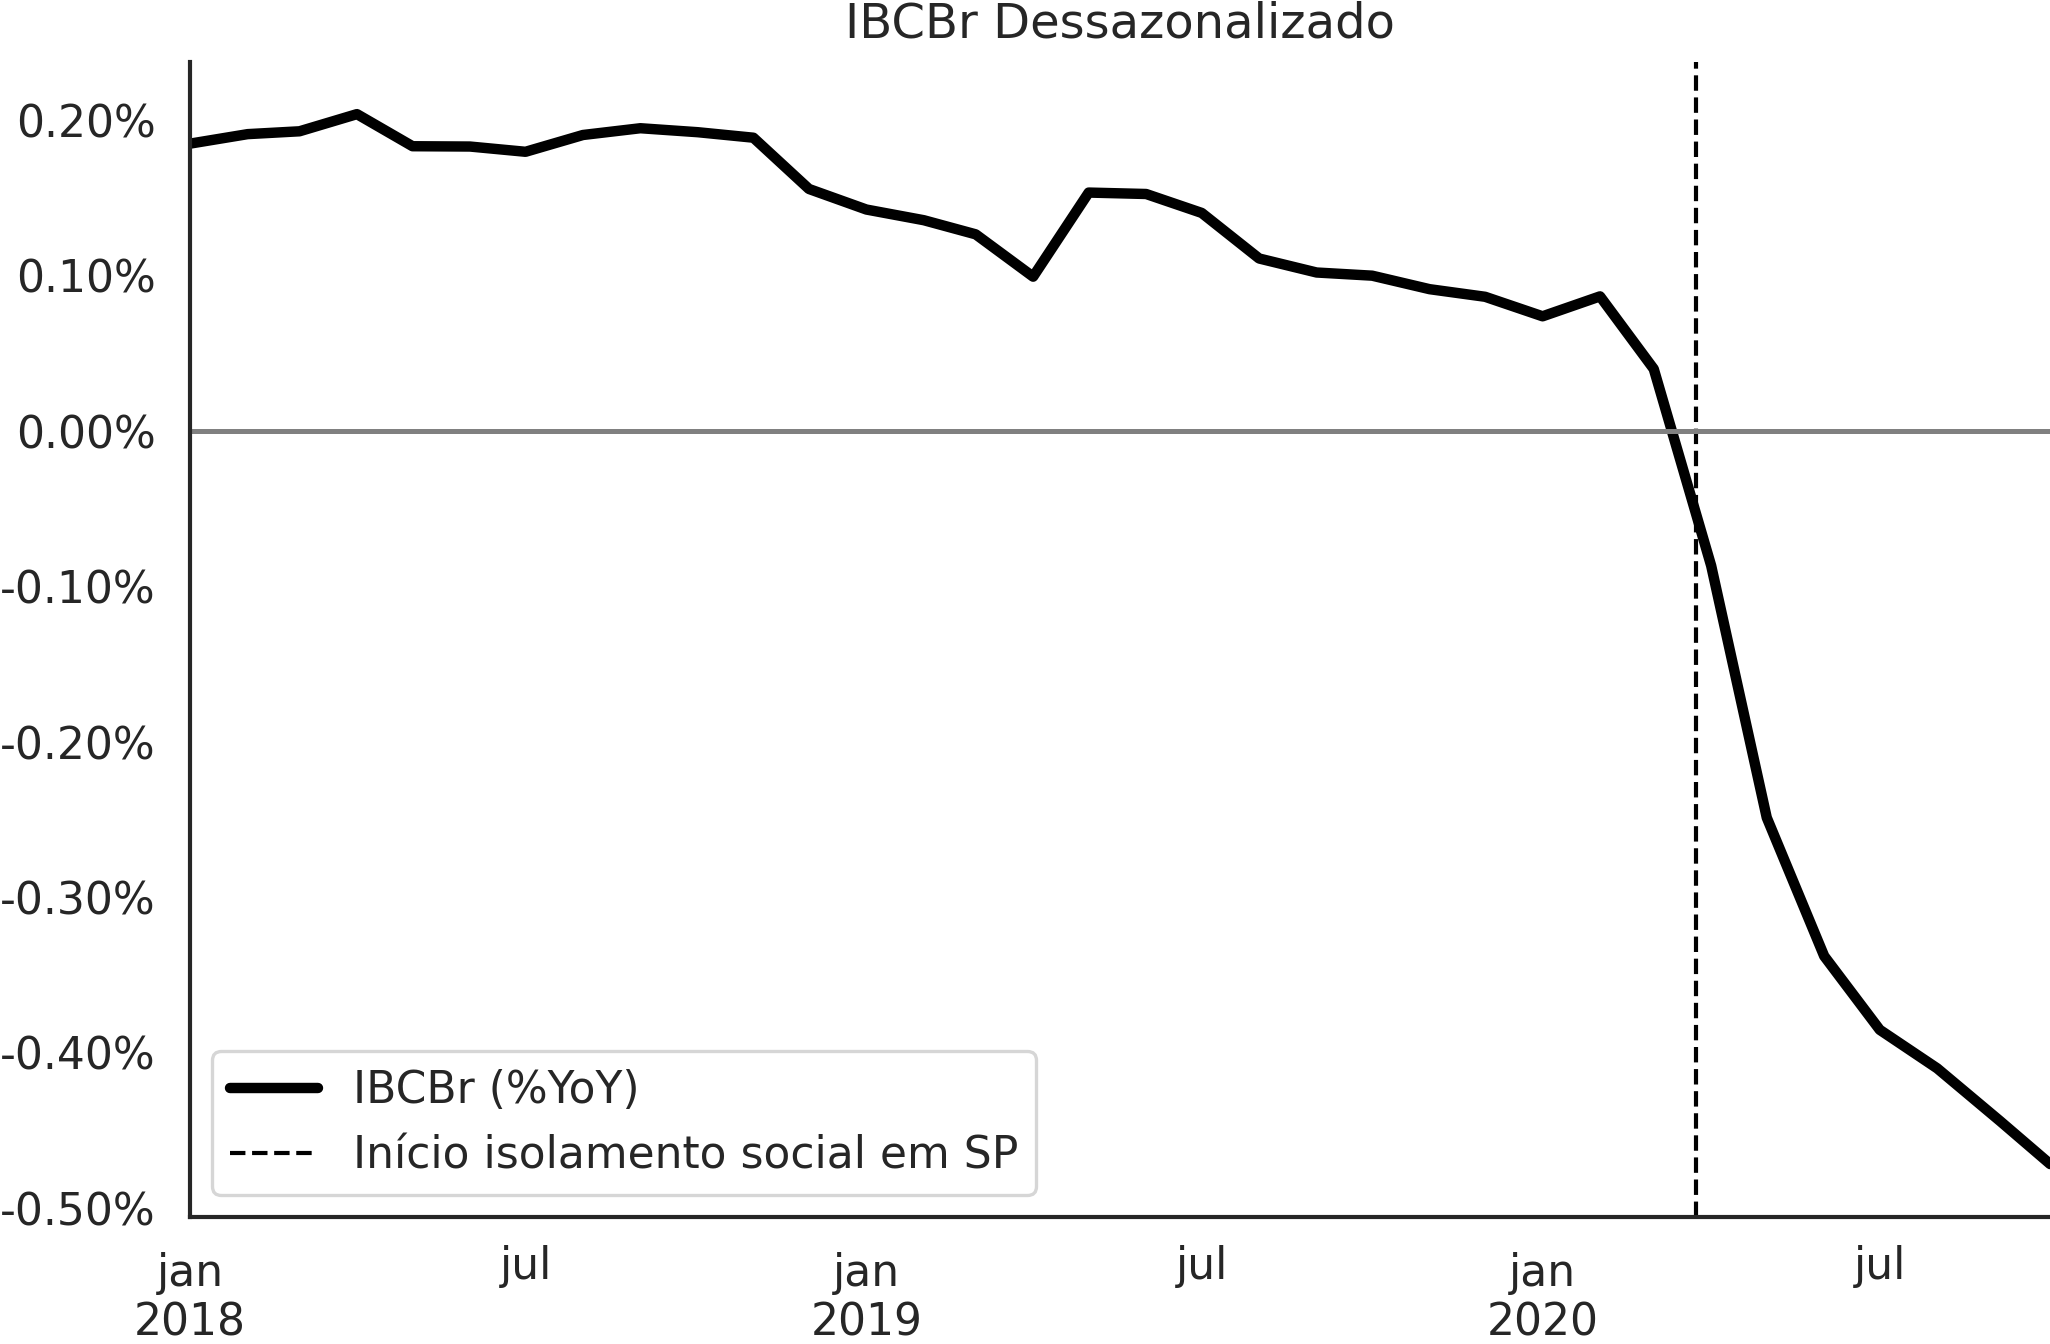
\includegraphics[width=.9\linewidth]{./figs/Antecedente/IBCBr.png}
\end{center}

\subsection*{Tráfego de veículos pesados nas estradas pedagiadas - ABCR - Dados dessazonalizados}
\label{sec:orgae43ea9}


\begin{center}
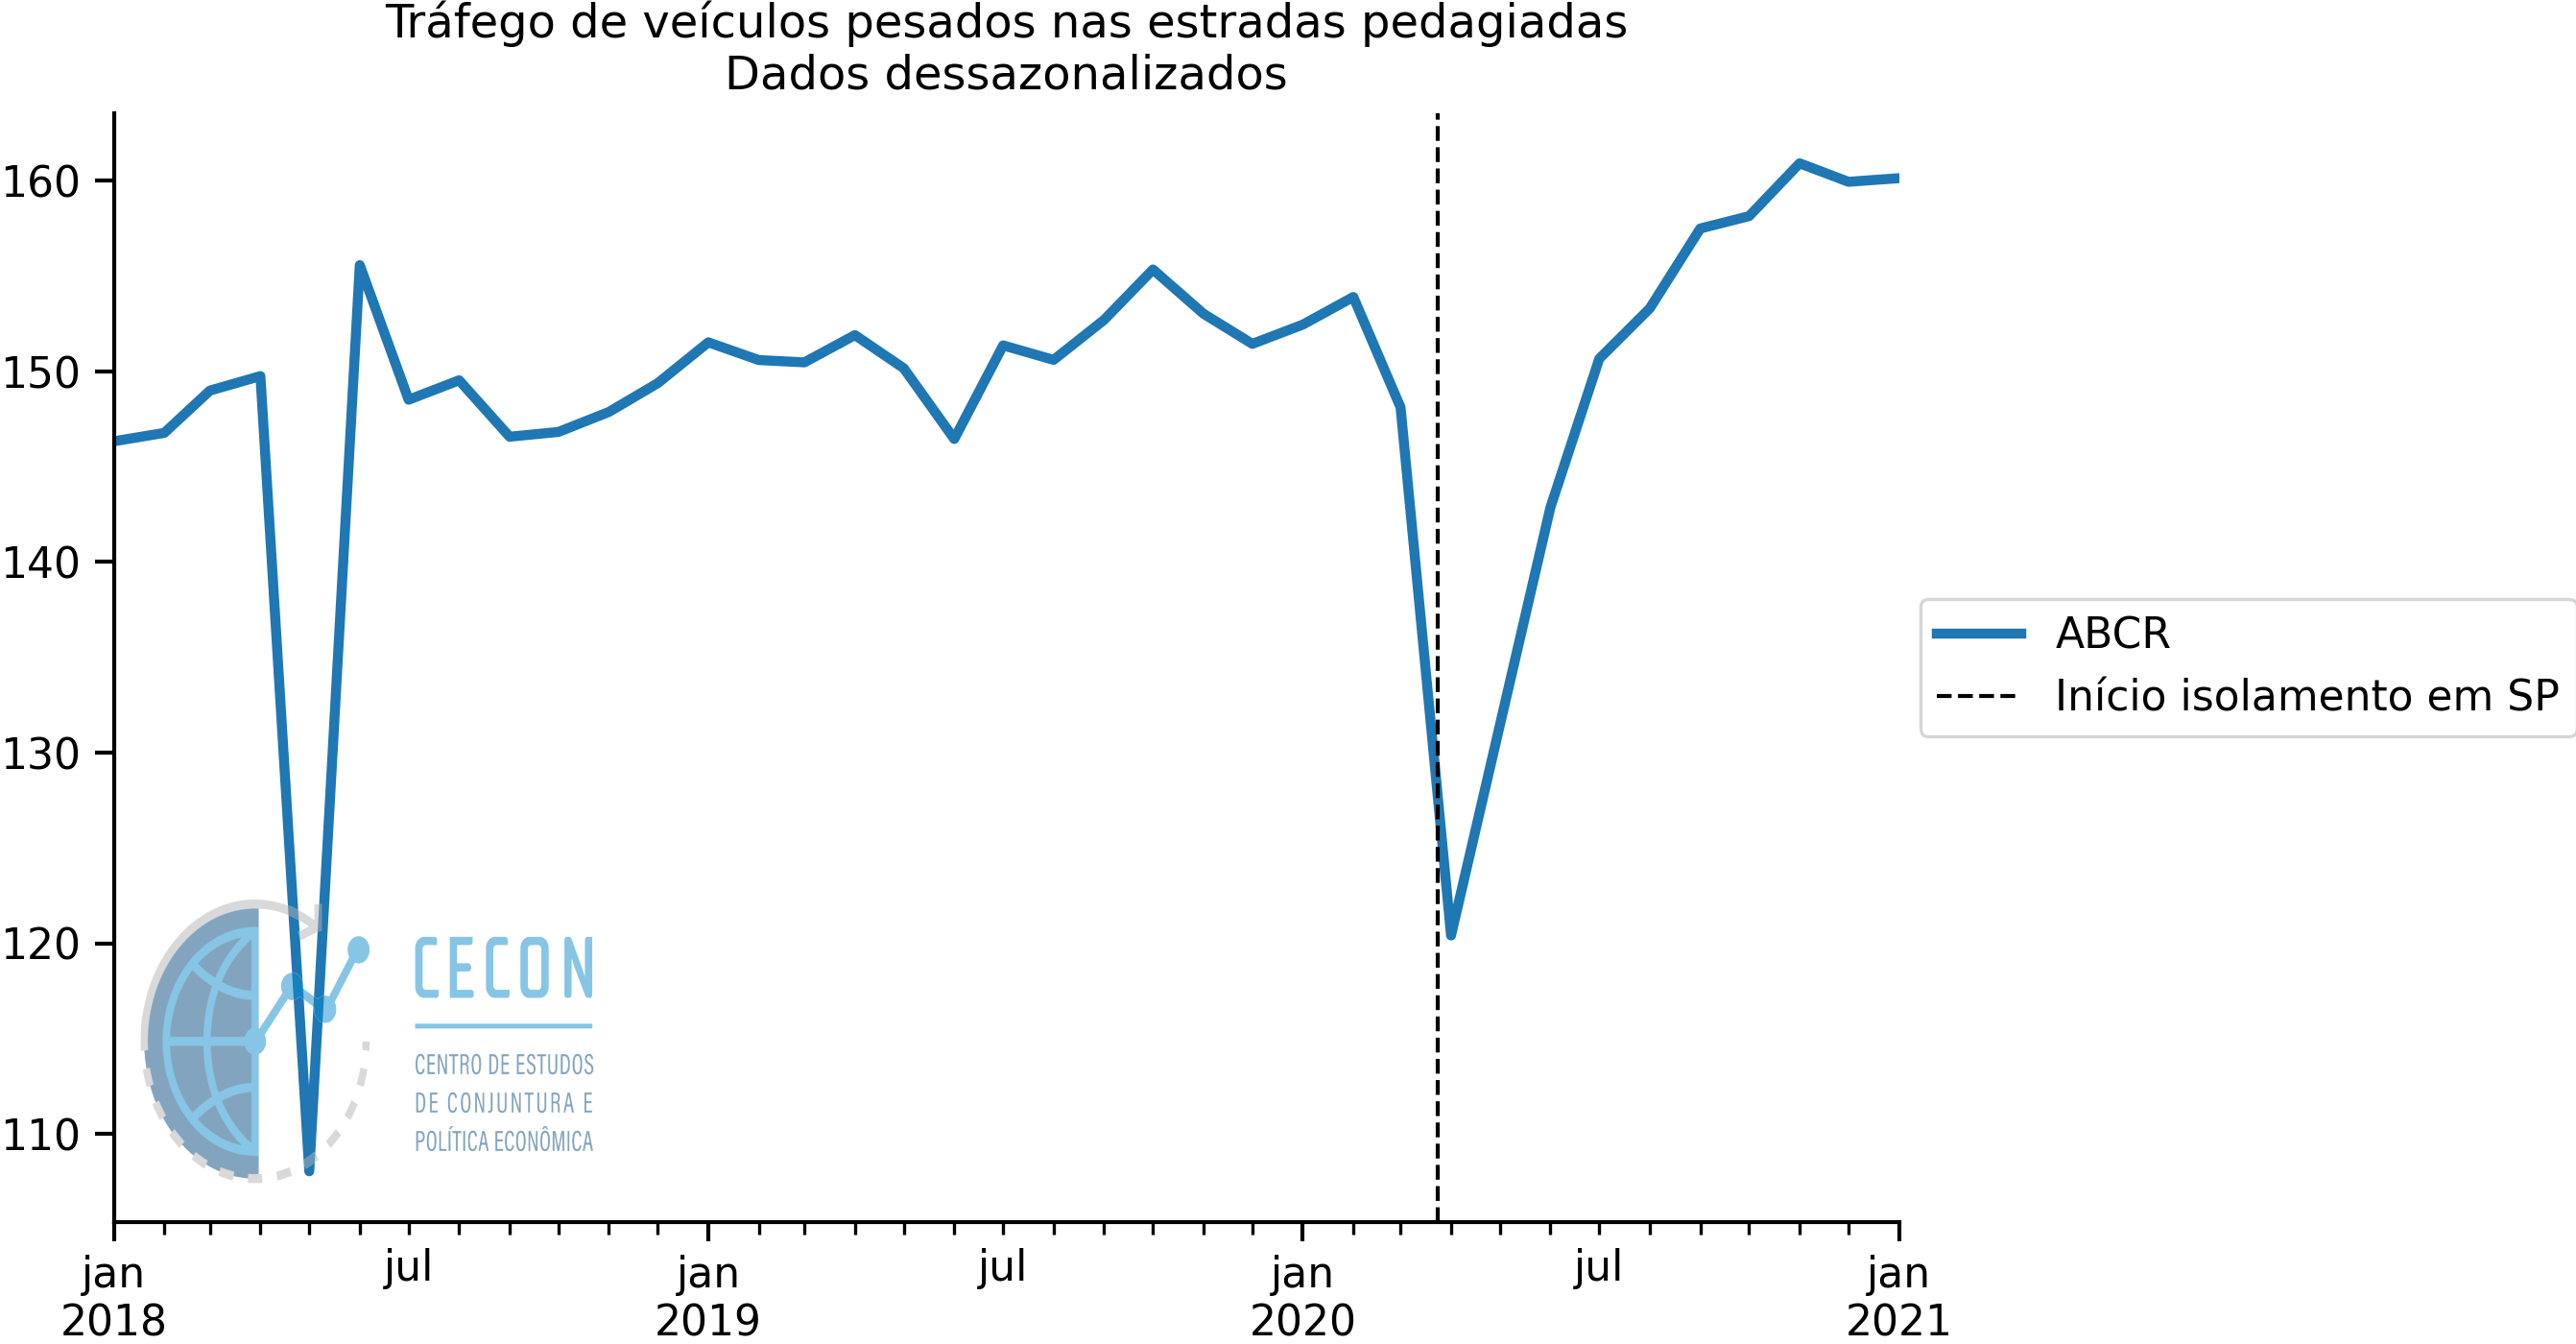
\includegraphics[width=.9\linewidth]{./figs/Setoriais/TrafegoPedagio.png}
\end{center}


\section*{Dados de alta frequência}
\label{sec:orgc7756df}

\subsection*{Bloomberg adaptado ao COVID-19 (\href{https://www.bloomberg.com/news/articles/2020-11-13/alternative-data-show-activity-crashes-as-virus-resurges-chart}{Link})}
\label{sec:org5cde0d4}

\subsection*{Google Reports: Brasil}
\label{sec:org07a2e13}

\begin{center}
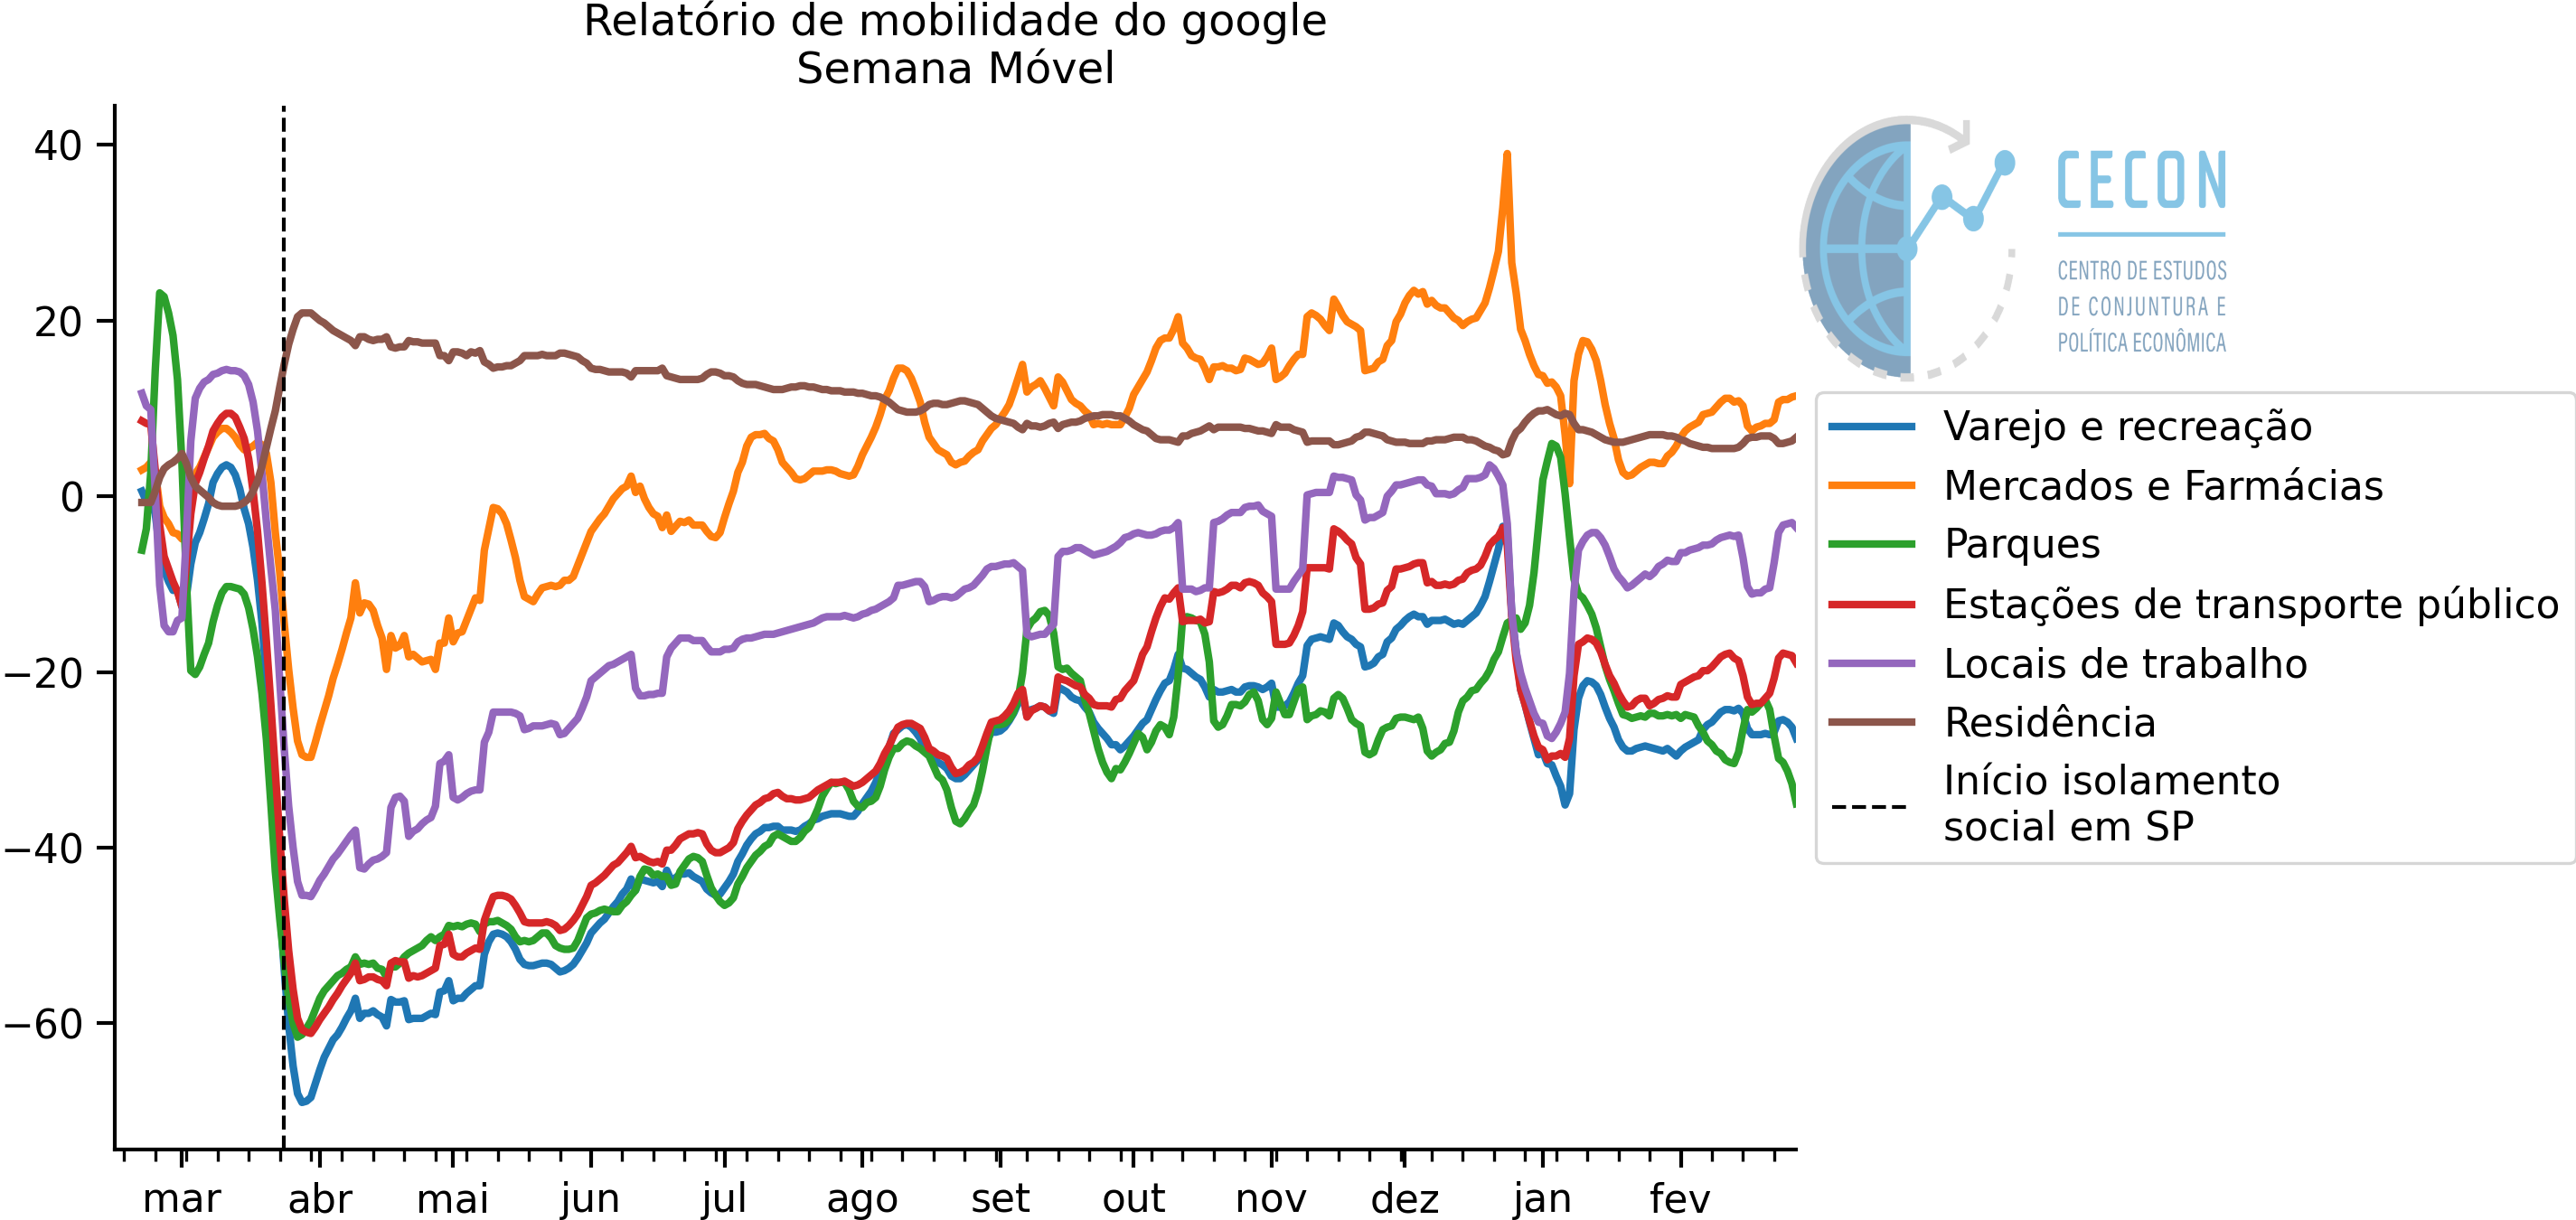
\includegraphics[width=.9\linewidth]{./figs/Granulares/GoogleReport_Brasil.png}
\end{center}

\subsection*{Apple: Tendências de mobilidade}
\label{sec:orgf92855c}

\begin{center}
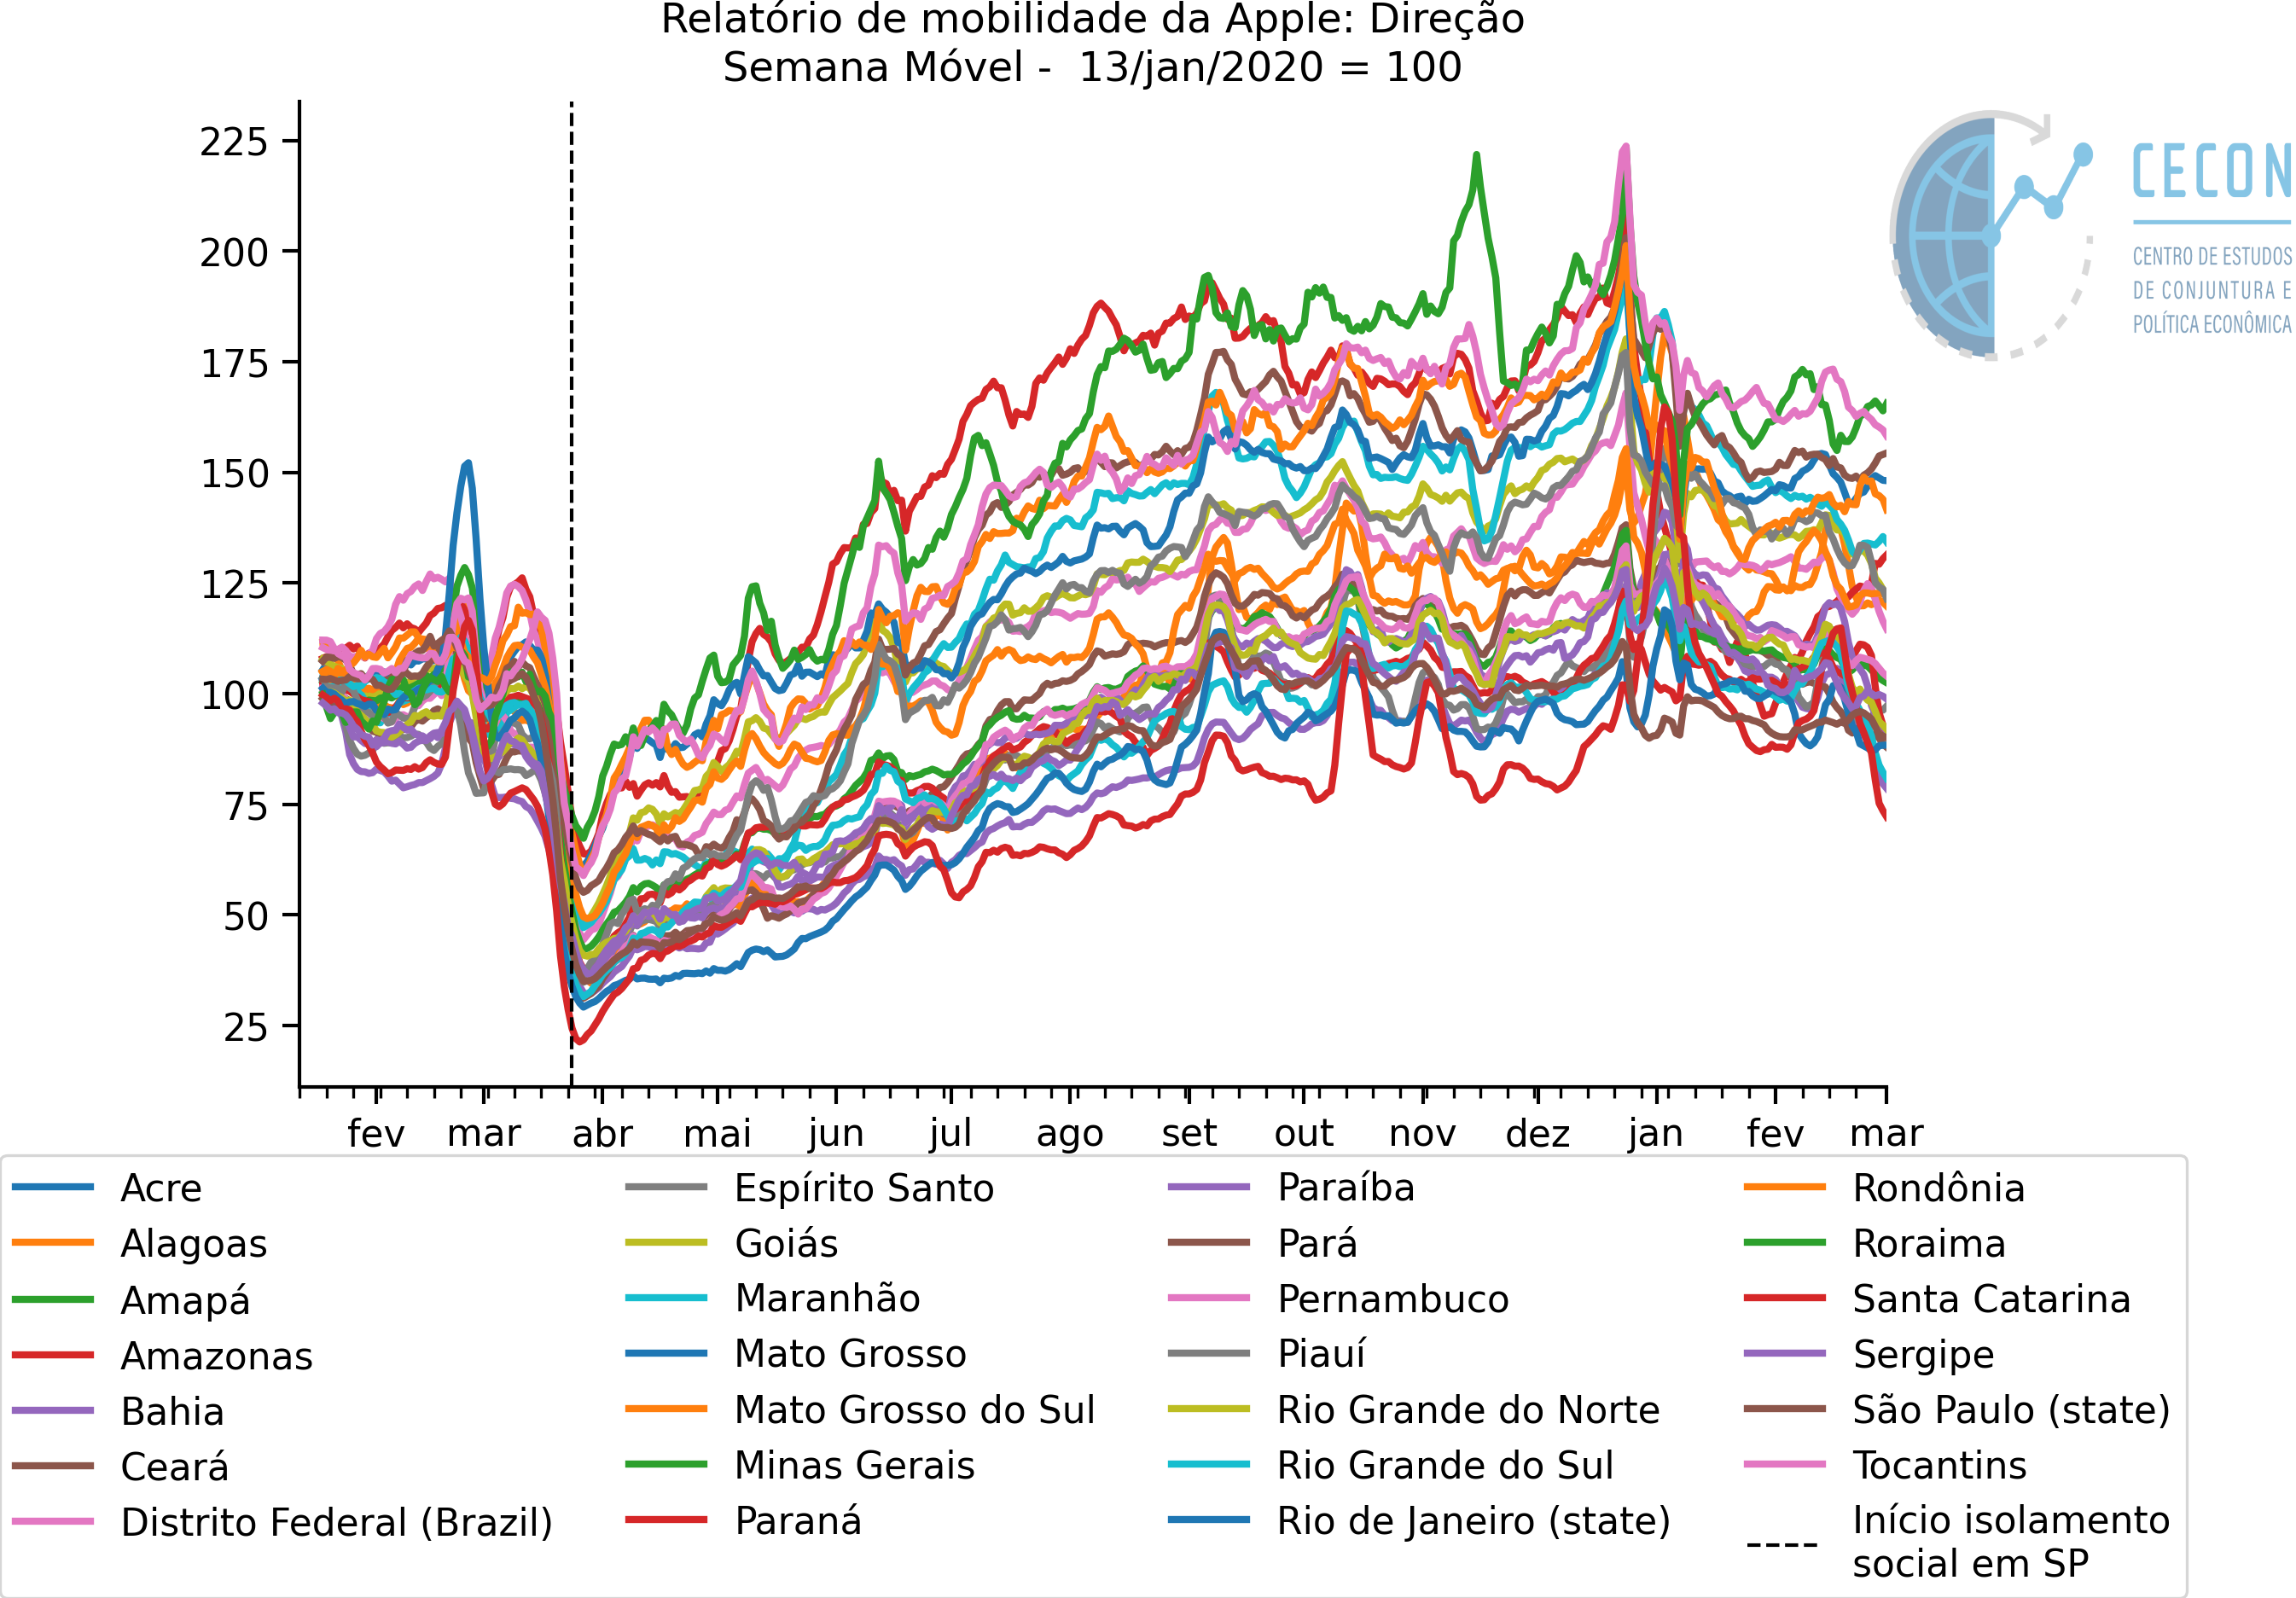
\includegraphics[width=.9\linewidth]{./figs/Granulares/AppleReport_Brasil.png}
\end{center}

\subsection*{Waze: \(\Delta \%\) Km}
\label{sec:org0cdf910}

\begin{center}
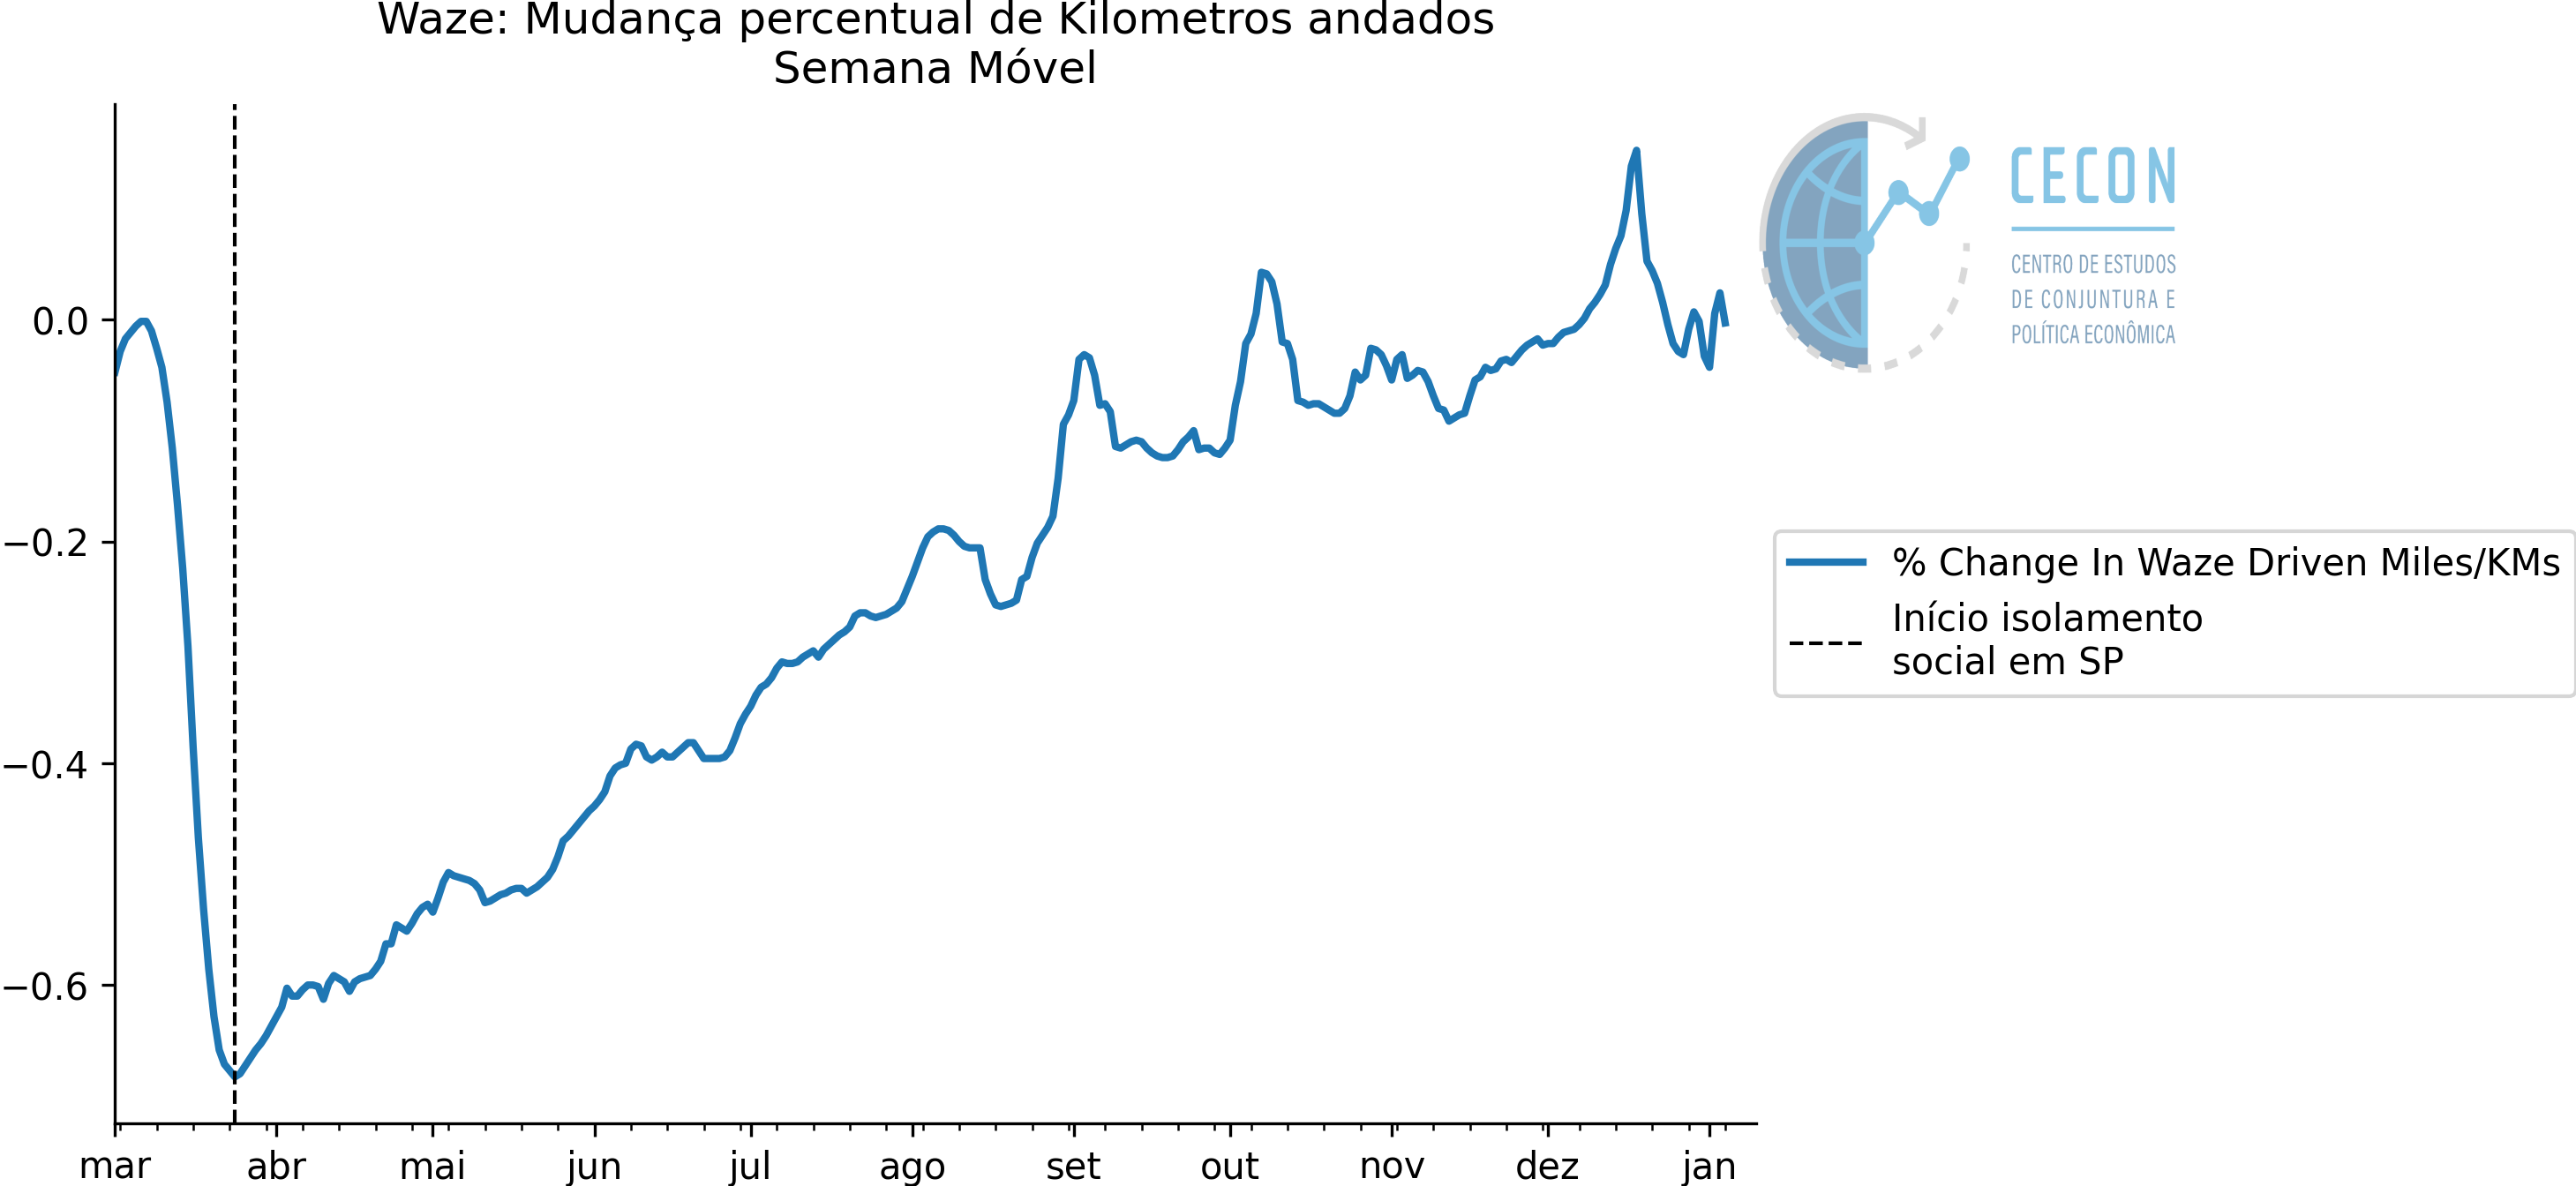
\includegraphics[width=.9\linewidth]{./figs/Granulares/Waze_Brasil.png}
\end{center}

\subsection*{TomTom: Congestionamento}
\label{sec:org630a31b}

\begin{center}
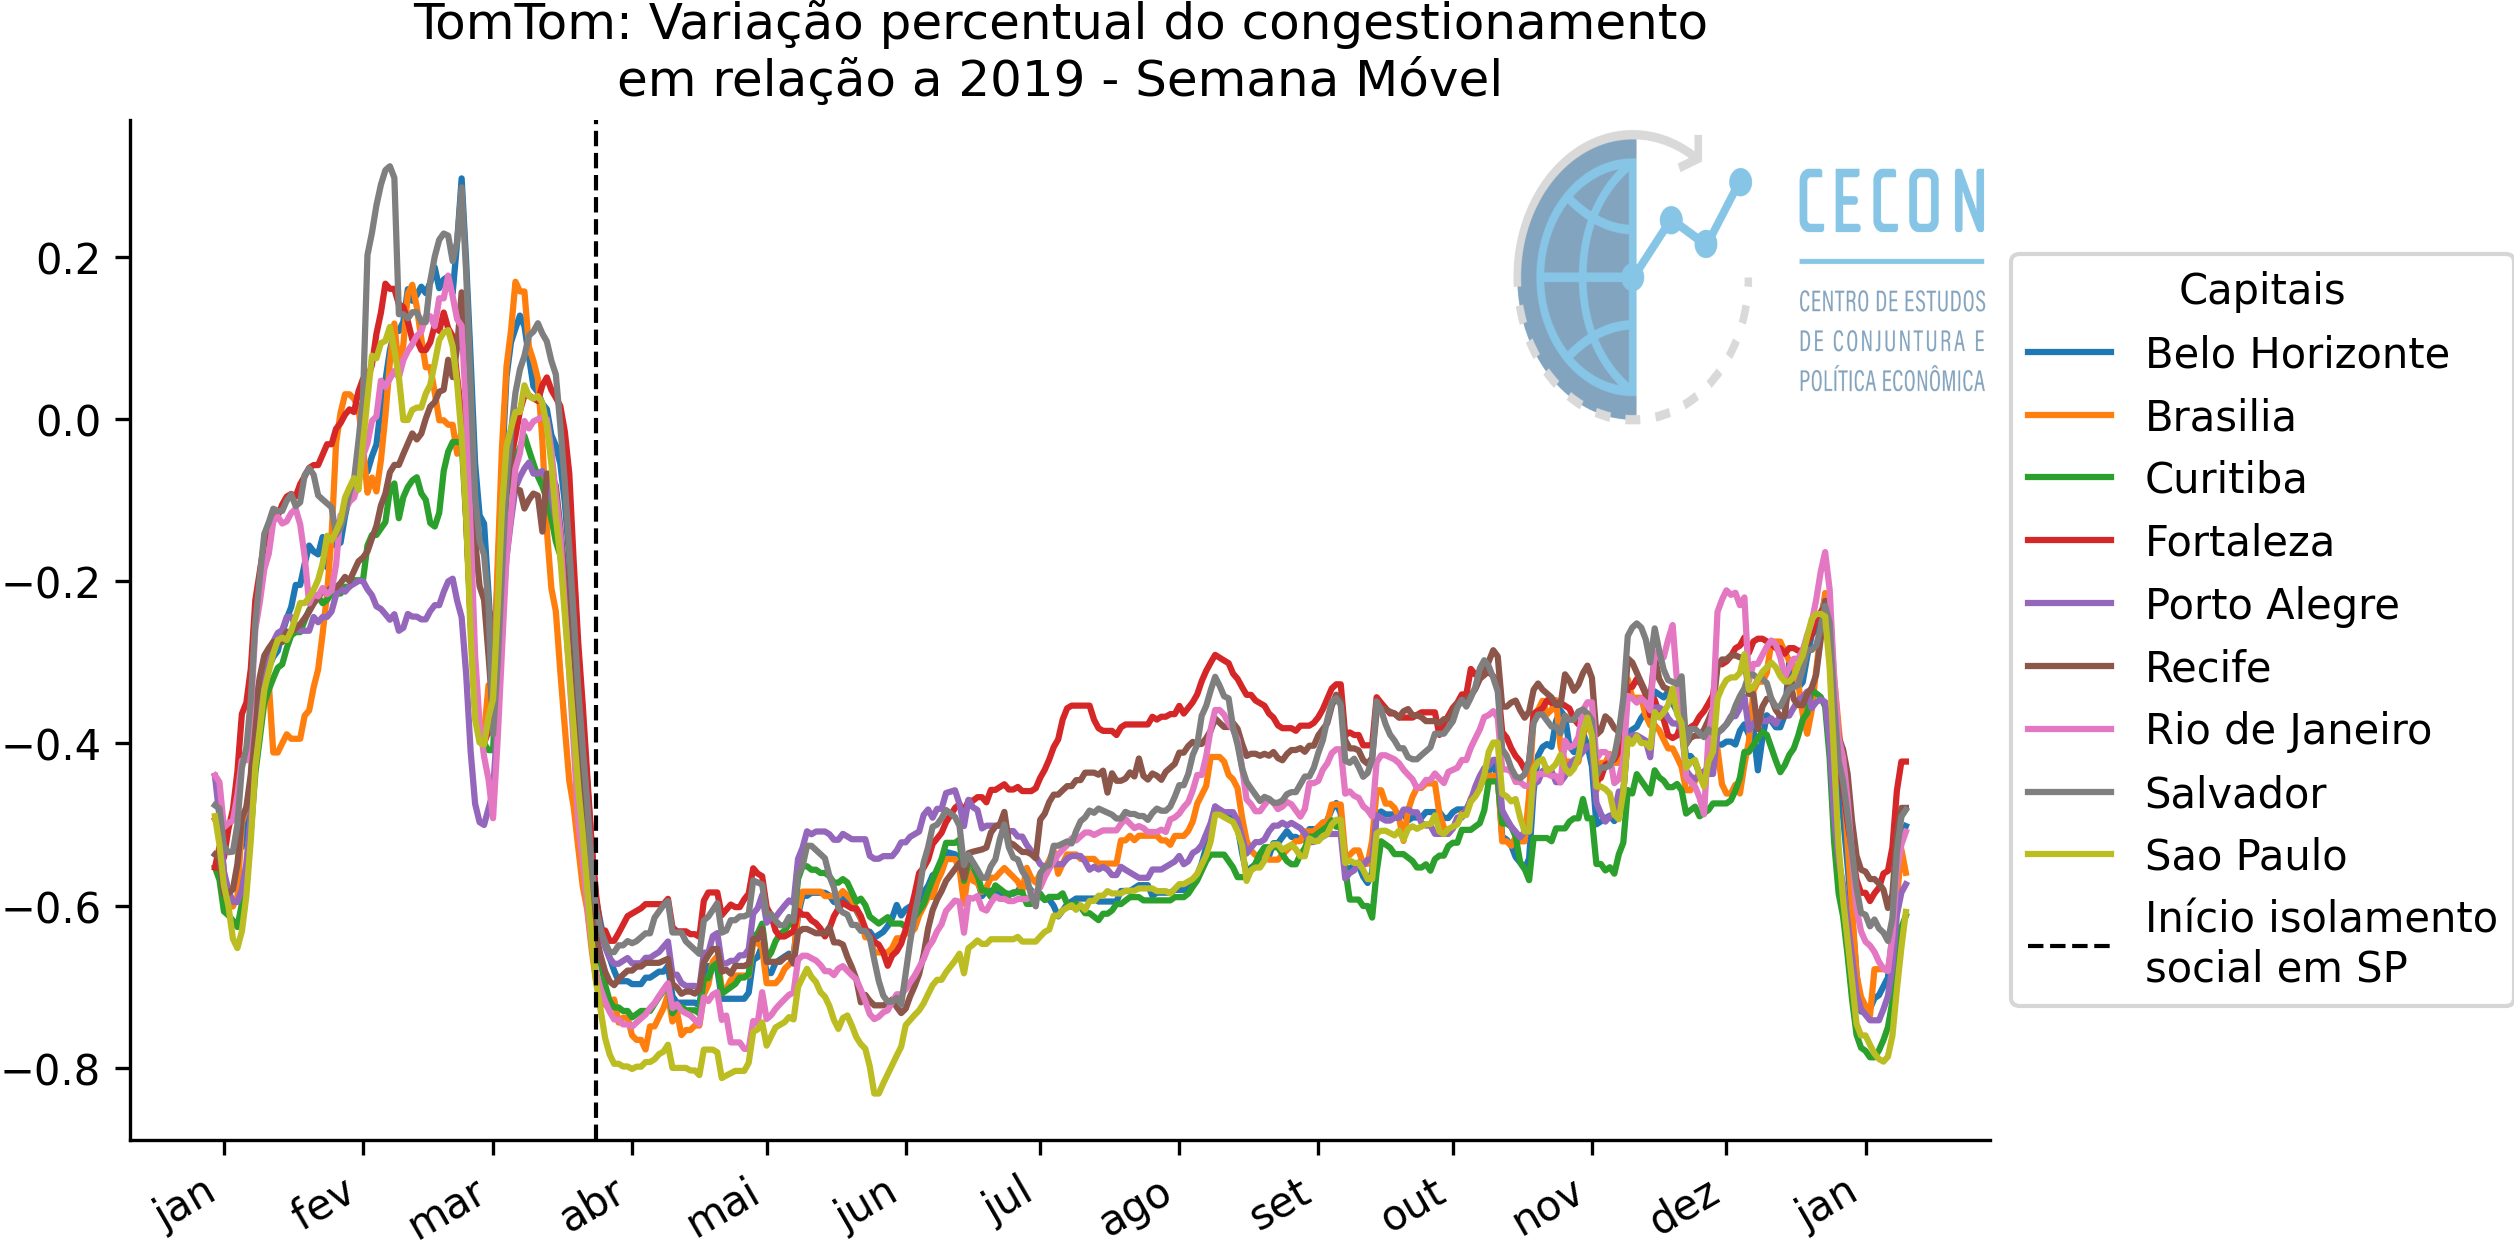
\includegraphics[width=.9\linewidth]{./figs/Granulares/TomTom_Brasil.png}
\end{center}

\section*{Atividade}
\label{sec:org371ceee}



\subsection*{Trimestre Contra trimestre imediatamente anterior}
\label{sec:orgc7d434c}

\begin{center}
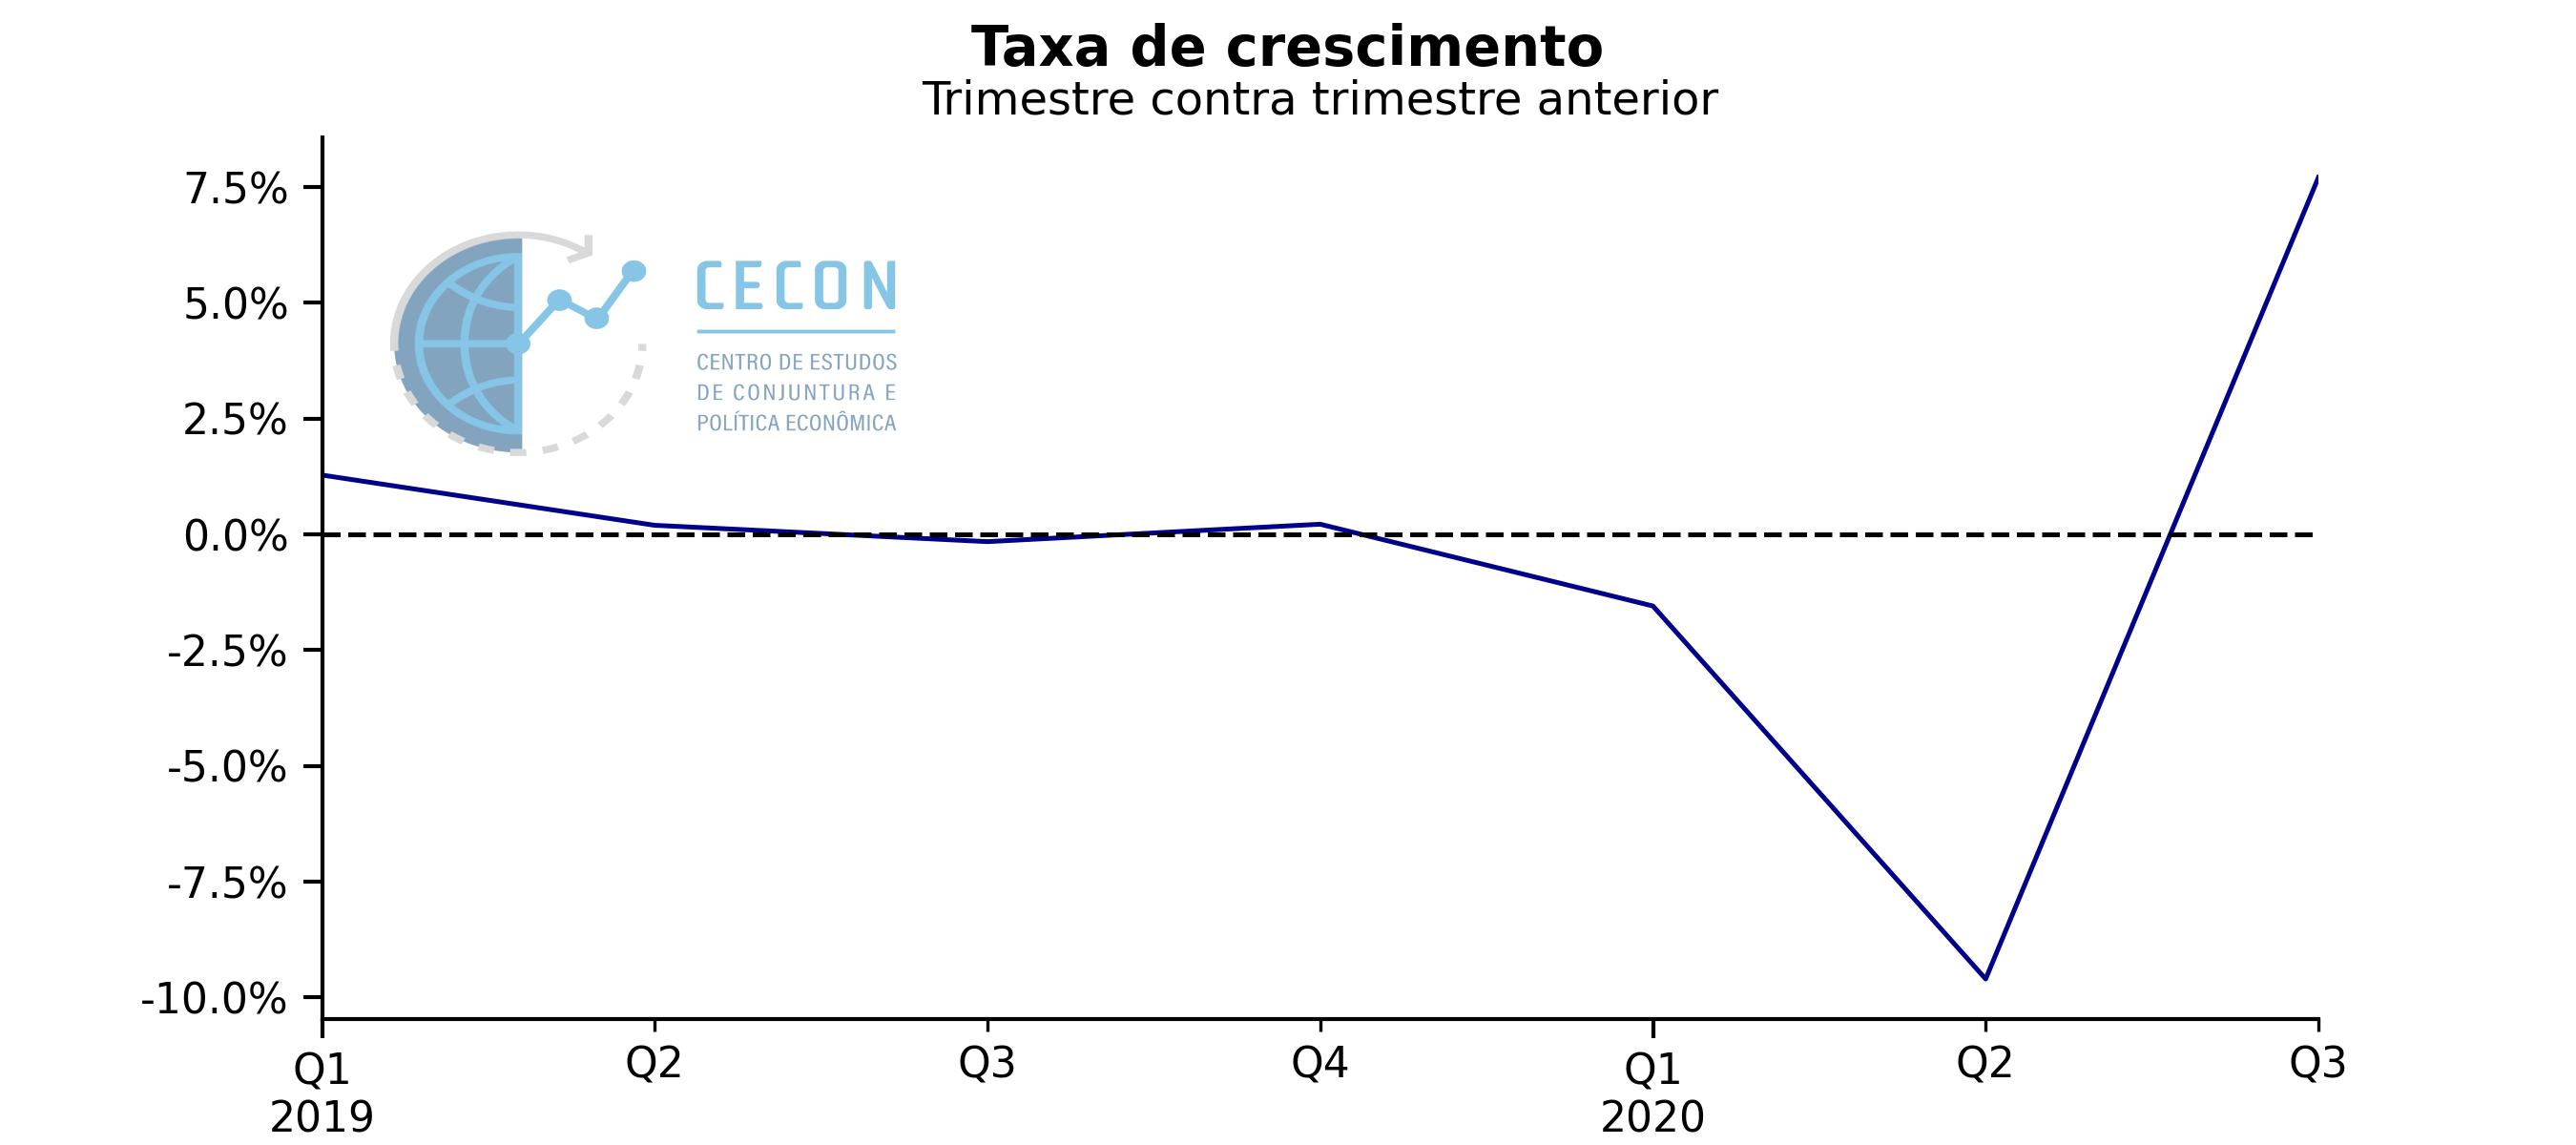
\includegraphics[width=.9\linewidth]{./figs/PIB/PIB.png}
\end{center}

\subsection*{Trimestre Contra mesmo trimestre do ano anterior}
\label{sec:org404e110}

\begin{center}
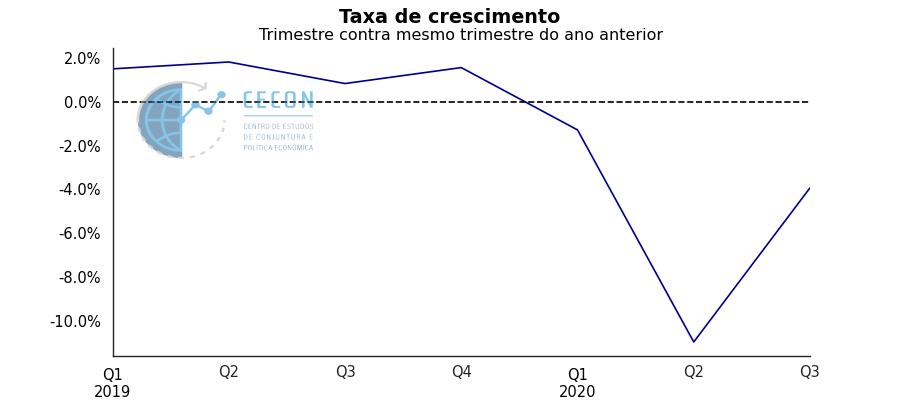
\includegraphics[width=.9\linewidth]{./figs/PIB/PIB_YoY.png}
\end{center}

\subsection*{Agropecuária}
\label{sec:orgb4486bb}

\begin{center}
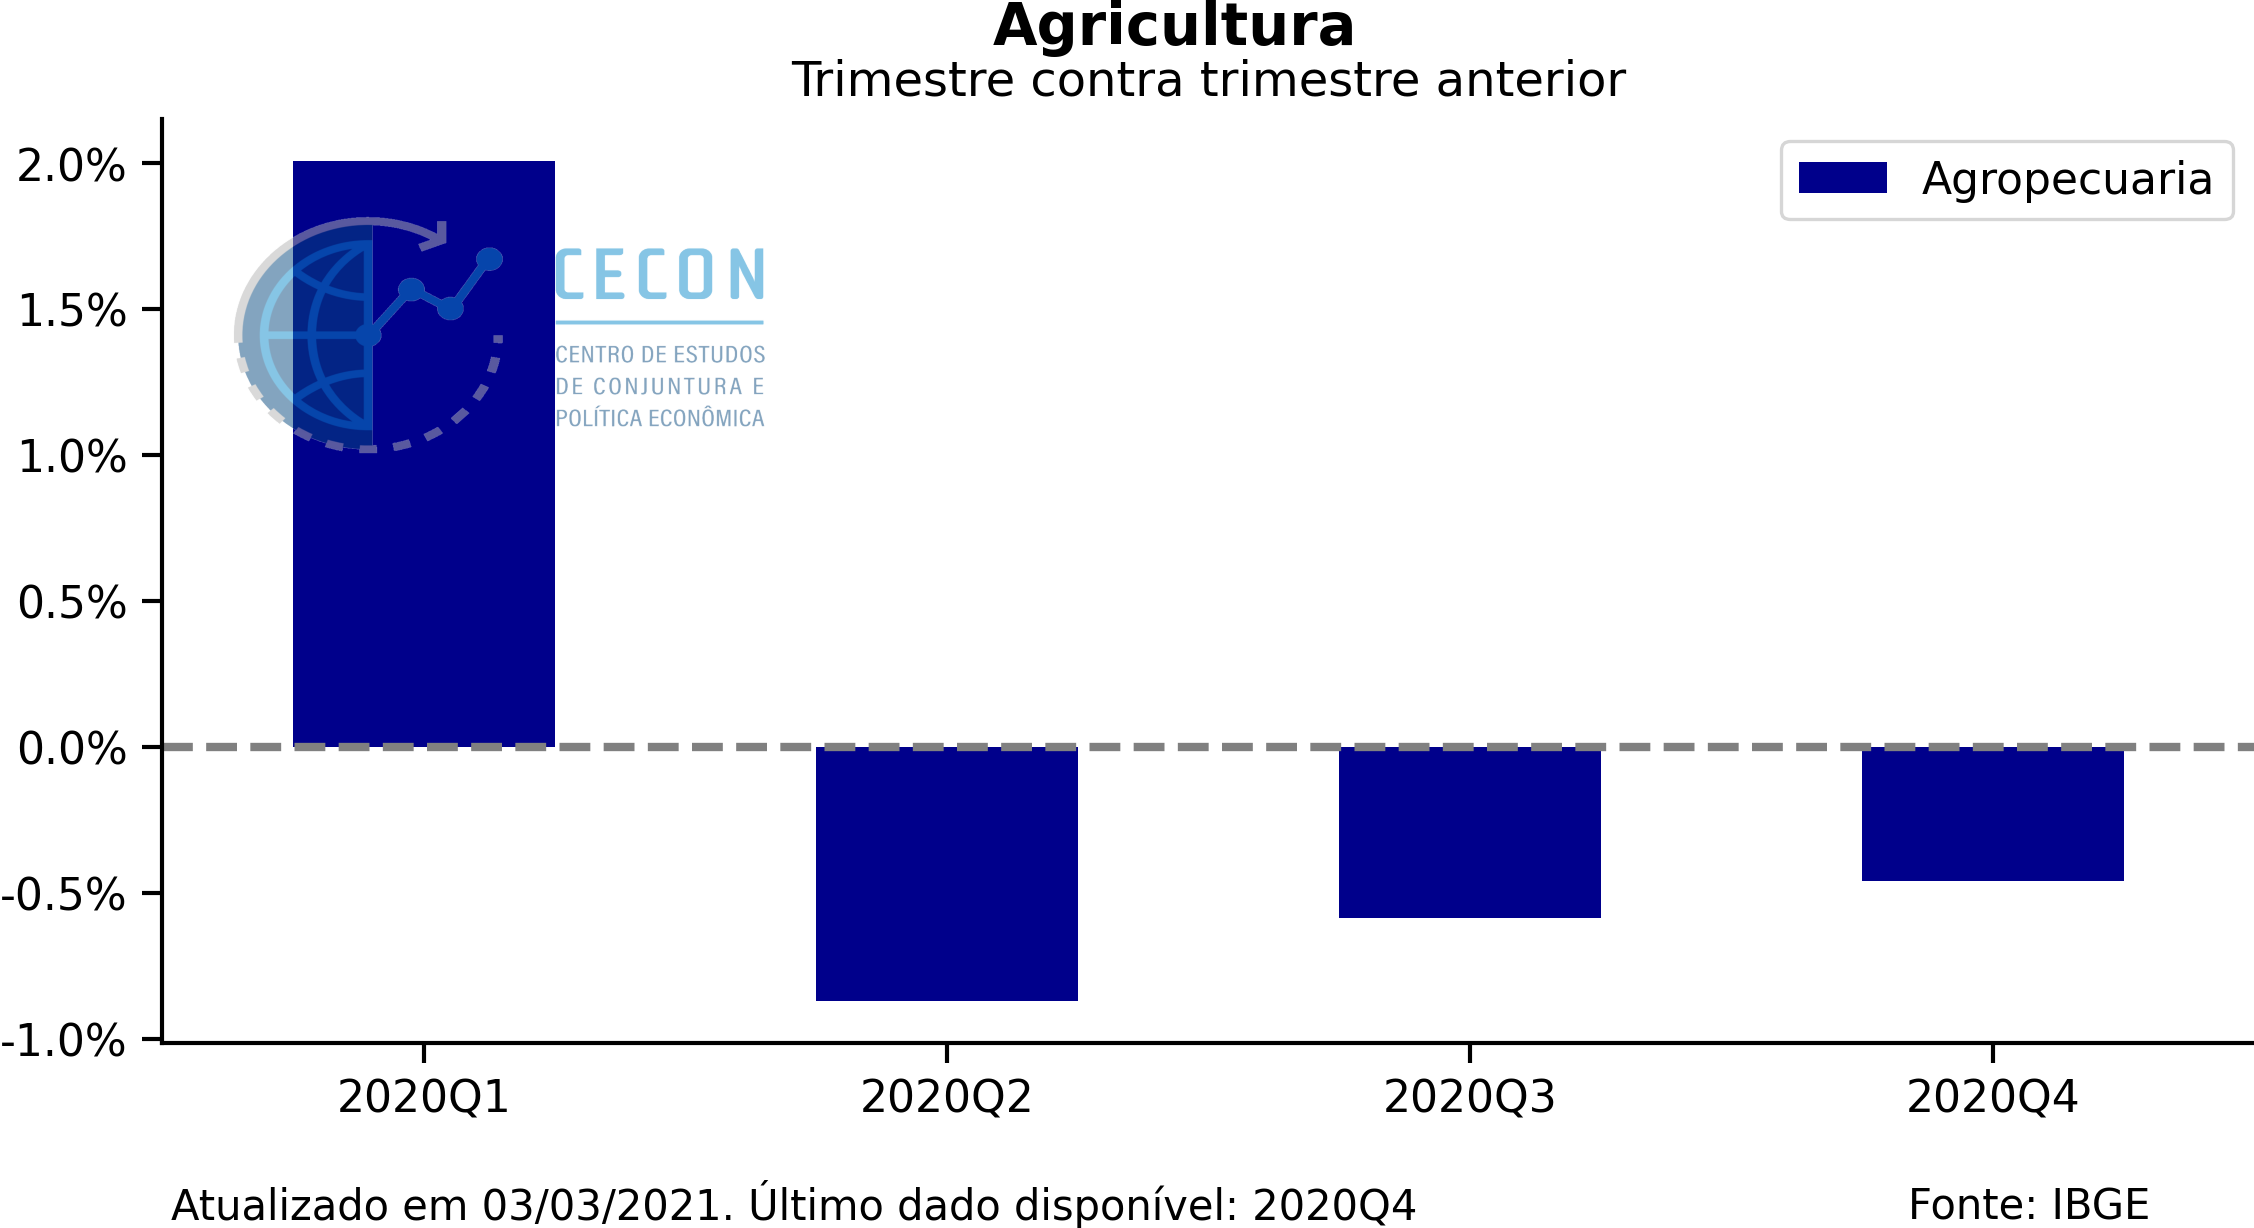
\includegraphics[width=.9\linewidth]{./figs/PIB/Agropecuaria.png}
\end{center}

\subsection*{Indústria}
\label{sec:org532be0a}

\begin{center}
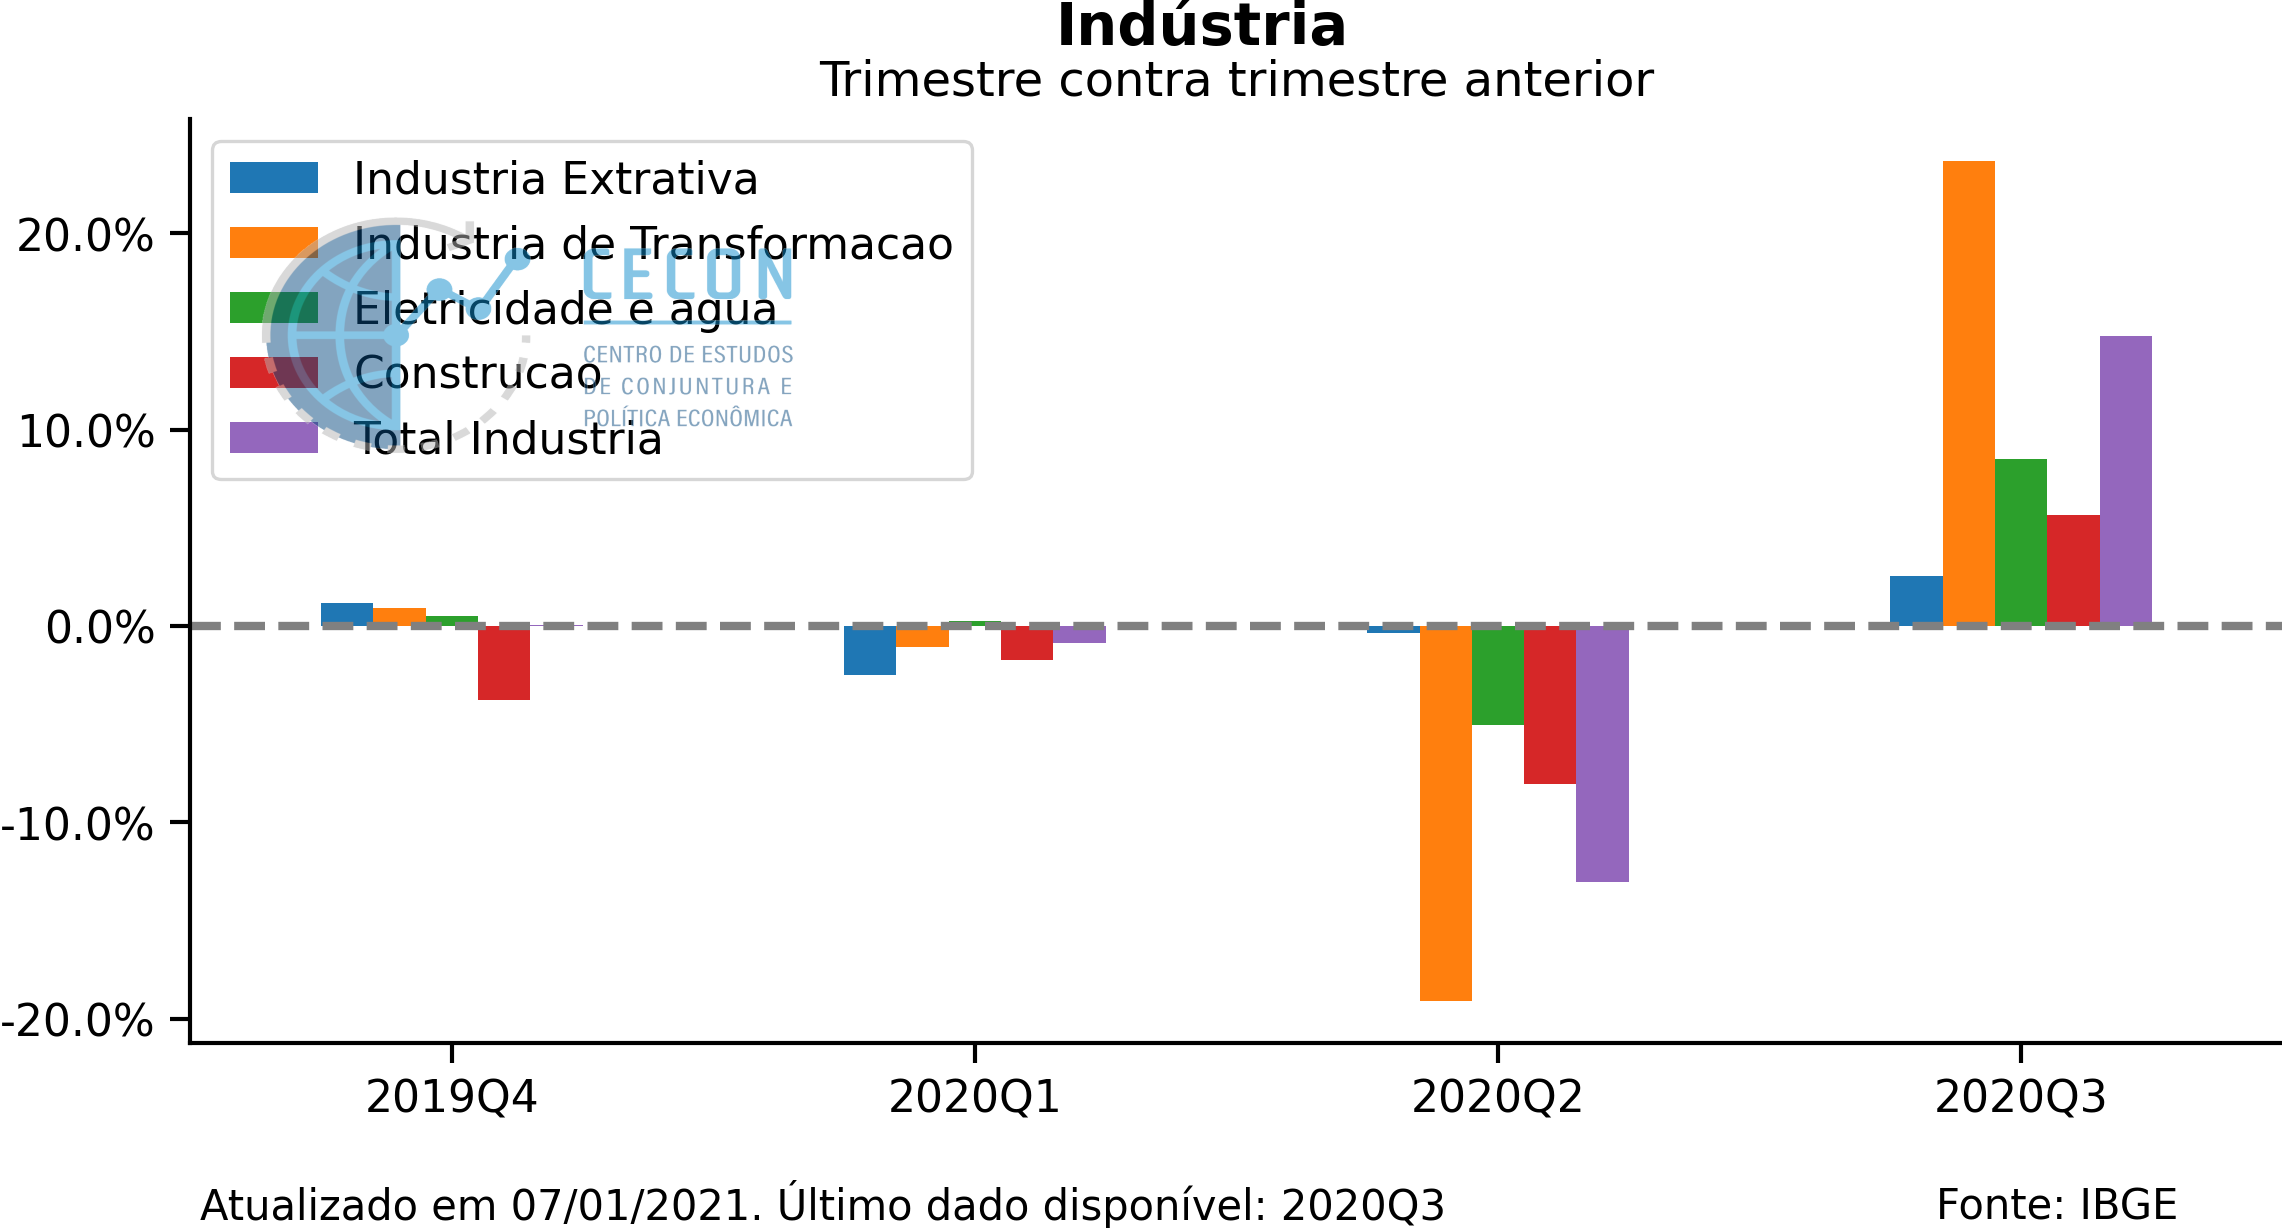
\includegraphics[width=.9\linewidth]{./figs/PIB/Industria.png}
\end{center}


\subsection*{Serviços}
\label{sec:org44d0b5e}

\begin{center}
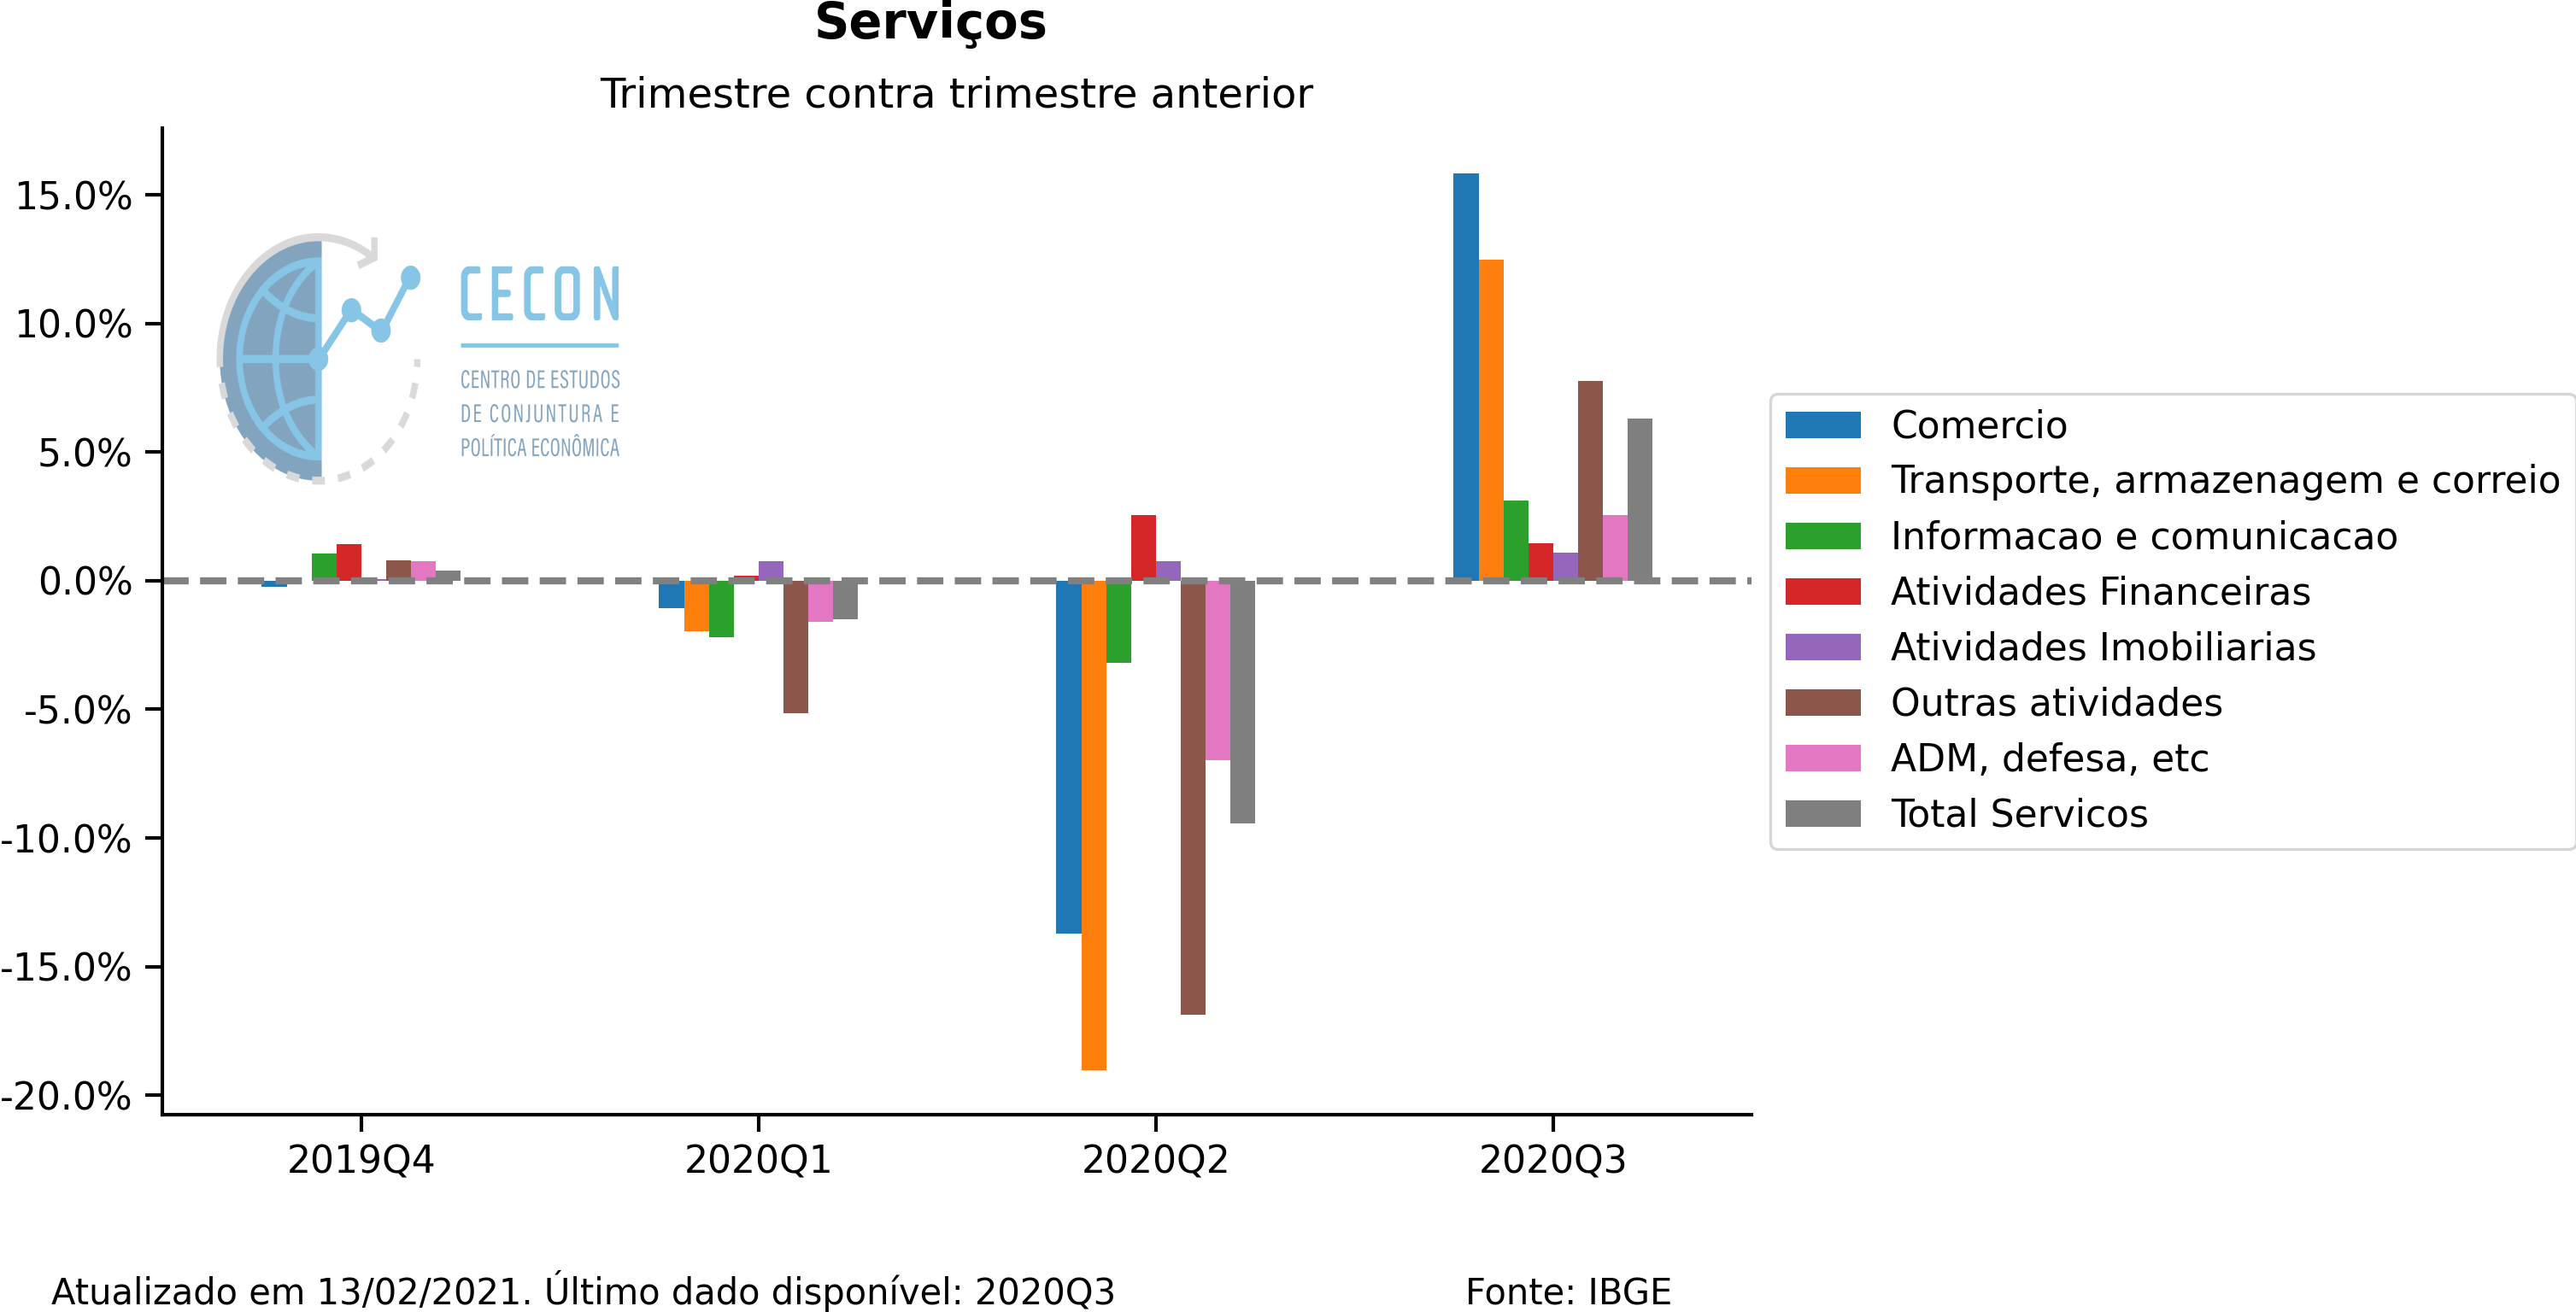
\includegraphics[width=.9\linewidth]{./figs/PIB/Servicos.png}
\end{center}

\subsection*{Demanda}
\label{sec:org284b61e}

\begin{center}
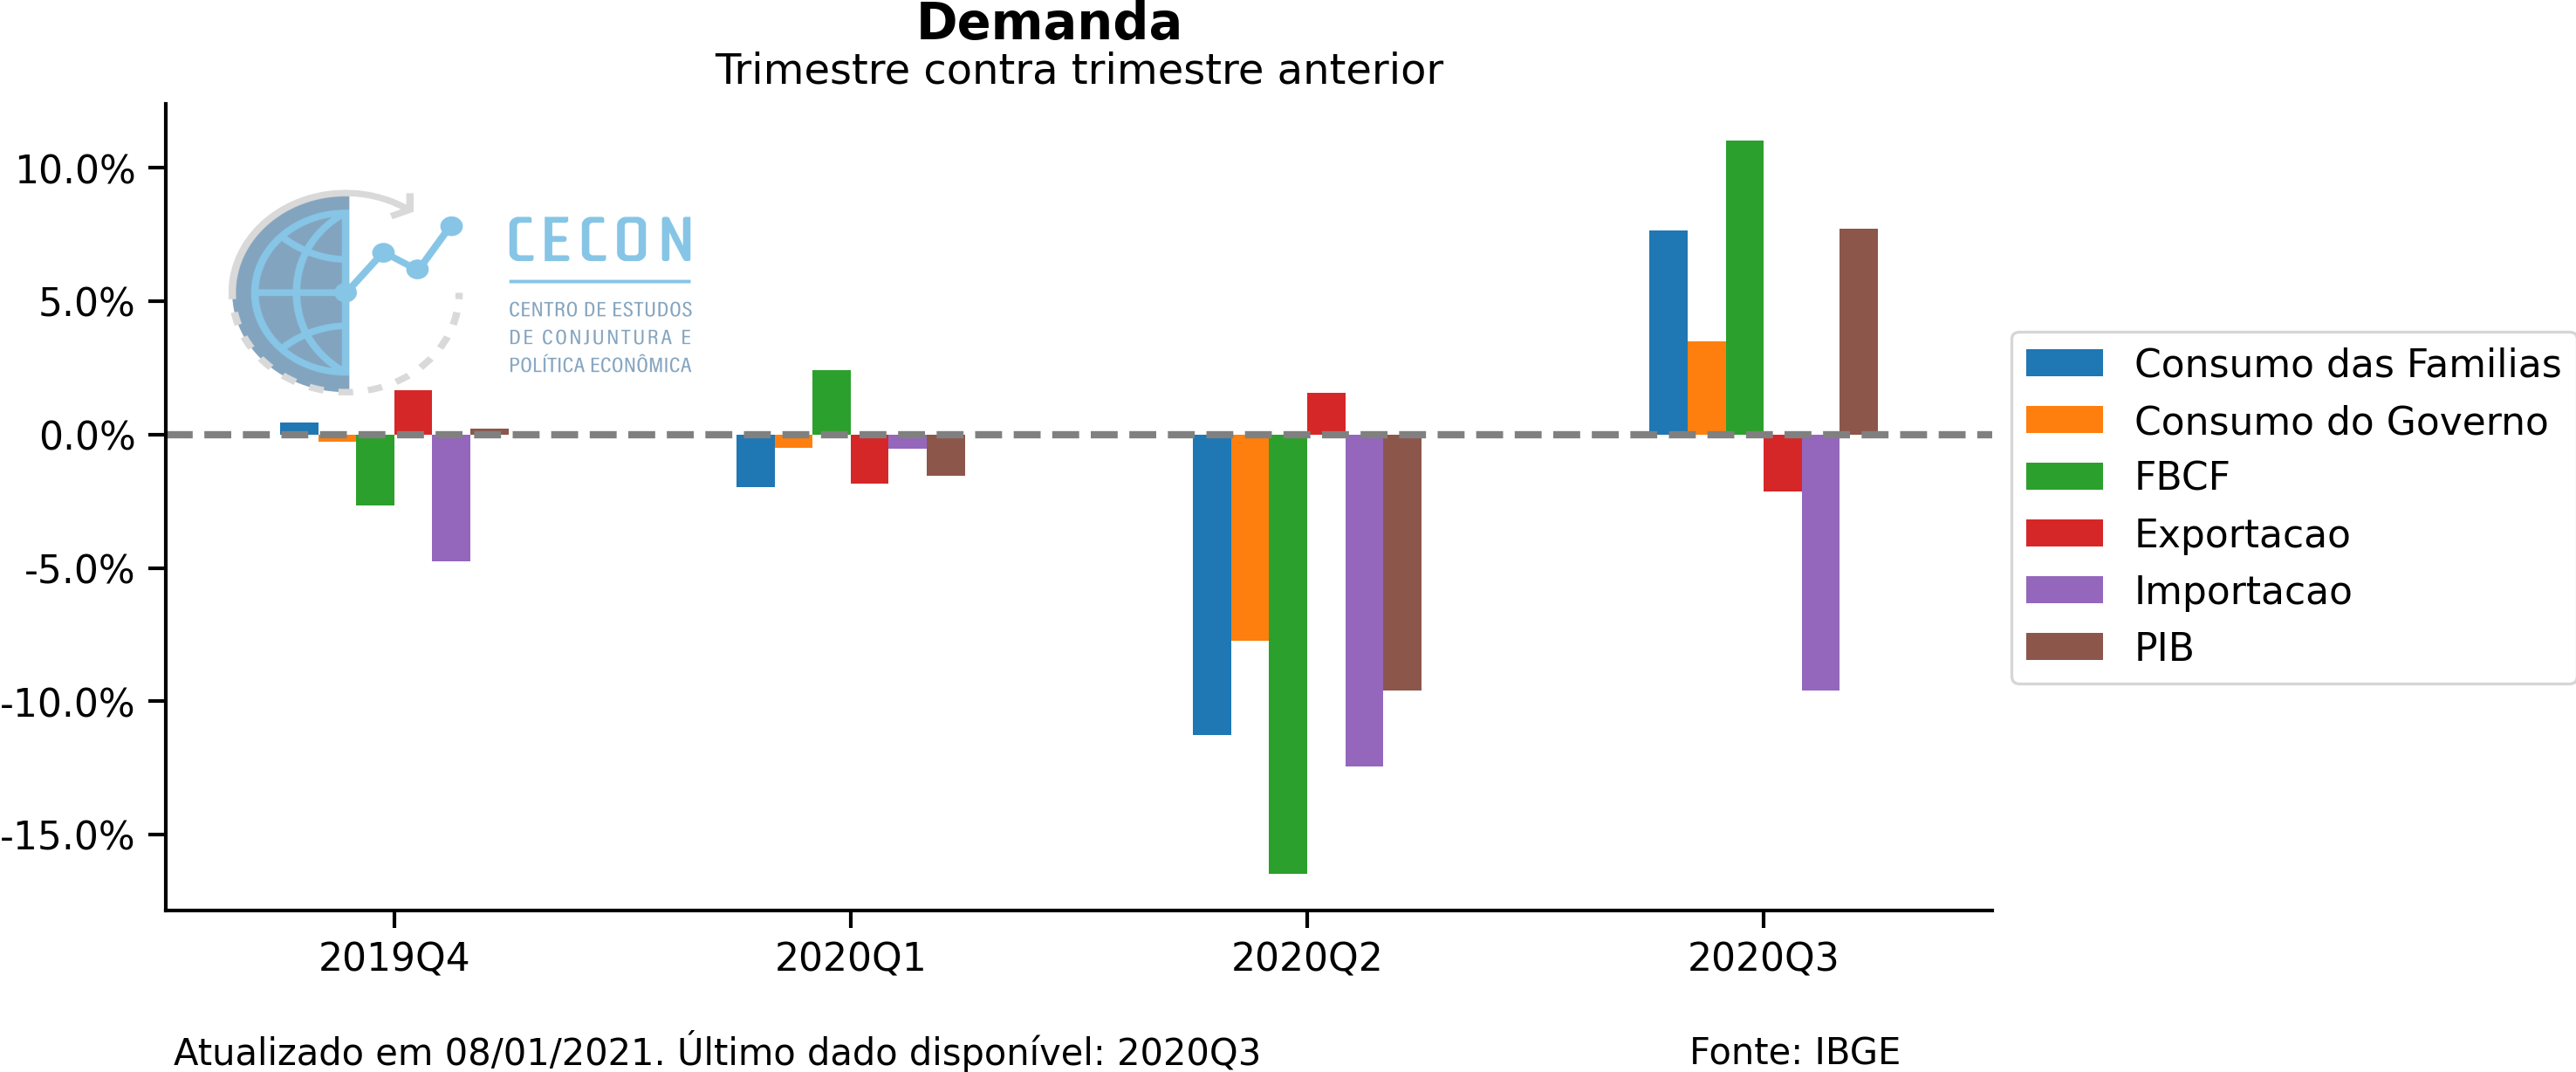
\includegraphics[width=.9\linewidth]{./figs/PIB/Demanda.png}
\end{center}

\subsection*{Oferta}
\label{sec:org11f1b72}


\begin{center}
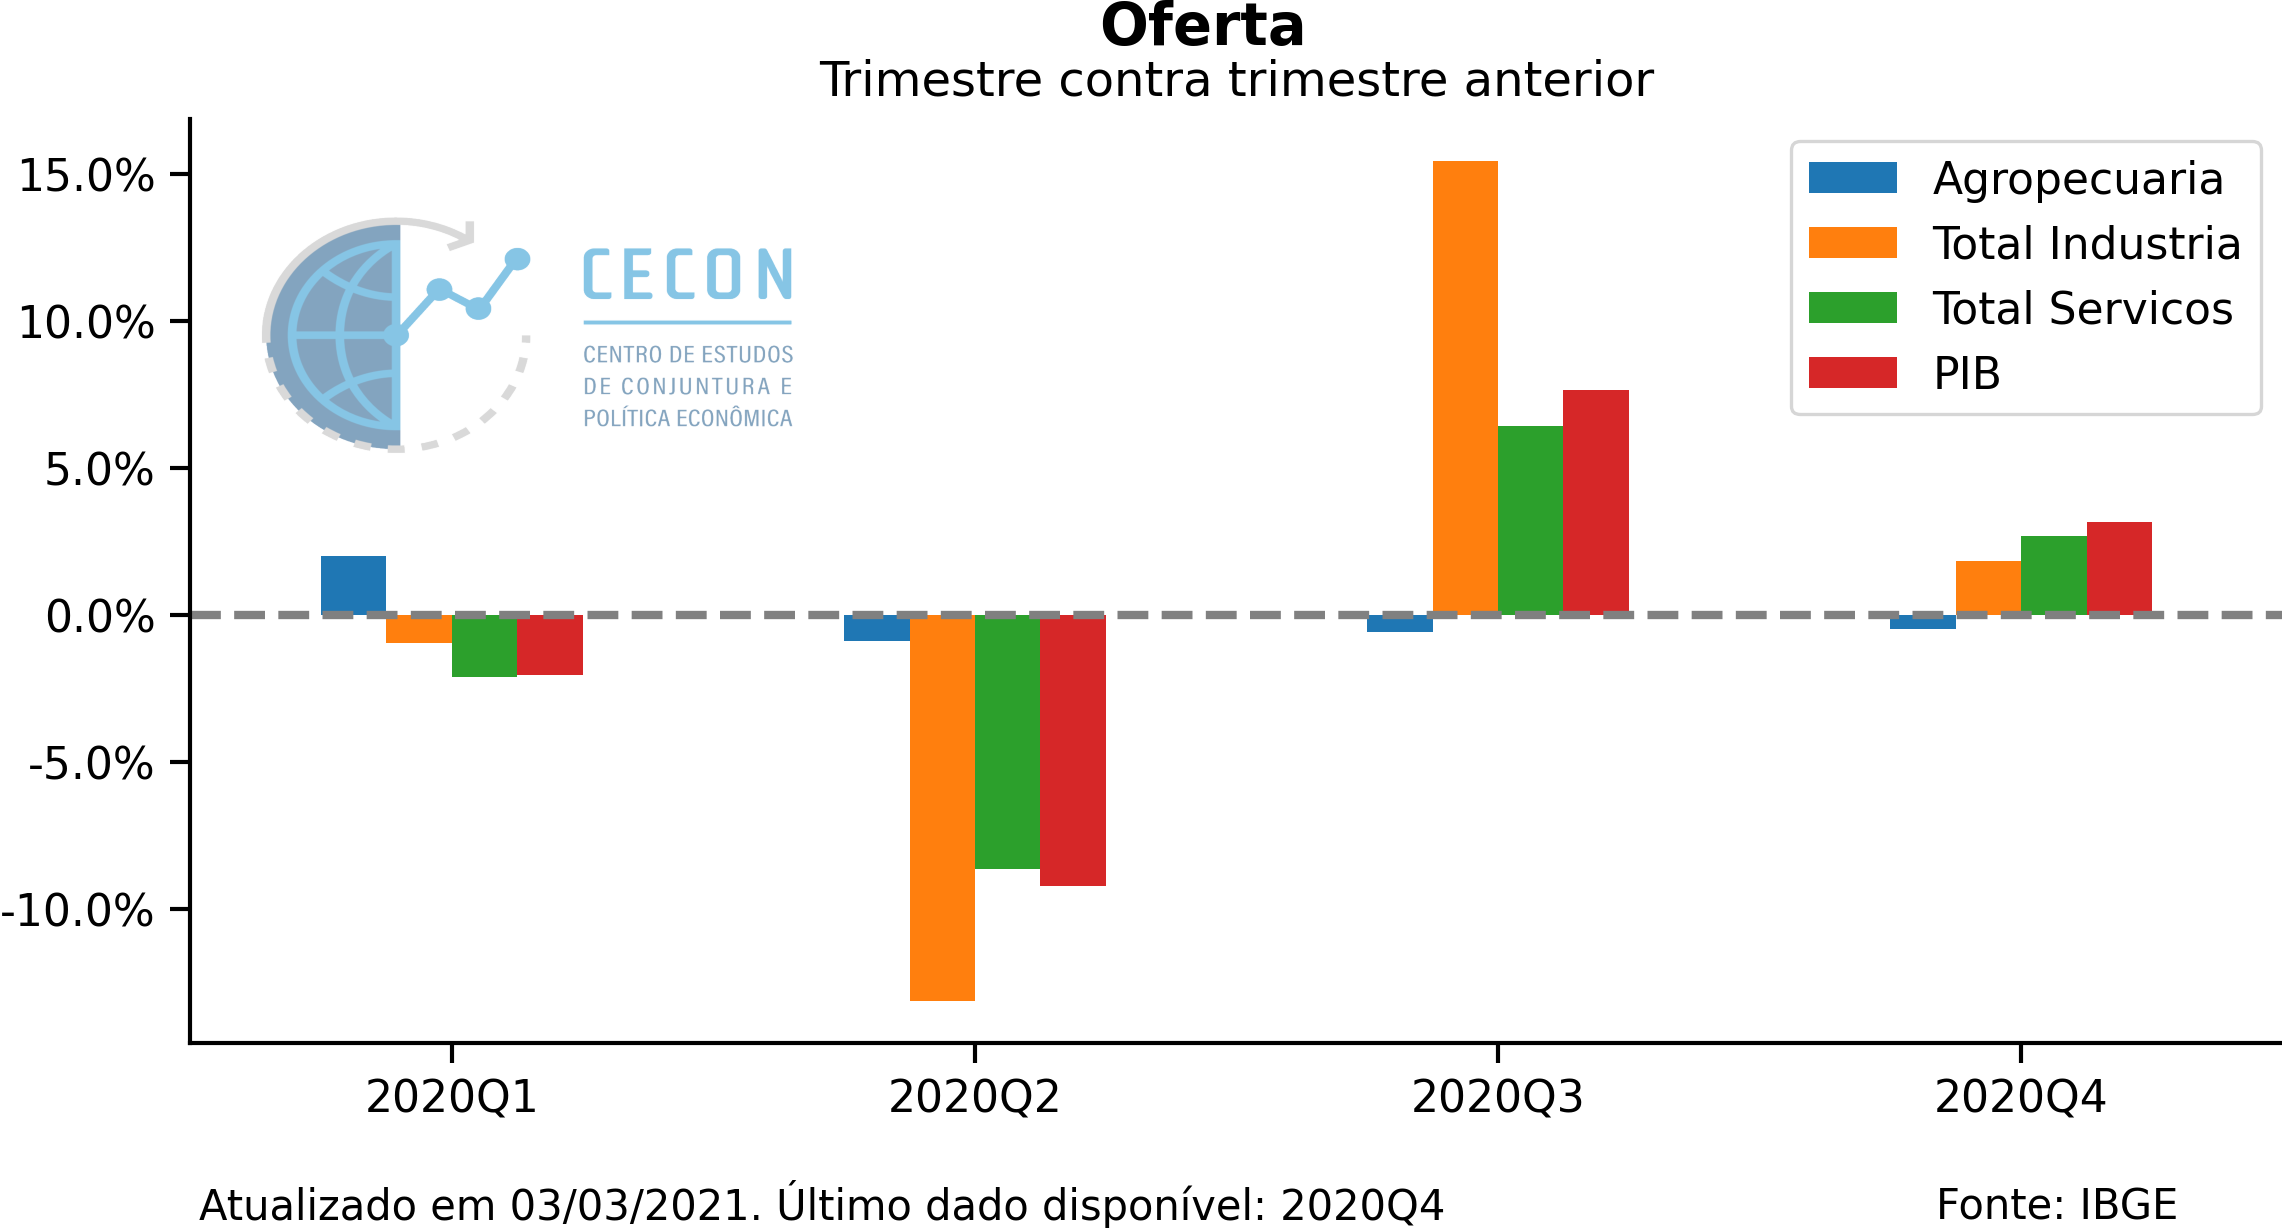
\includegraphics[width=.9\linewidth]{./figs/PIB/Oferta.png}
\end{center}


\subsection*{Contribuição para variação: Demanda}
\label{sec:orgb2575f1}

\begin{center}
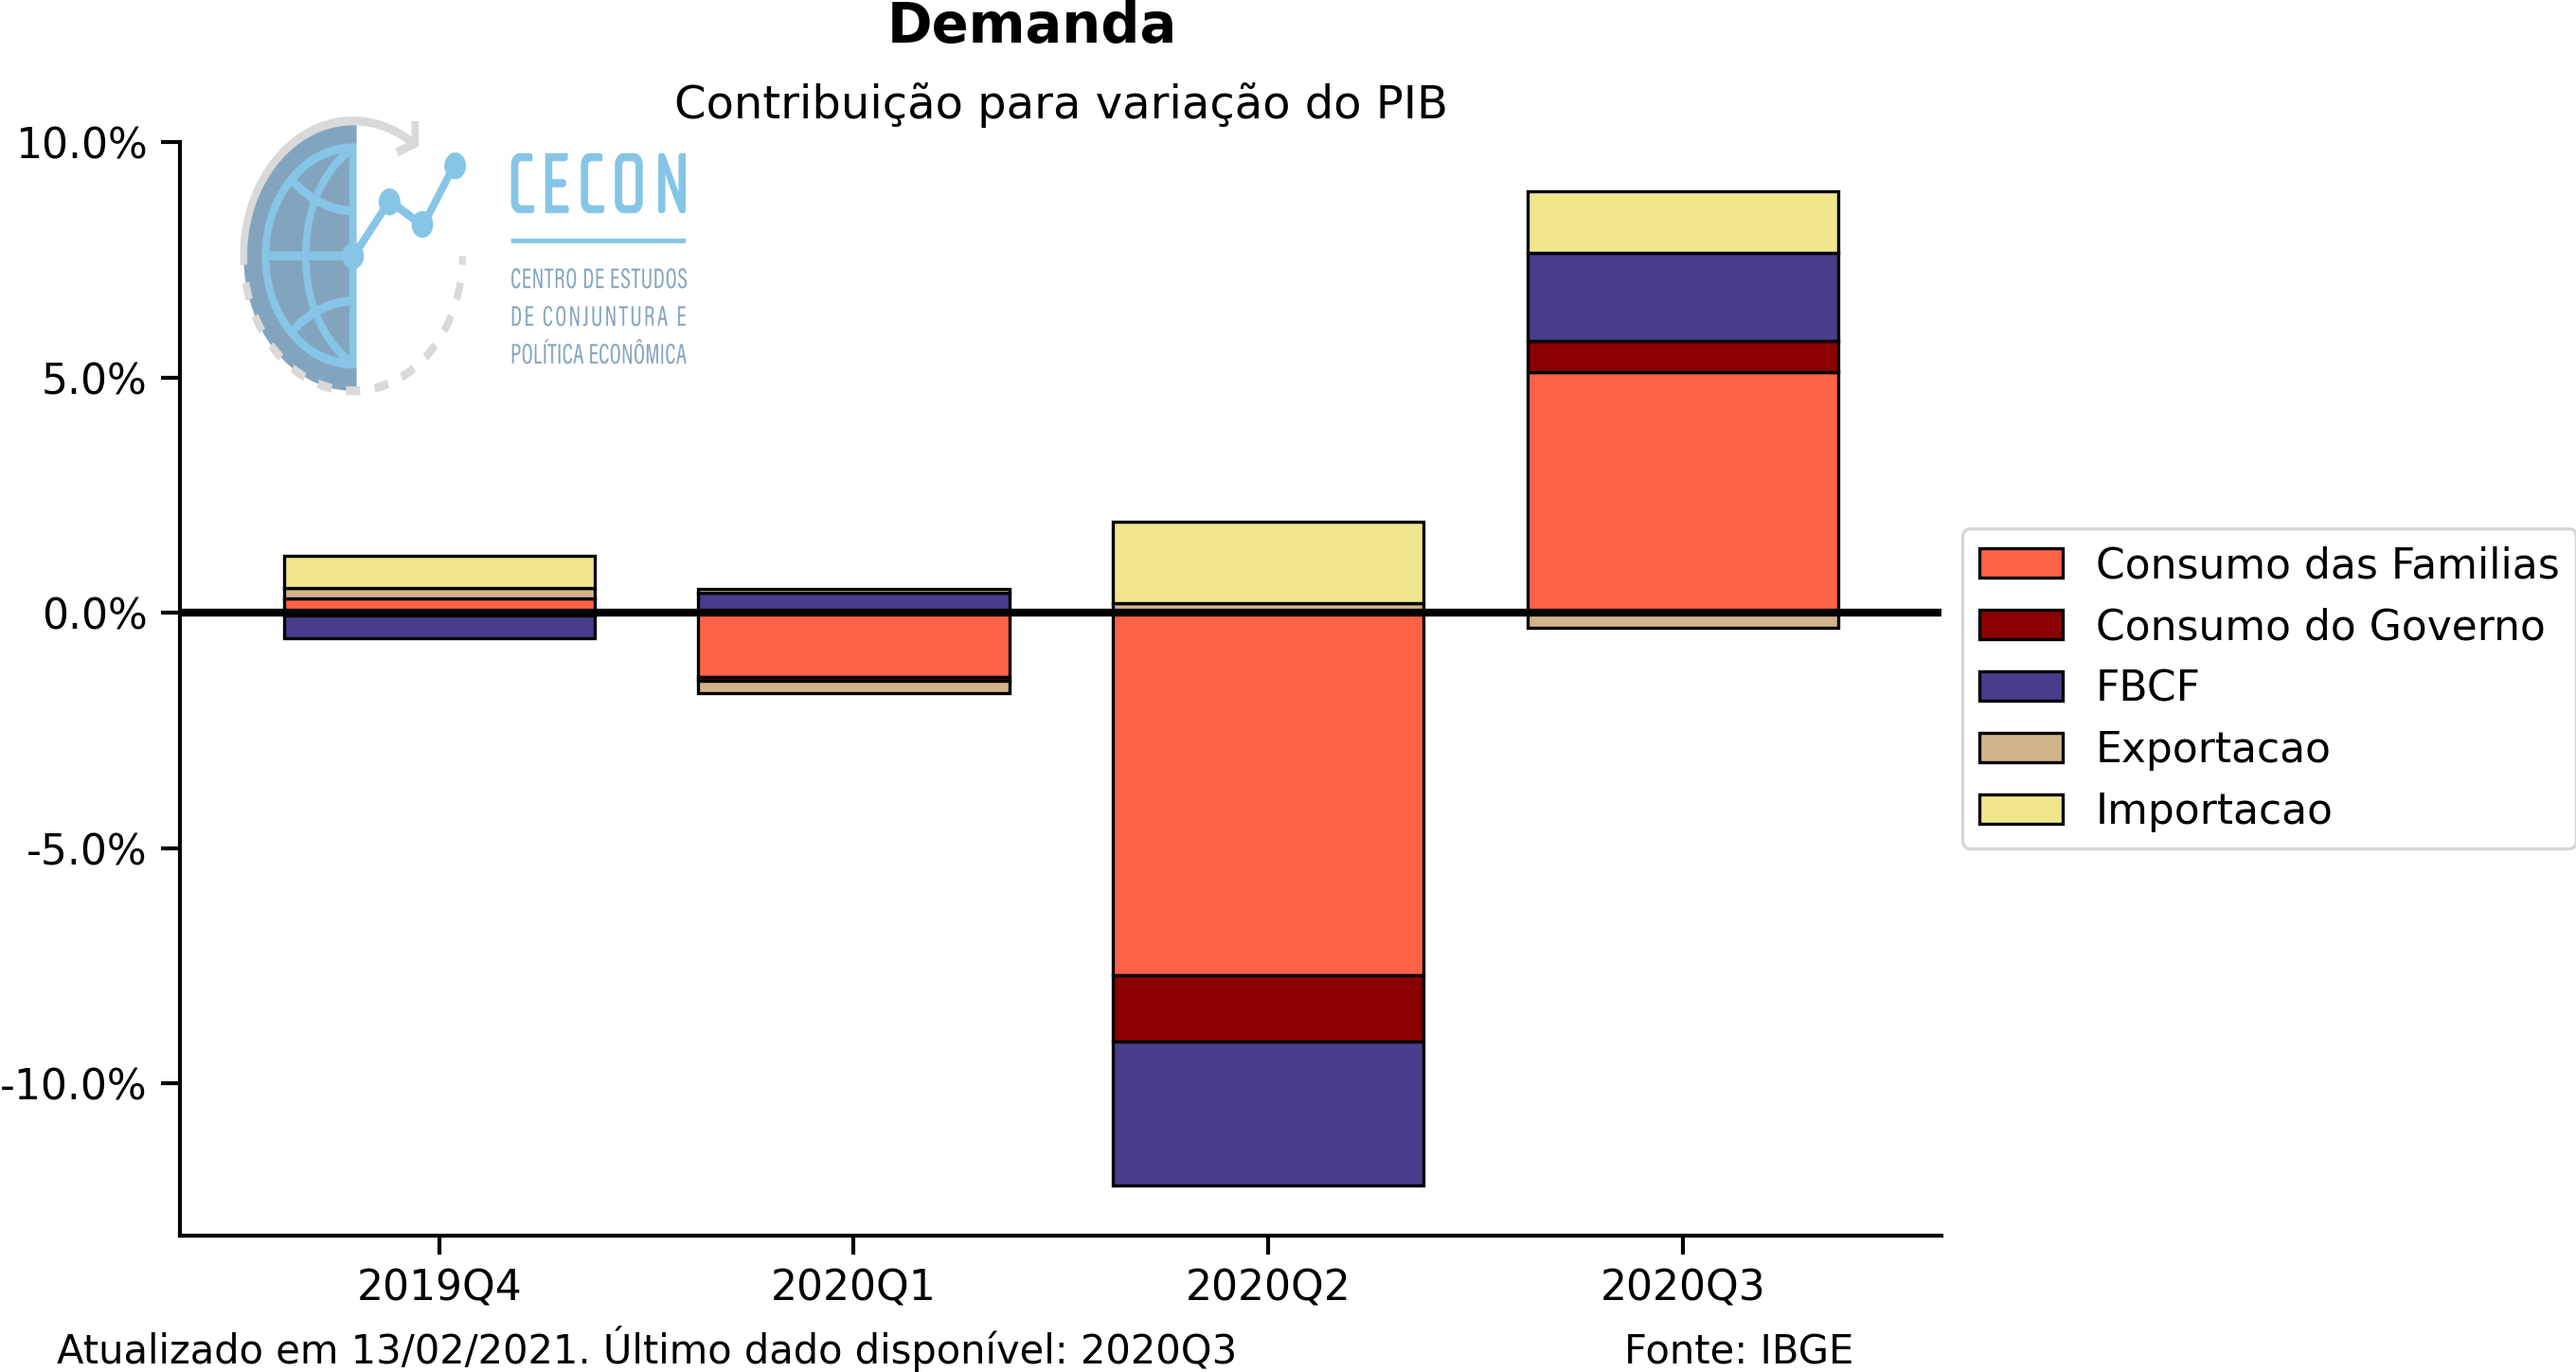
\includegraphics[width=.9\linewidth]{./figs/PIB/Contrib_Demanda.png}
\end{center}

\subsection*{Contribuição para variação: Oferta}
\label{sec:org110ff1f}

\begin{center}
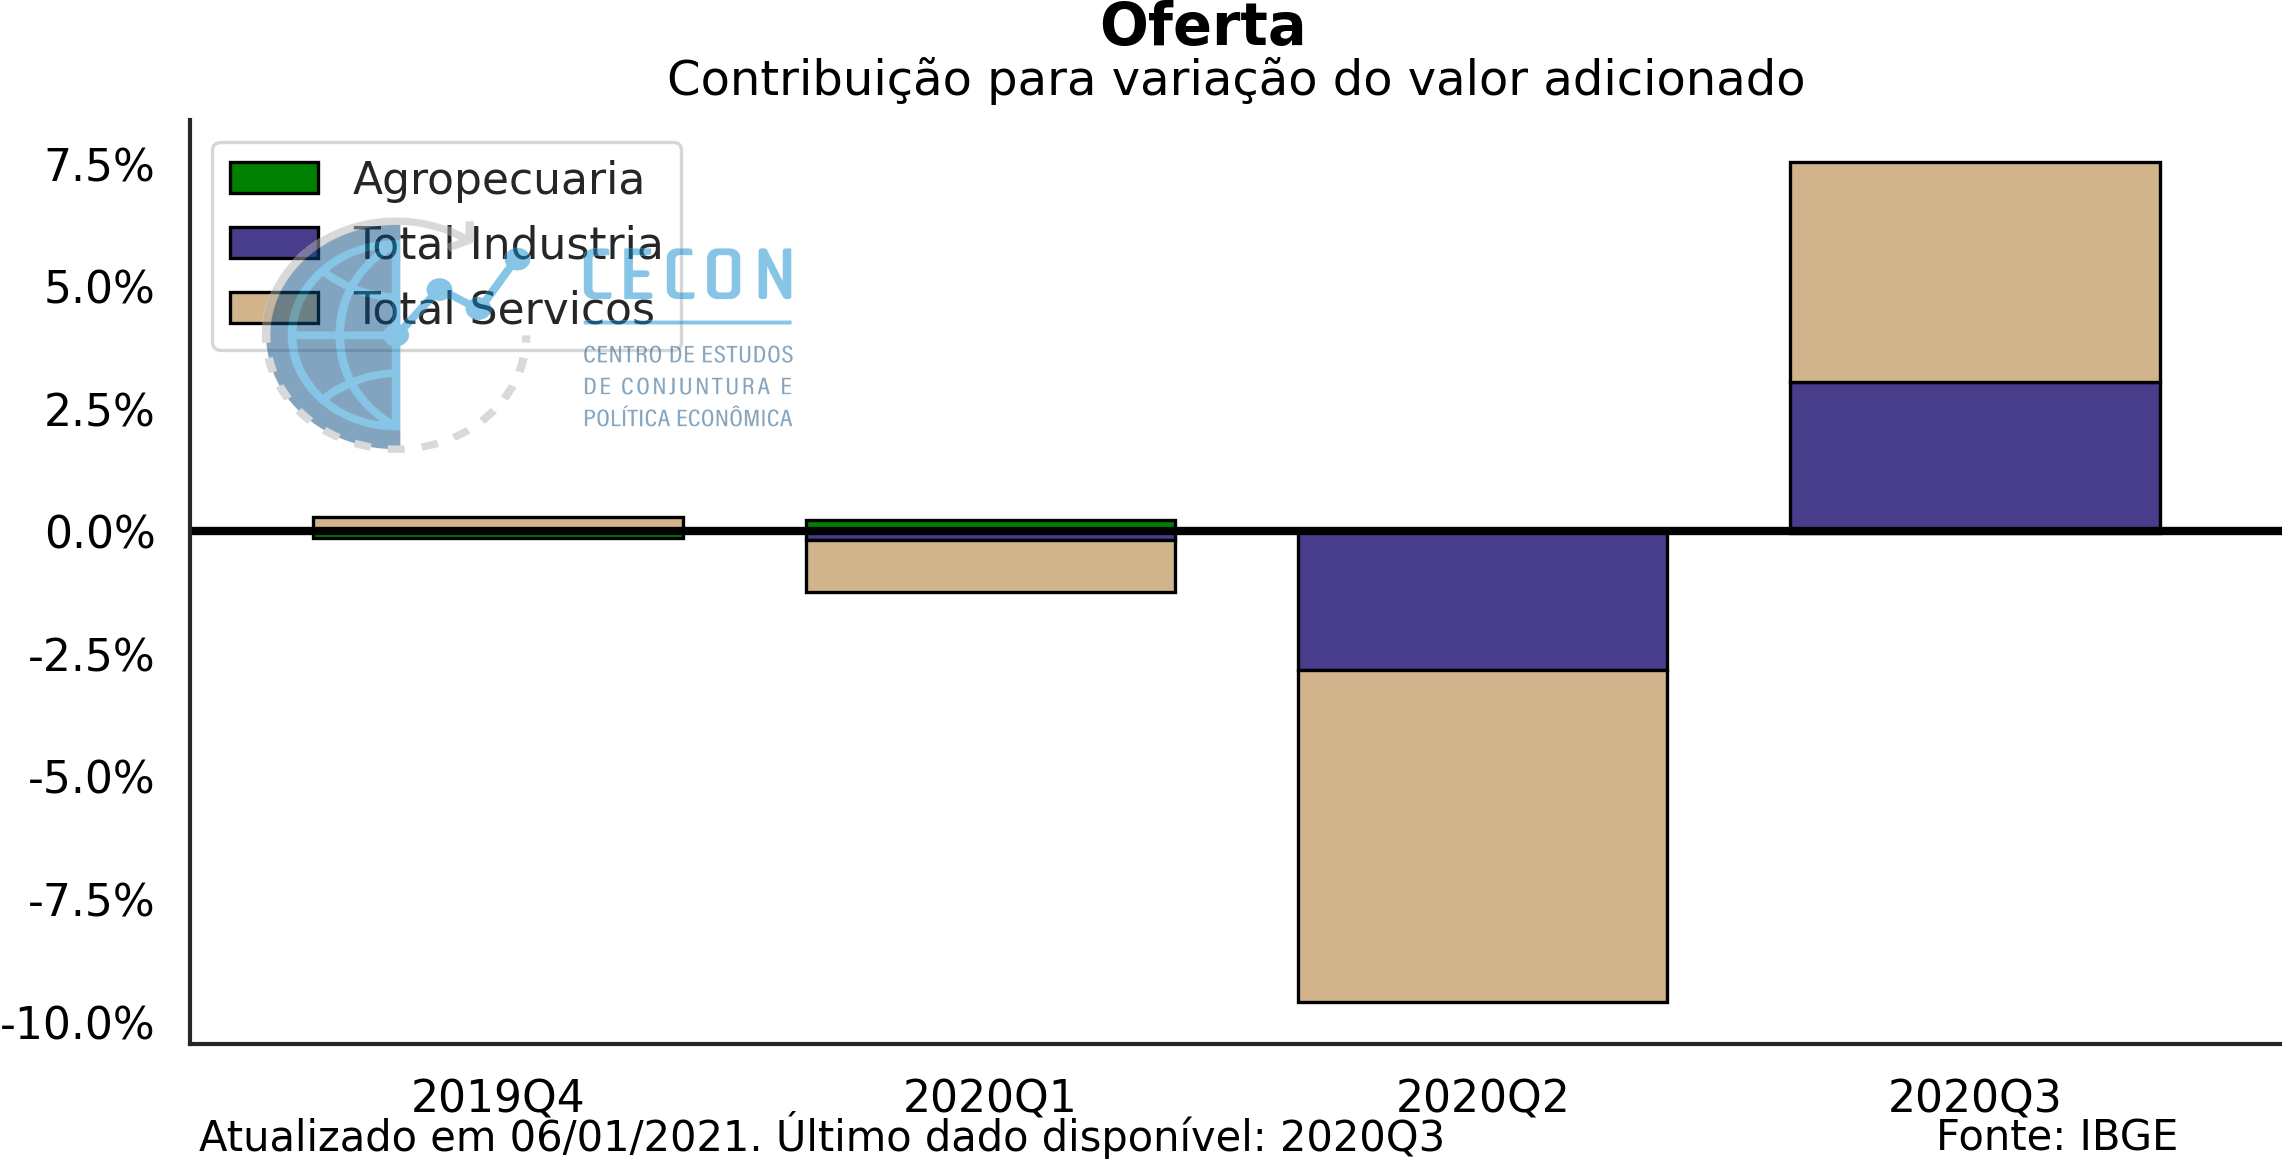
\includegraphics[width=.9\linewidth]{./figs/PIB/Contrib_Oferta.png}
\end{center}


\subsection*{Contribuição para variação: Serviços}
\label{sec:org8e1bff9}

\begin{center}
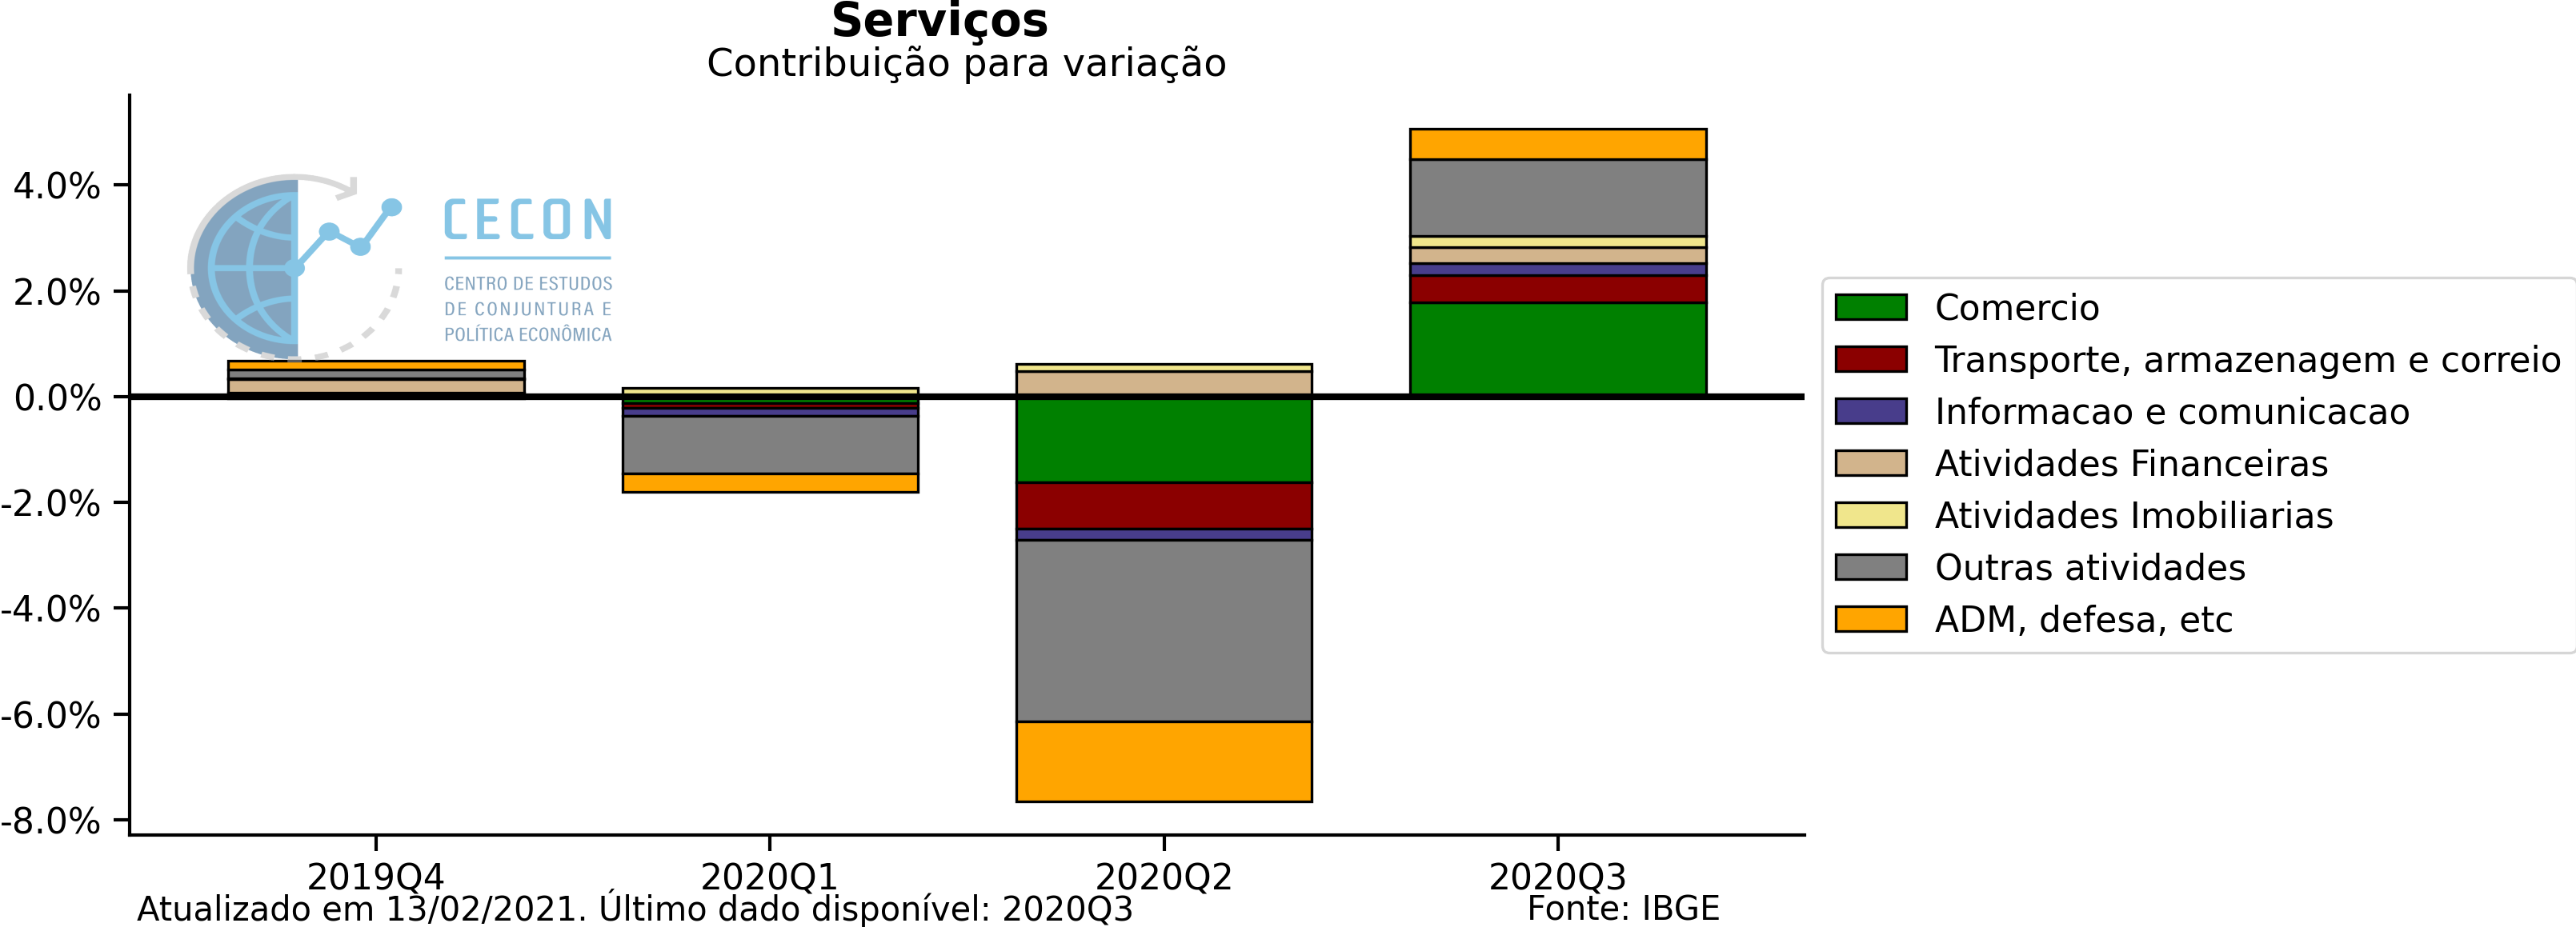
\includegraphics[width=.9\linewidth]{./figs/PIB/Contrib_Servicos.png}
\end{center}

\section*{Crédito}
\label{sec:org1fe3f9f}

\subsection*{Endividamento das famílias}
\label{sec:orgd486013}

\begin{center}
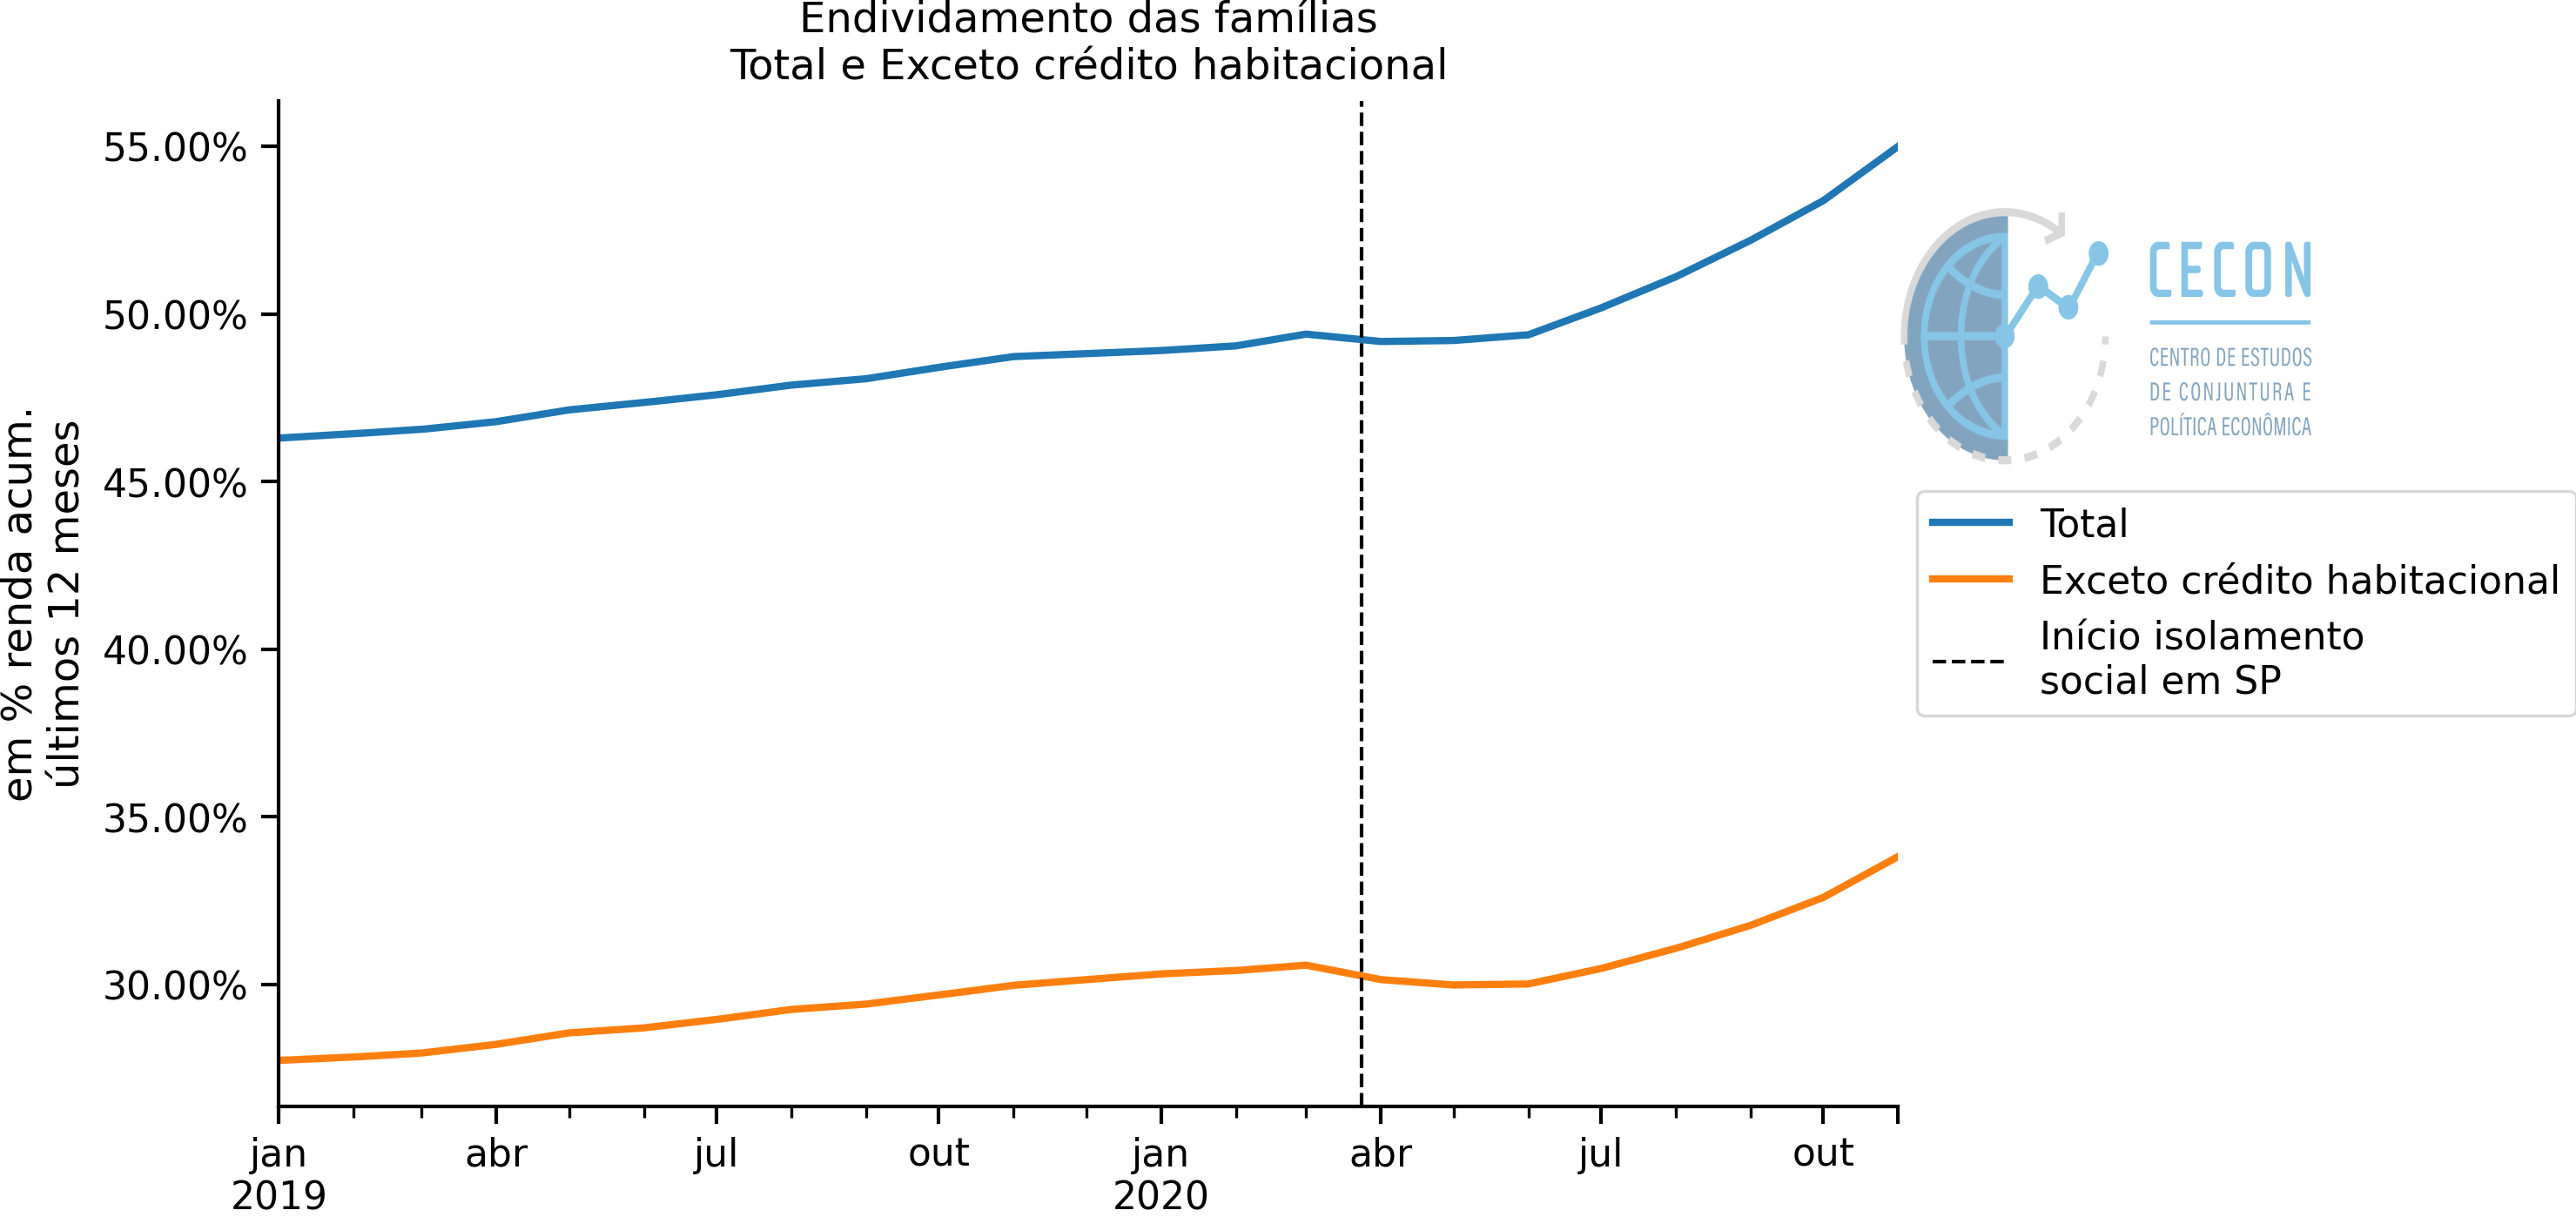
\includegraphics[width=.9\linewidth]{./figs/Credito/EndividamentoFamilias.png}
\end{center}


\subsection*{Saldo Pessoal Jurídica - Nível}
\label{sec:orgf8b1899}

\begin{center}
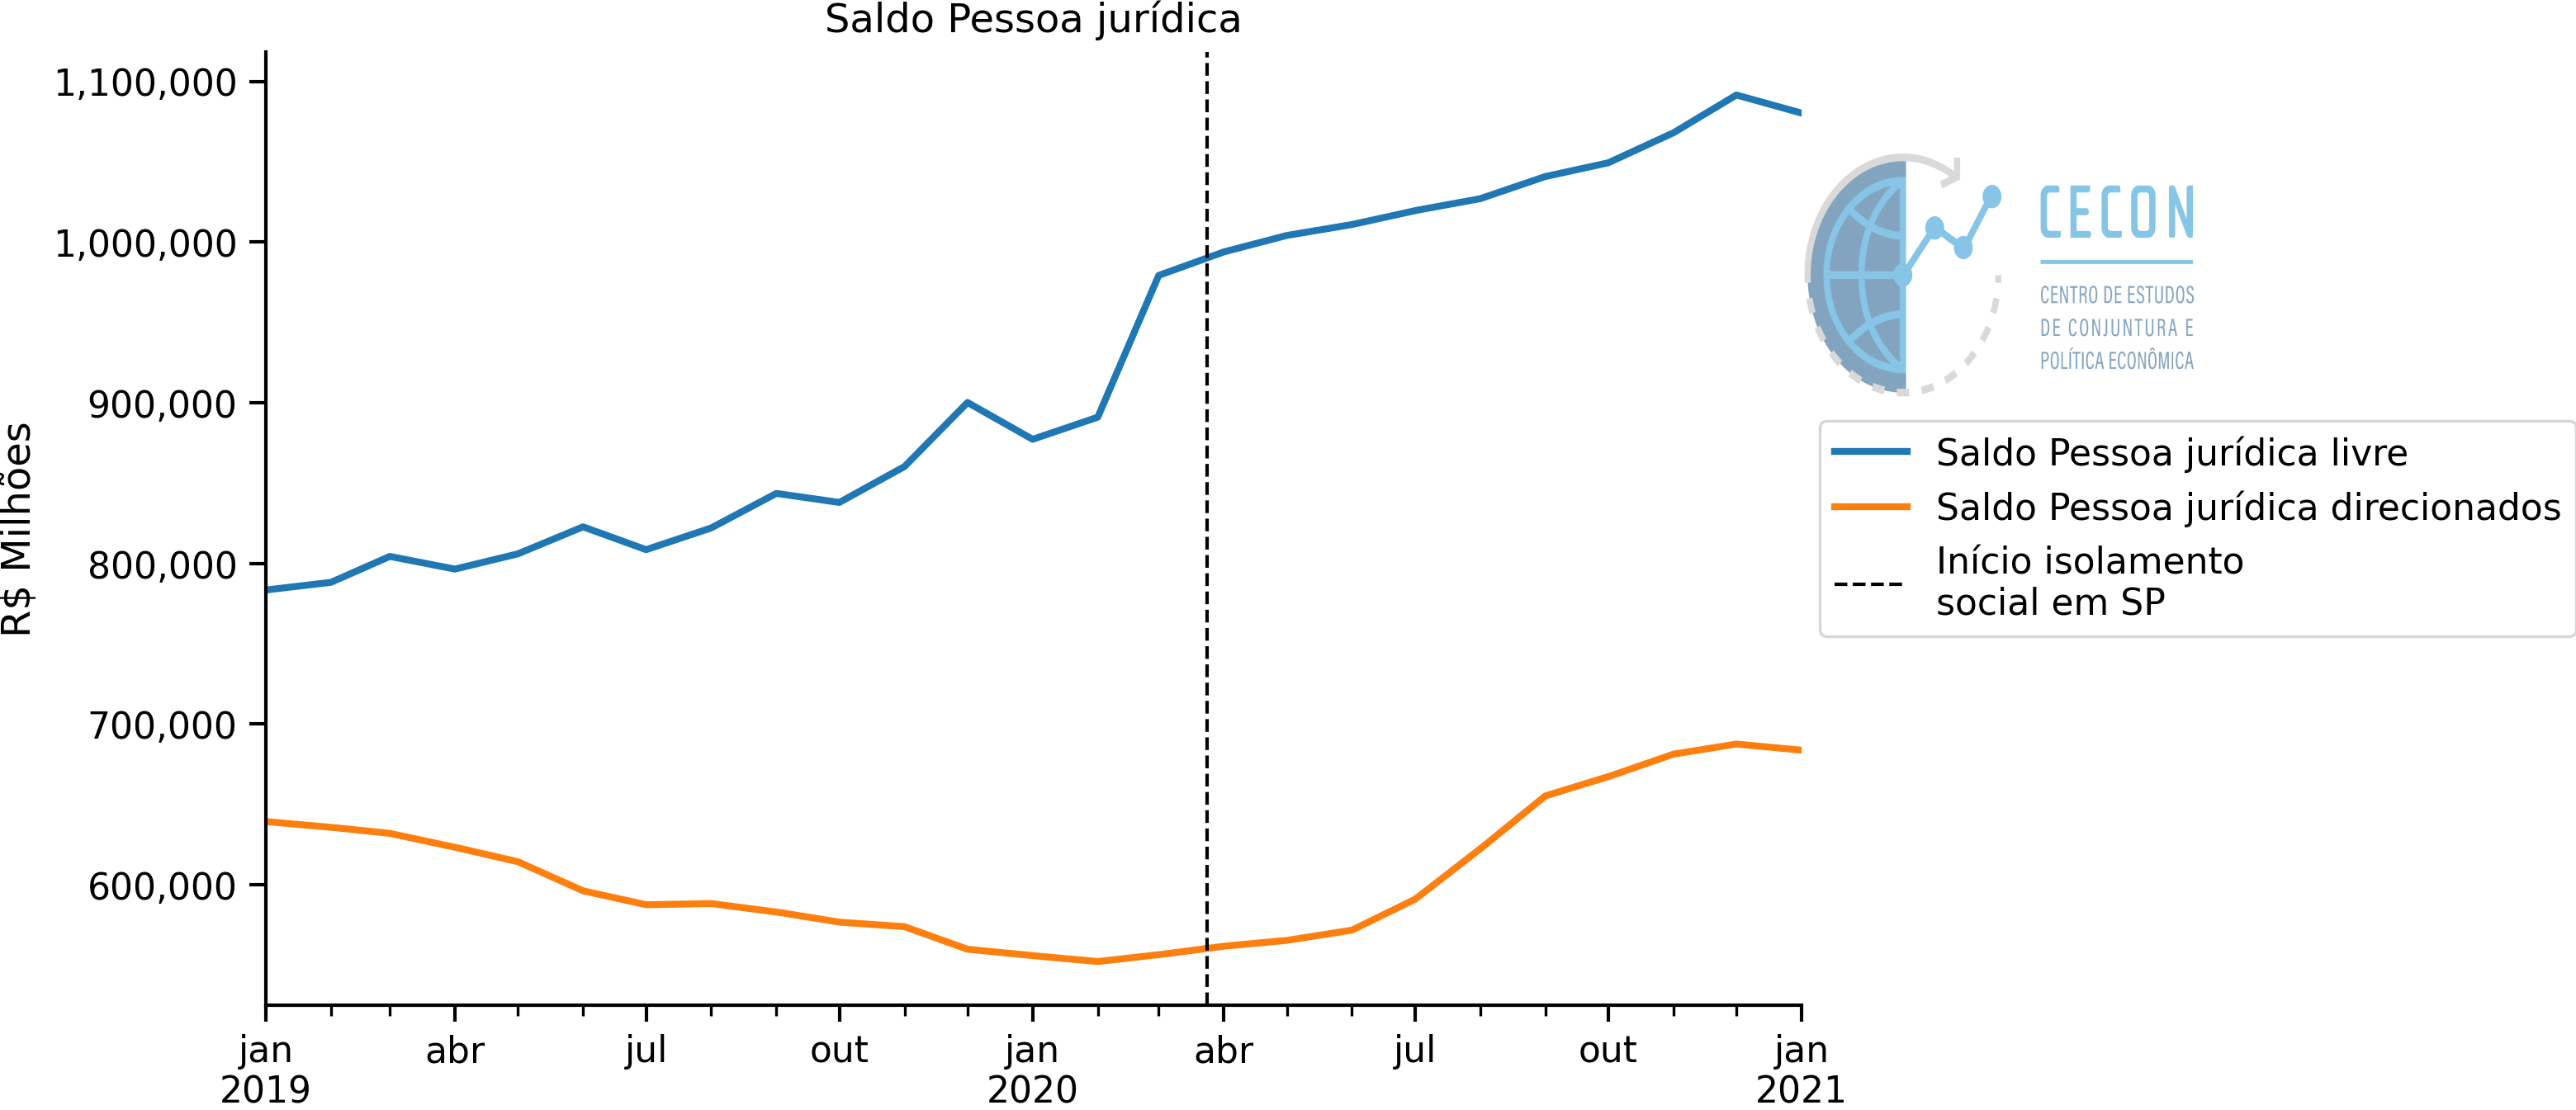
\includegraphics[width=.9\linewidth]{./figs/Credito/SaldoPJ.png}
\end{center}



\subsection*{Saldo Pessoa Jurídica - em \% do PIB}
\label{sec:orge5e21be}
\begin{center}
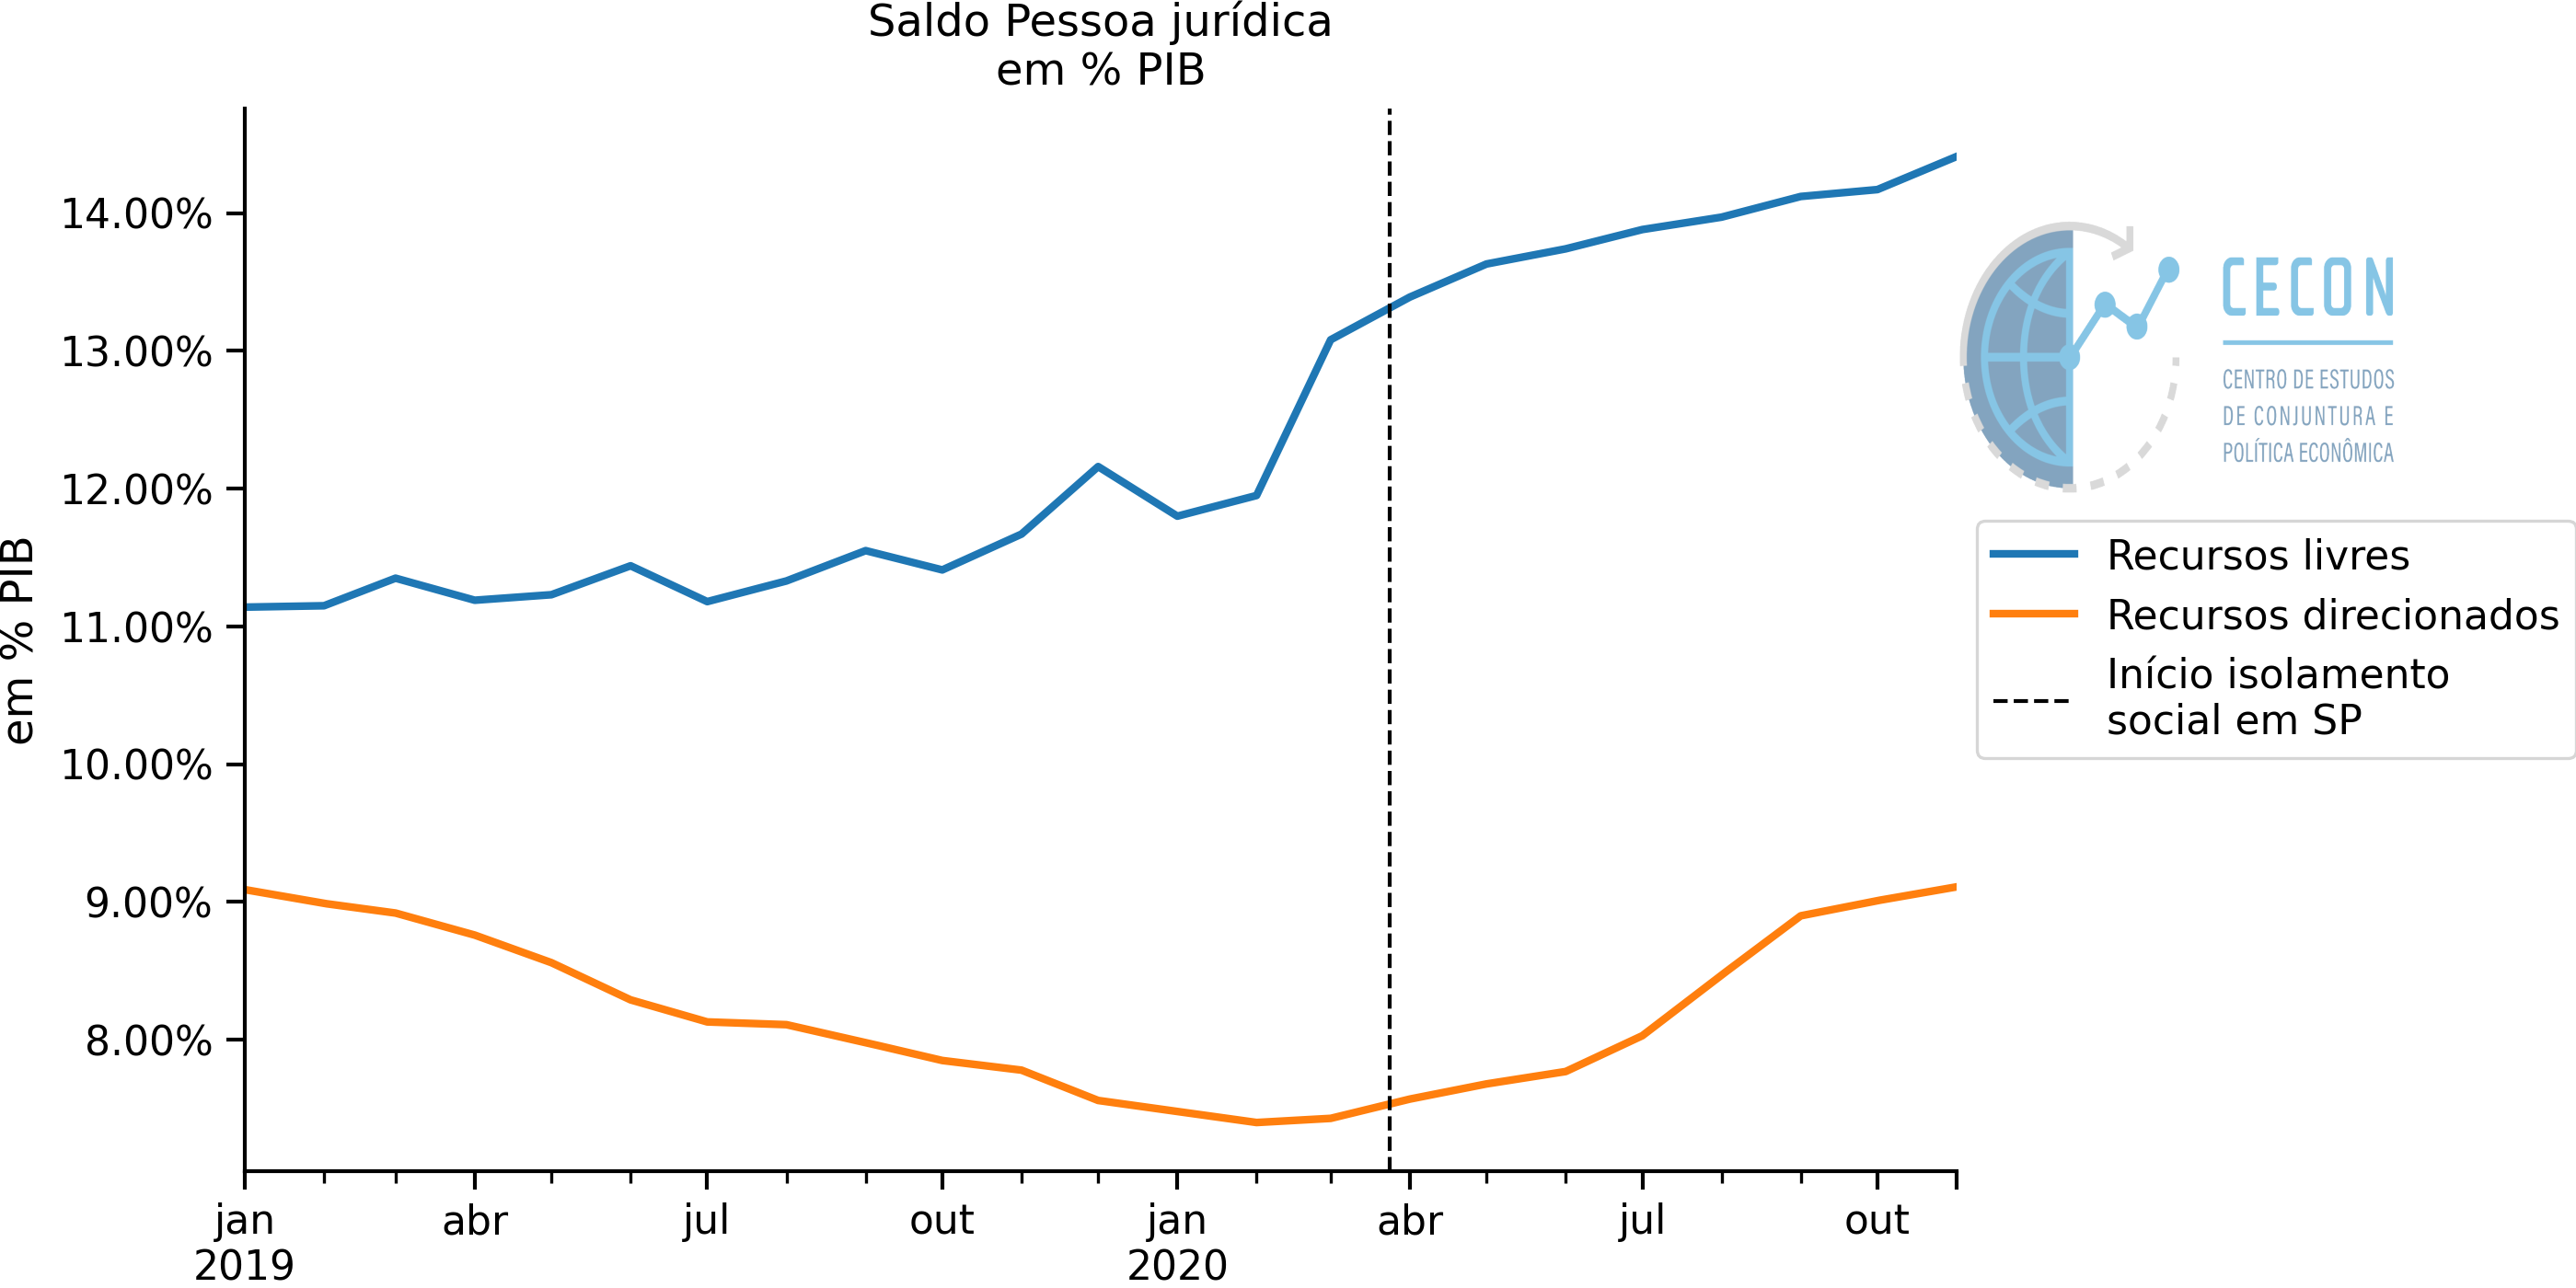
\includegraphics[width=.9\linewidth]{./figs/Credito/SaldoPJ_PIB.png}
\end{center}

\subsection*{Saldo Pessoa física - Nível}
\label{sec:orgf013576}

\begin{center}
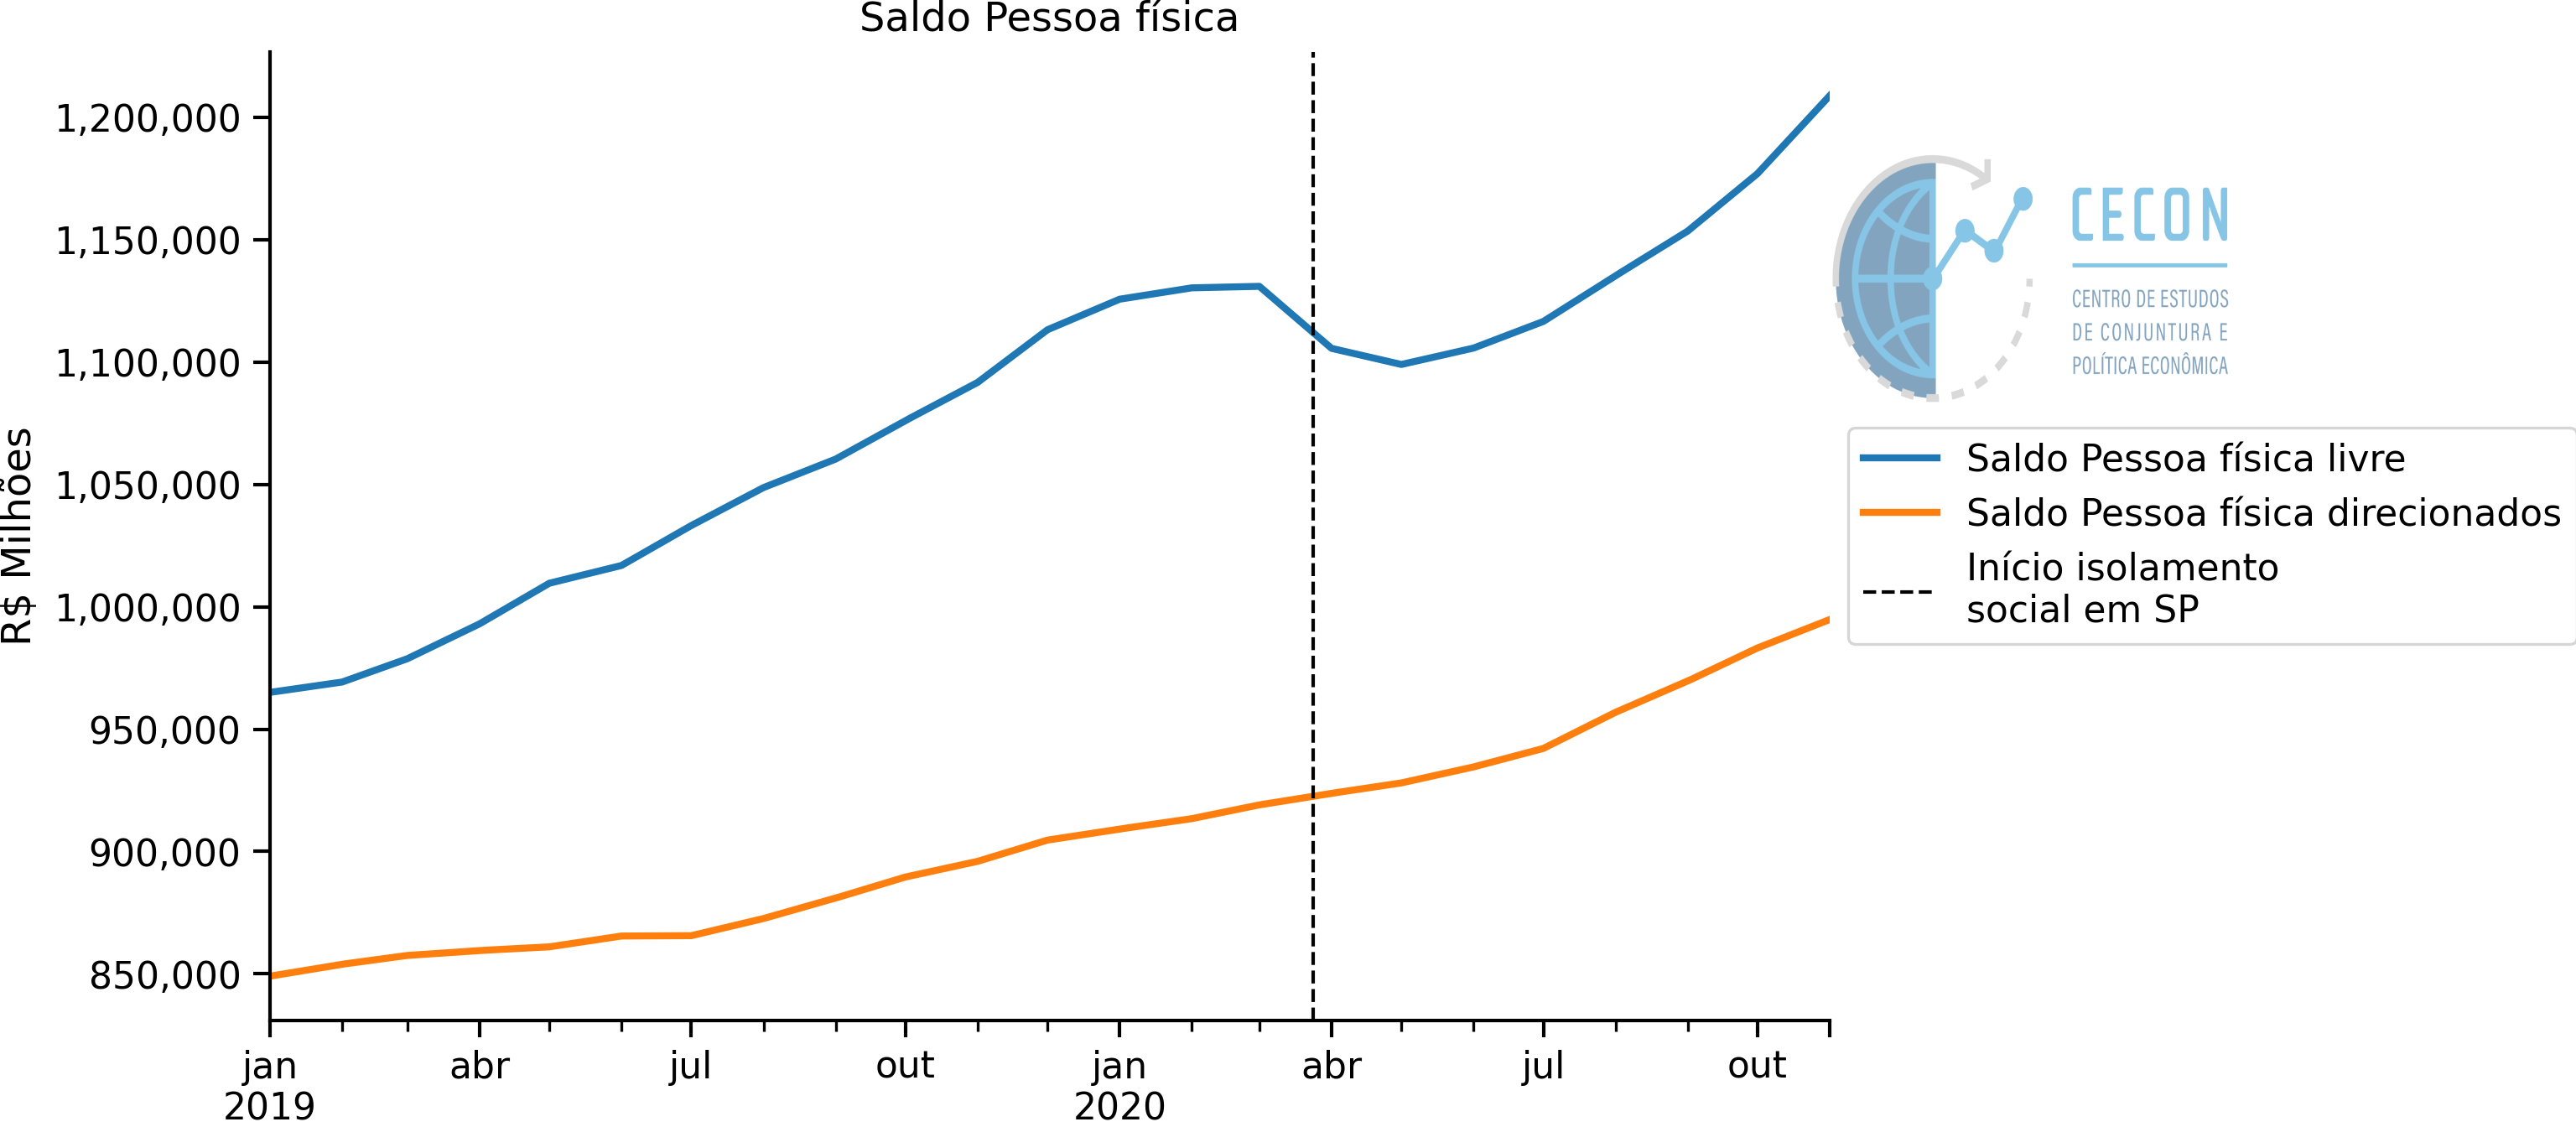
\includegraphics[width=.9\linewidth]{./figs/Credito/SaldoPF.png}
\end{center}


\subsection*{Saldo Pessoa física - em \% do PIB}
\label{sec:org71fabaa}

\begin{center}
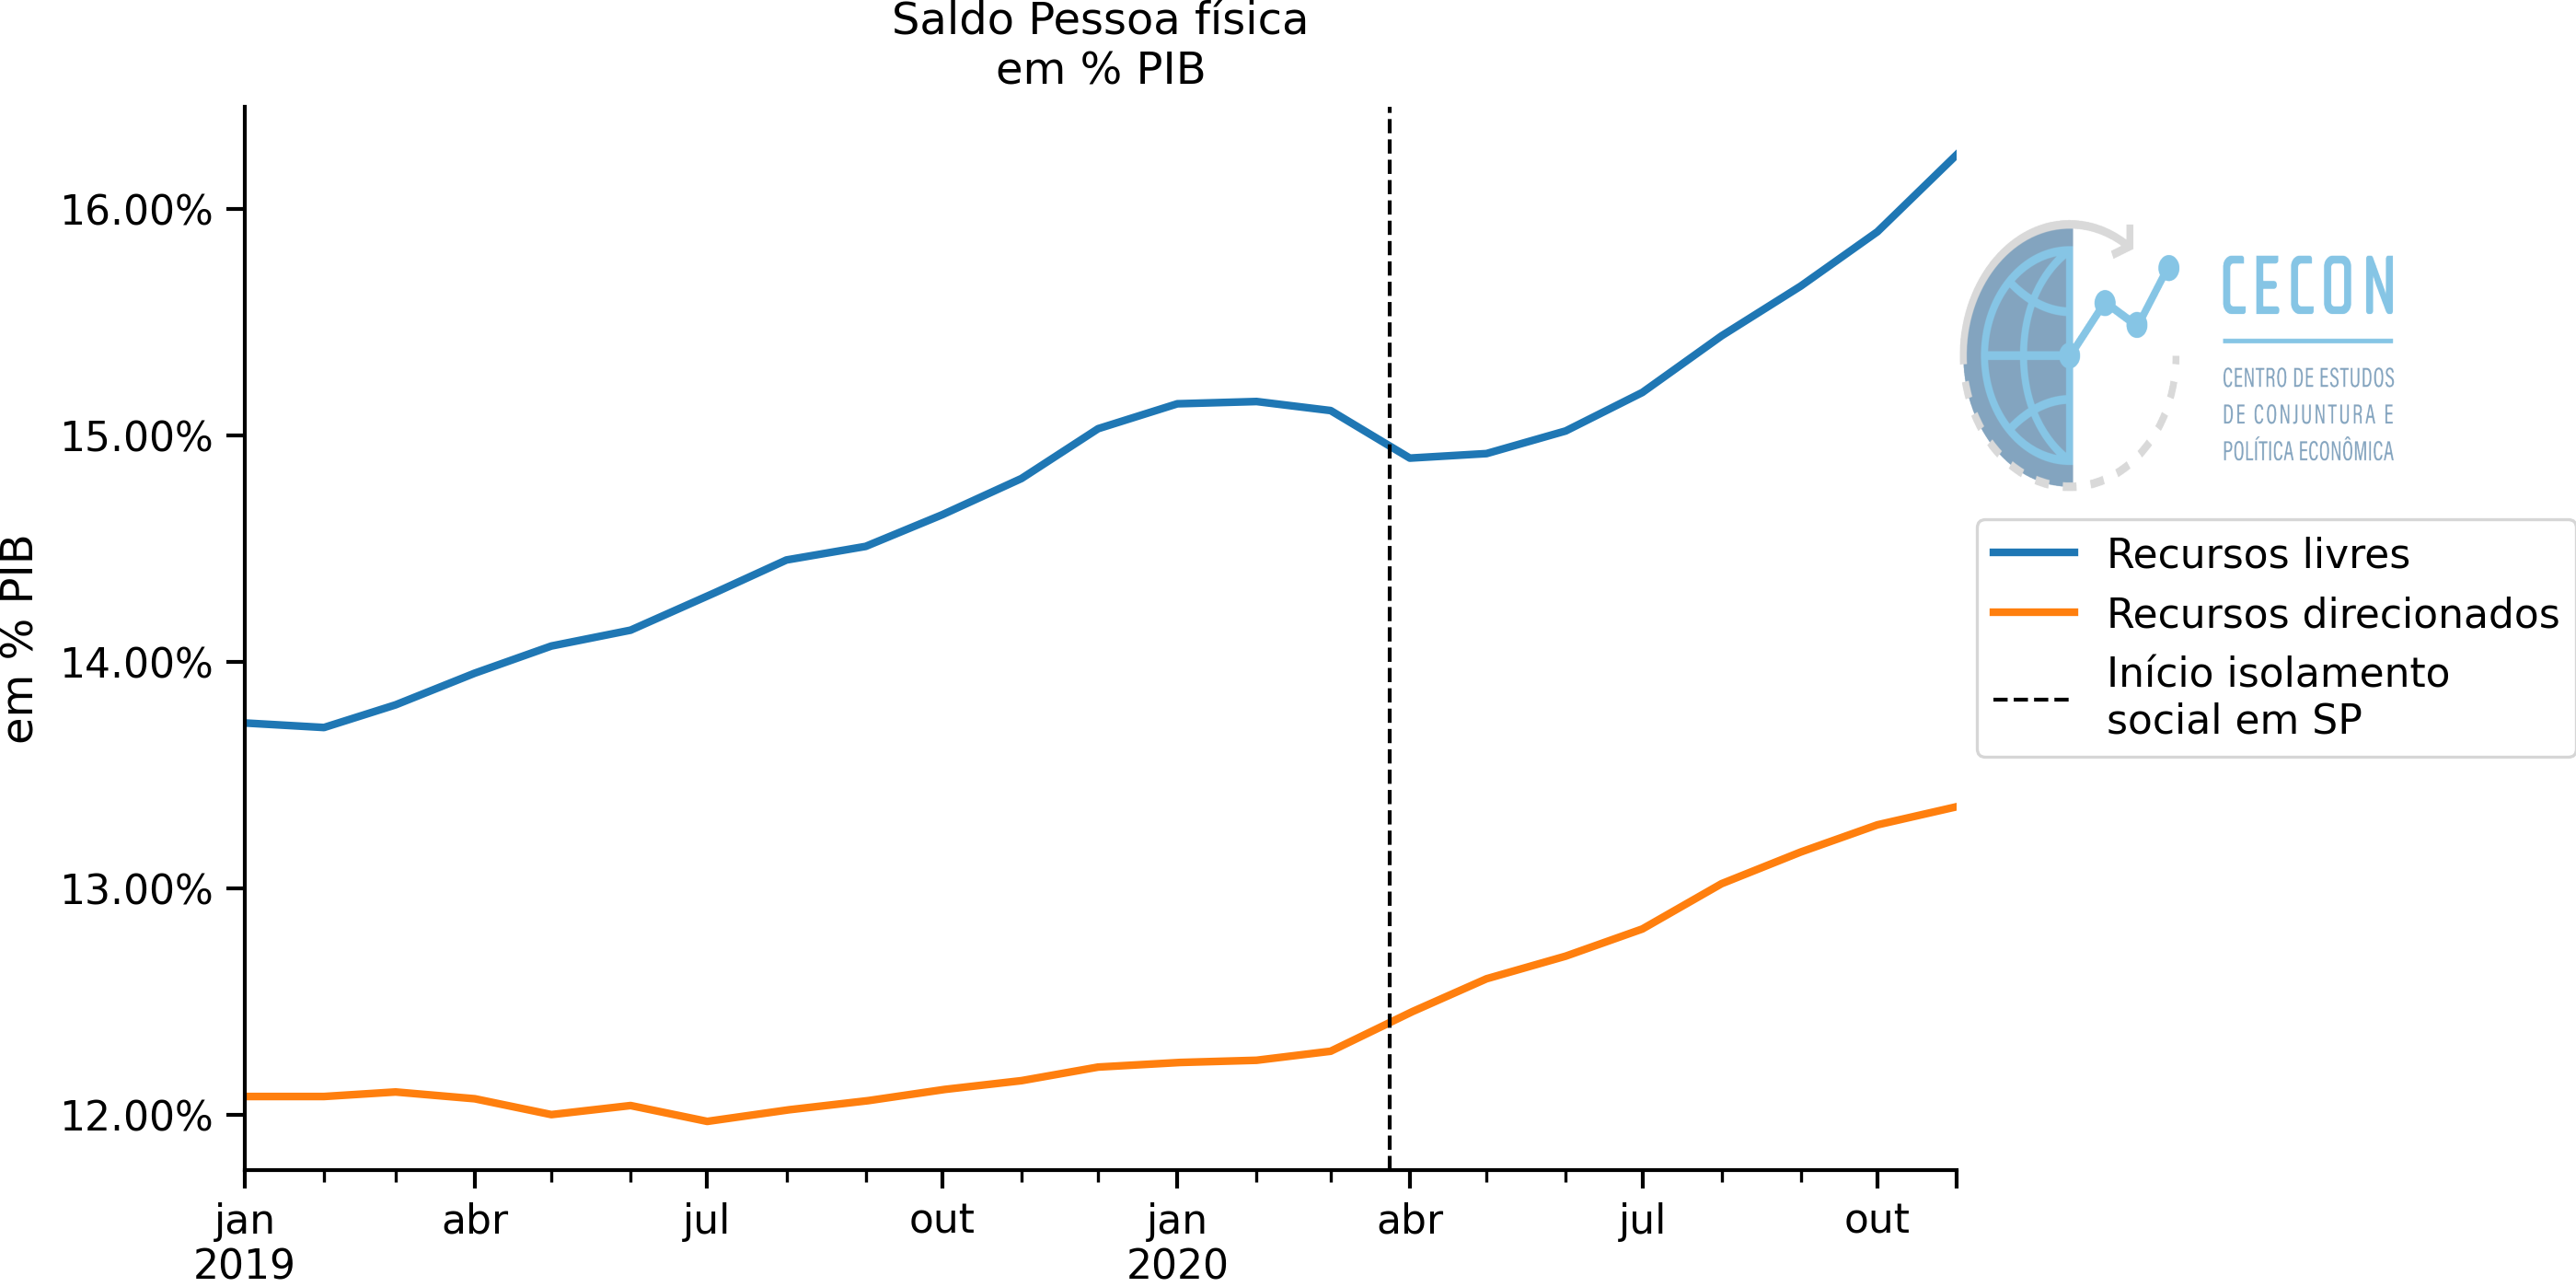
\includegraphics[width=.9\linewidth]{./figs/Credito/SaldoPF_PIB.png}
\end{center}


\subsection*{Crédito ampliado em \% do Total}
\label{sec:orga6cfeca}

\begin{center}
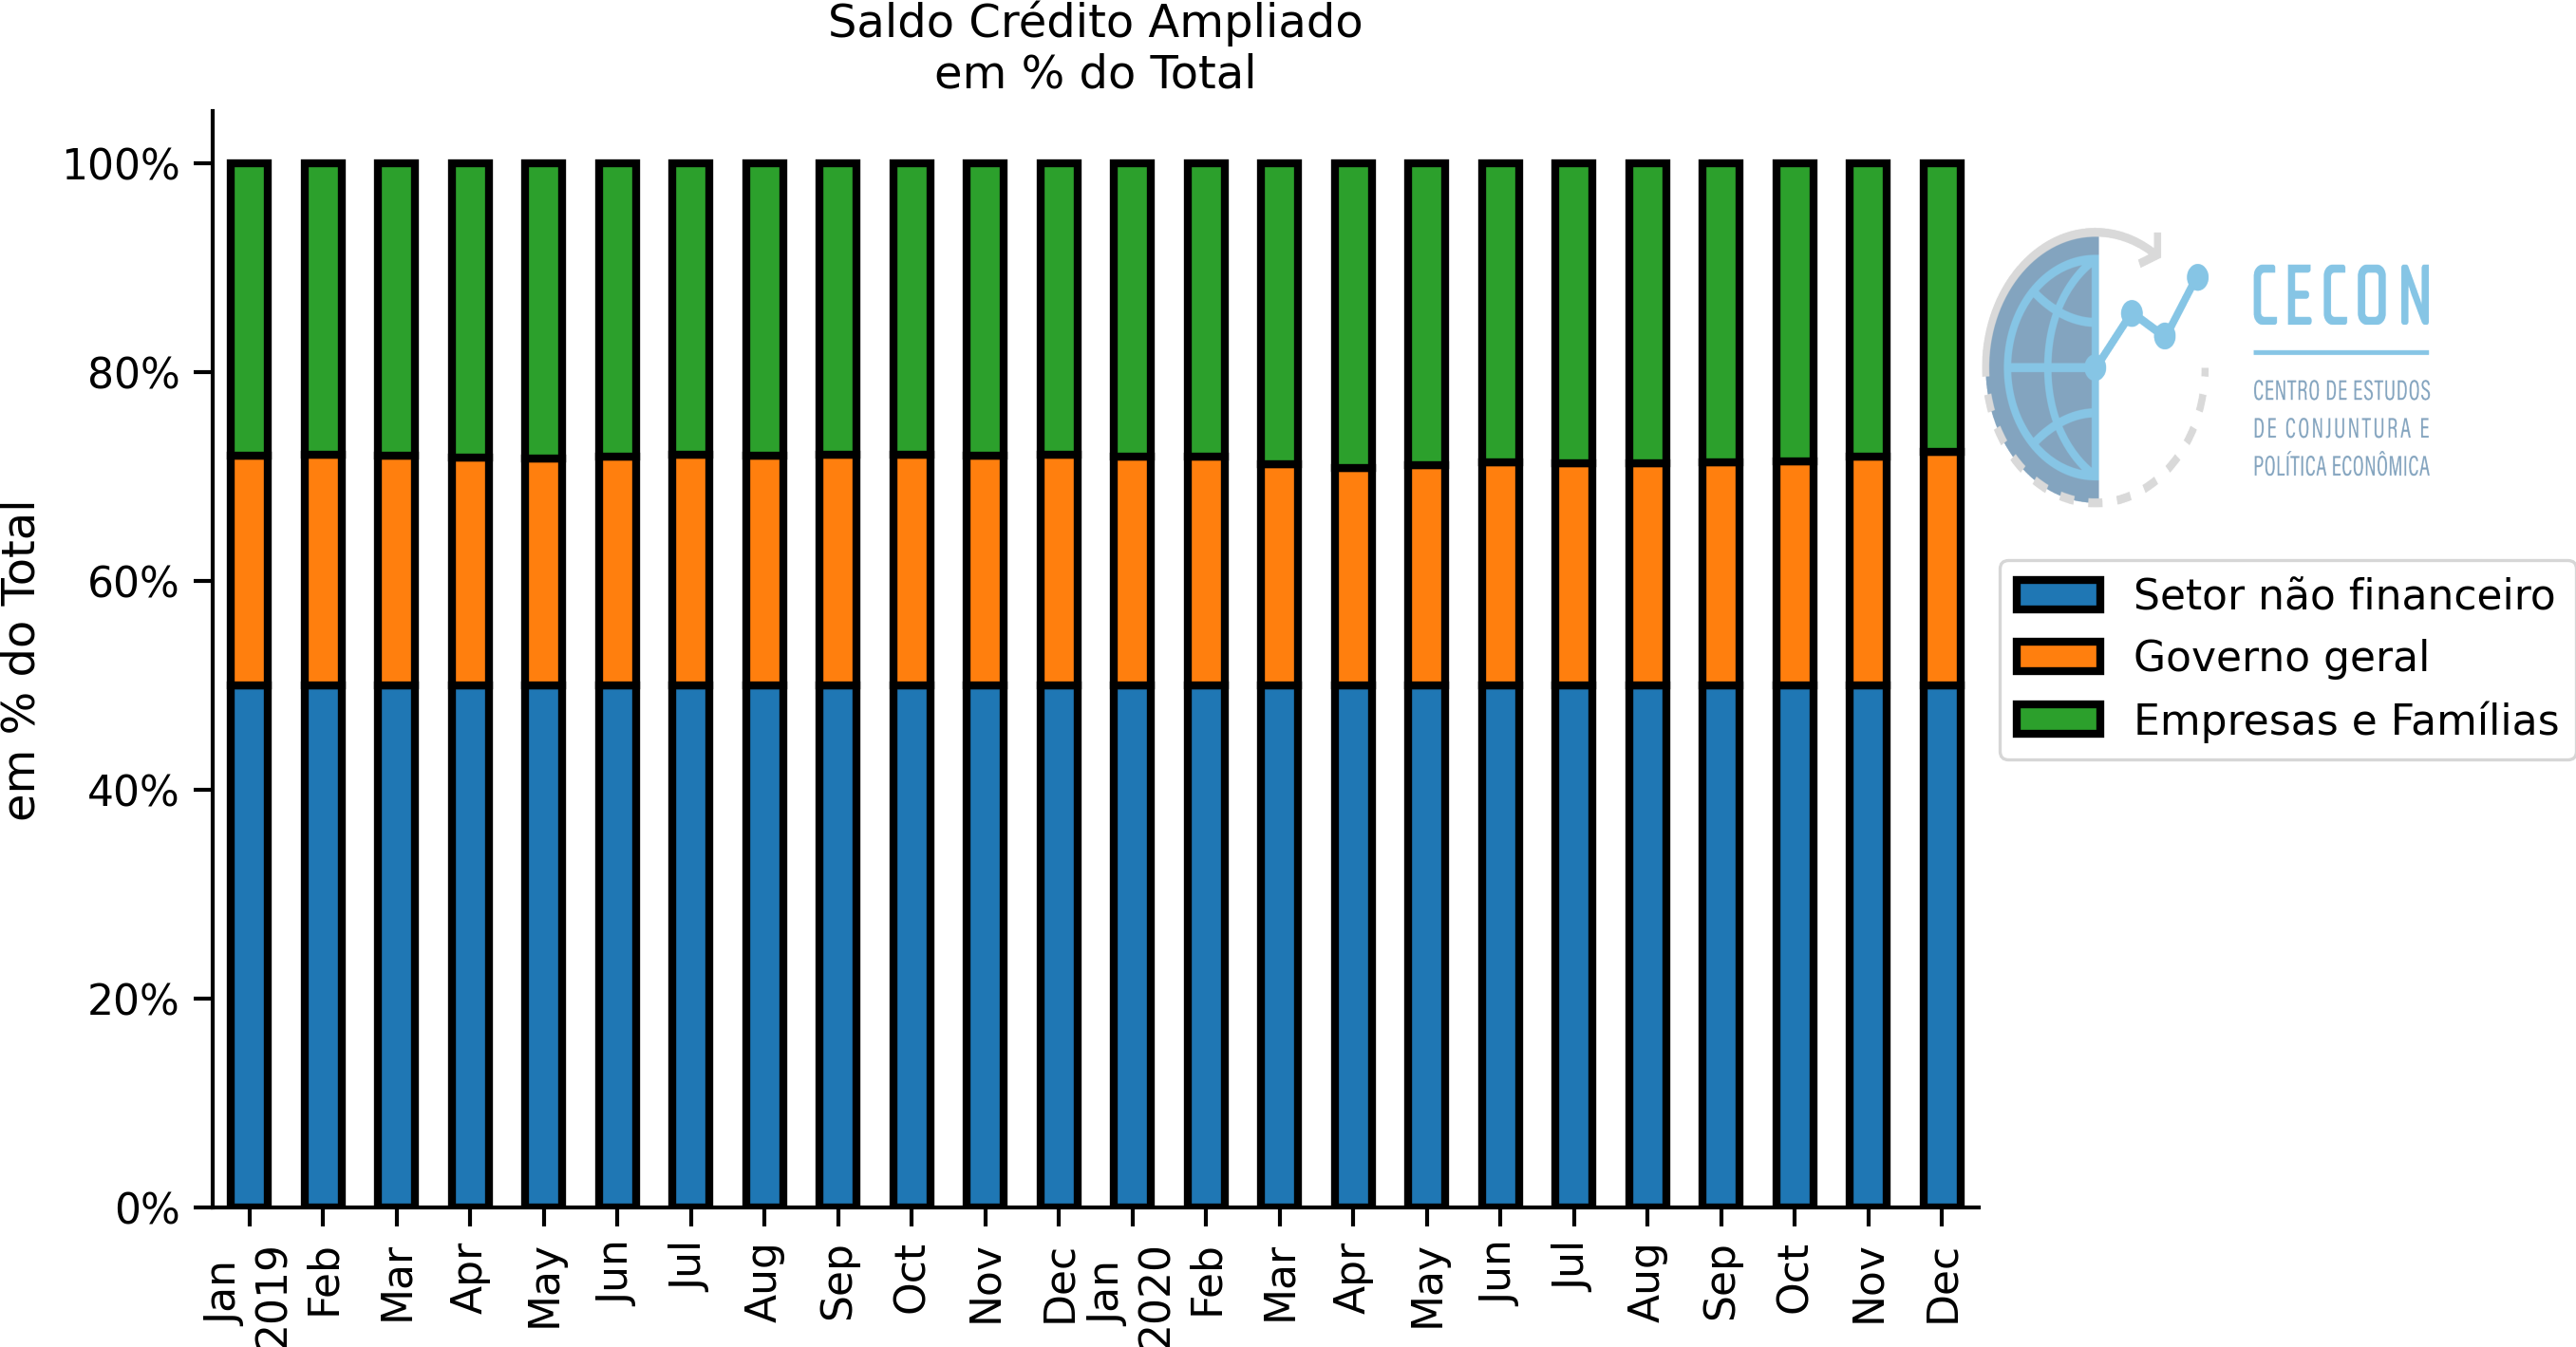
\includegraphics[width=.9\linewidth]{./figs/Credito/SaldoCreditoAmpliado_Total.png}
\end{center}

\subsection*{Indicadores de aprovação de crédito}
\label{sec:orgadcaa9b}

\begin{center}
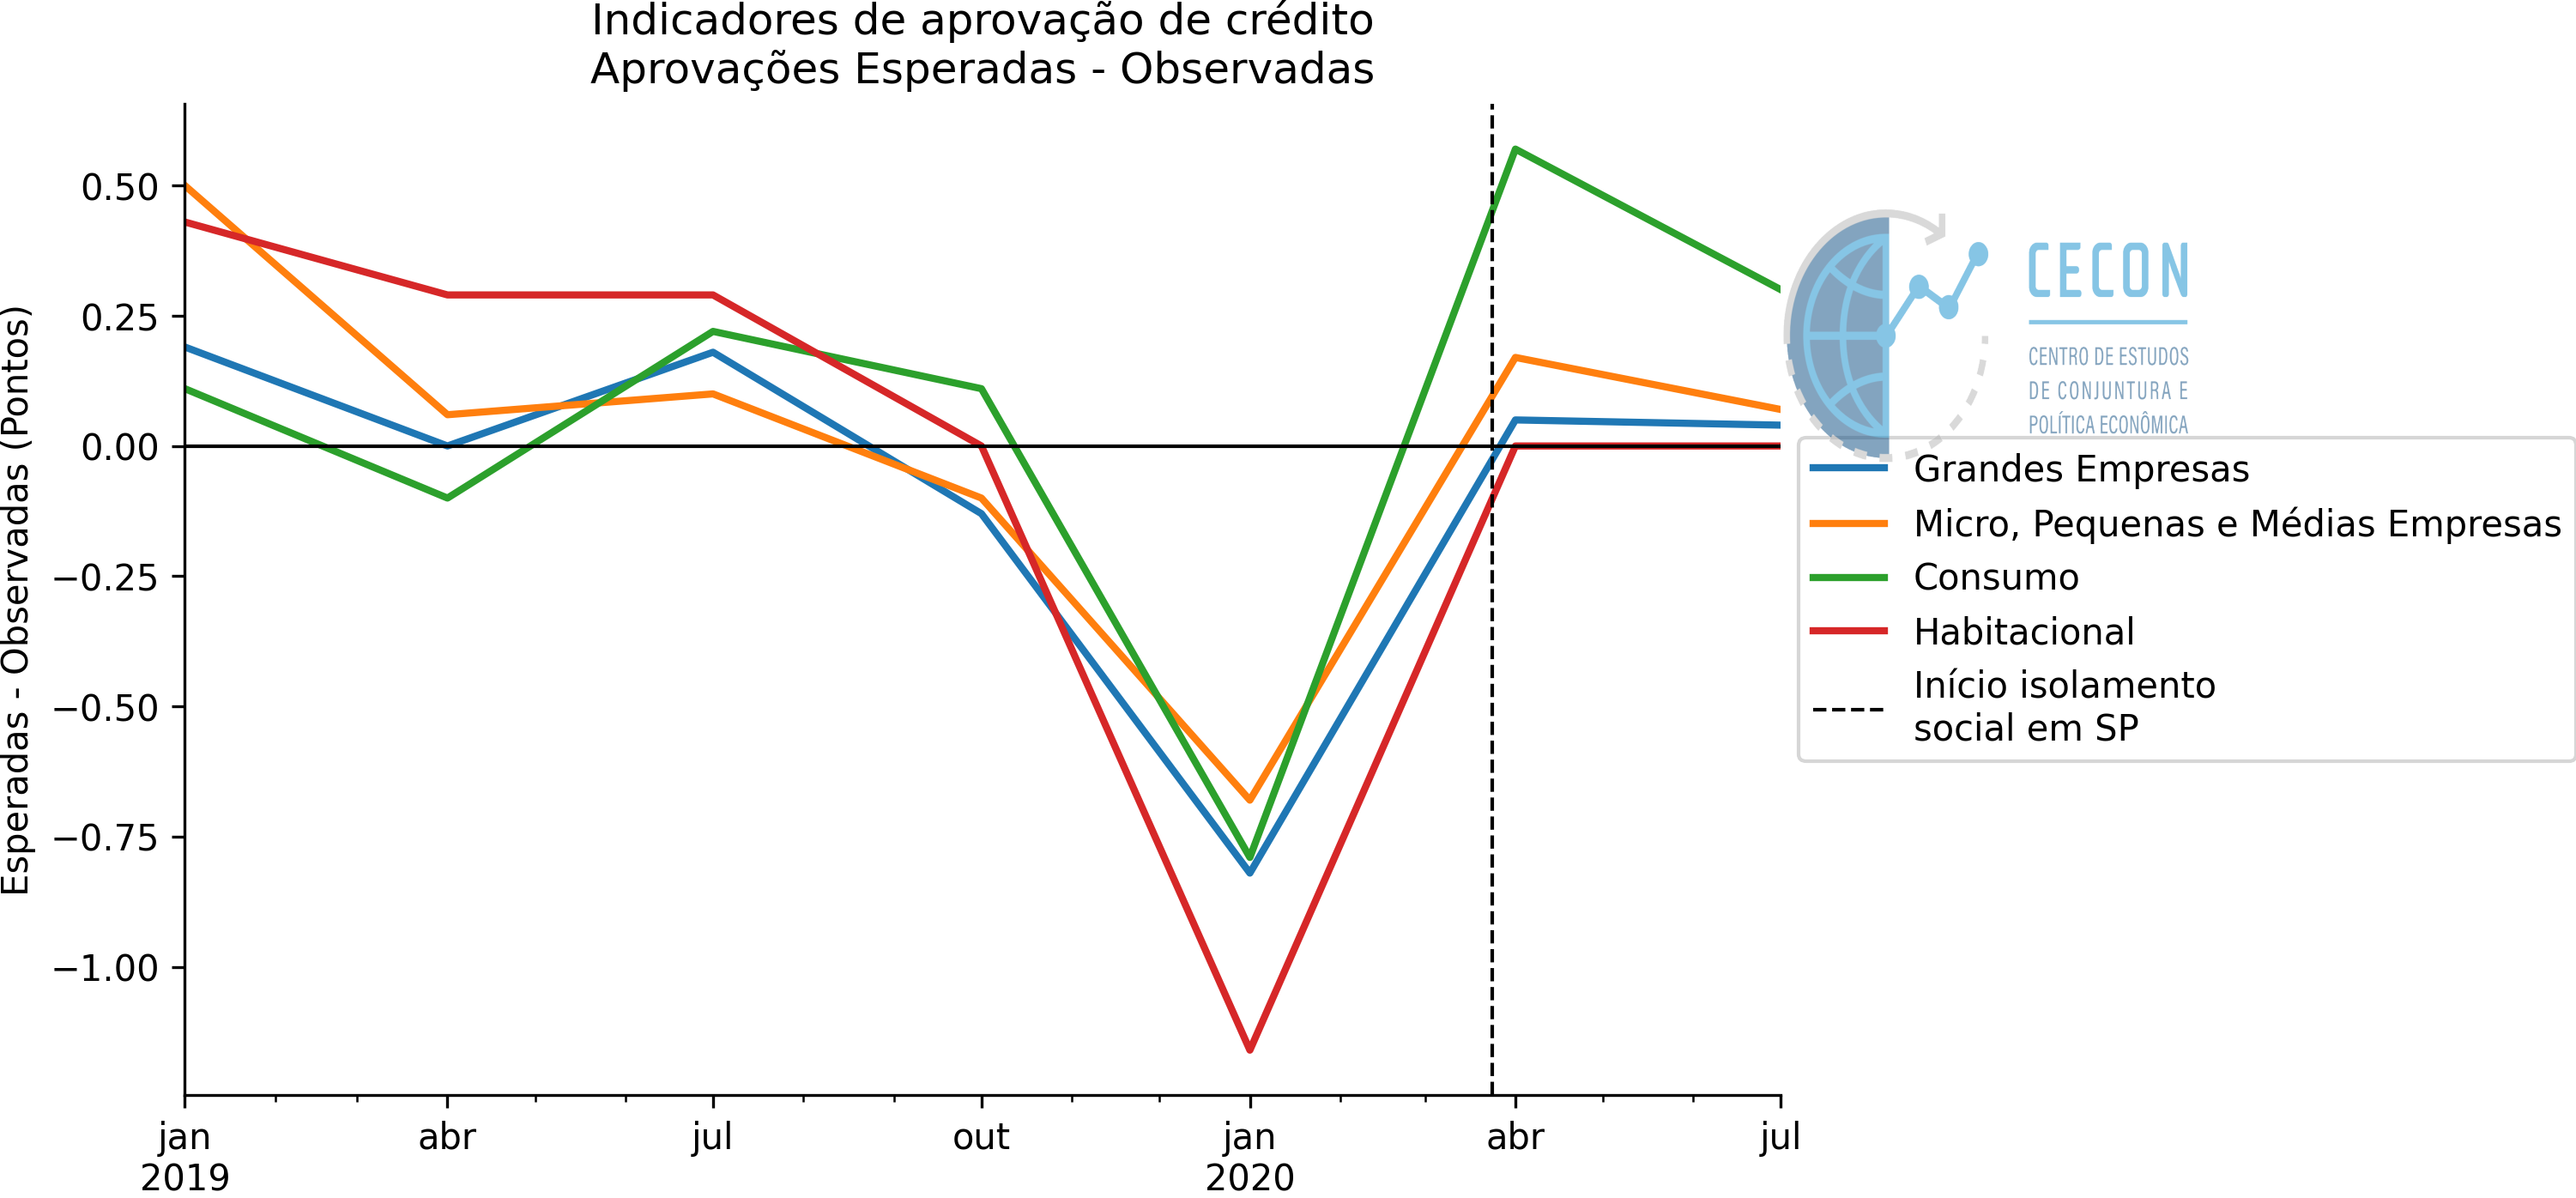
\includegraphics[width=.9\linewidth]{./figs/Credito/PTC.png}
\end{center}

\subsection*{Recolhimentos compulsórios de instituições financeiras}
\label{sec:org76fef48}

\begin{center}
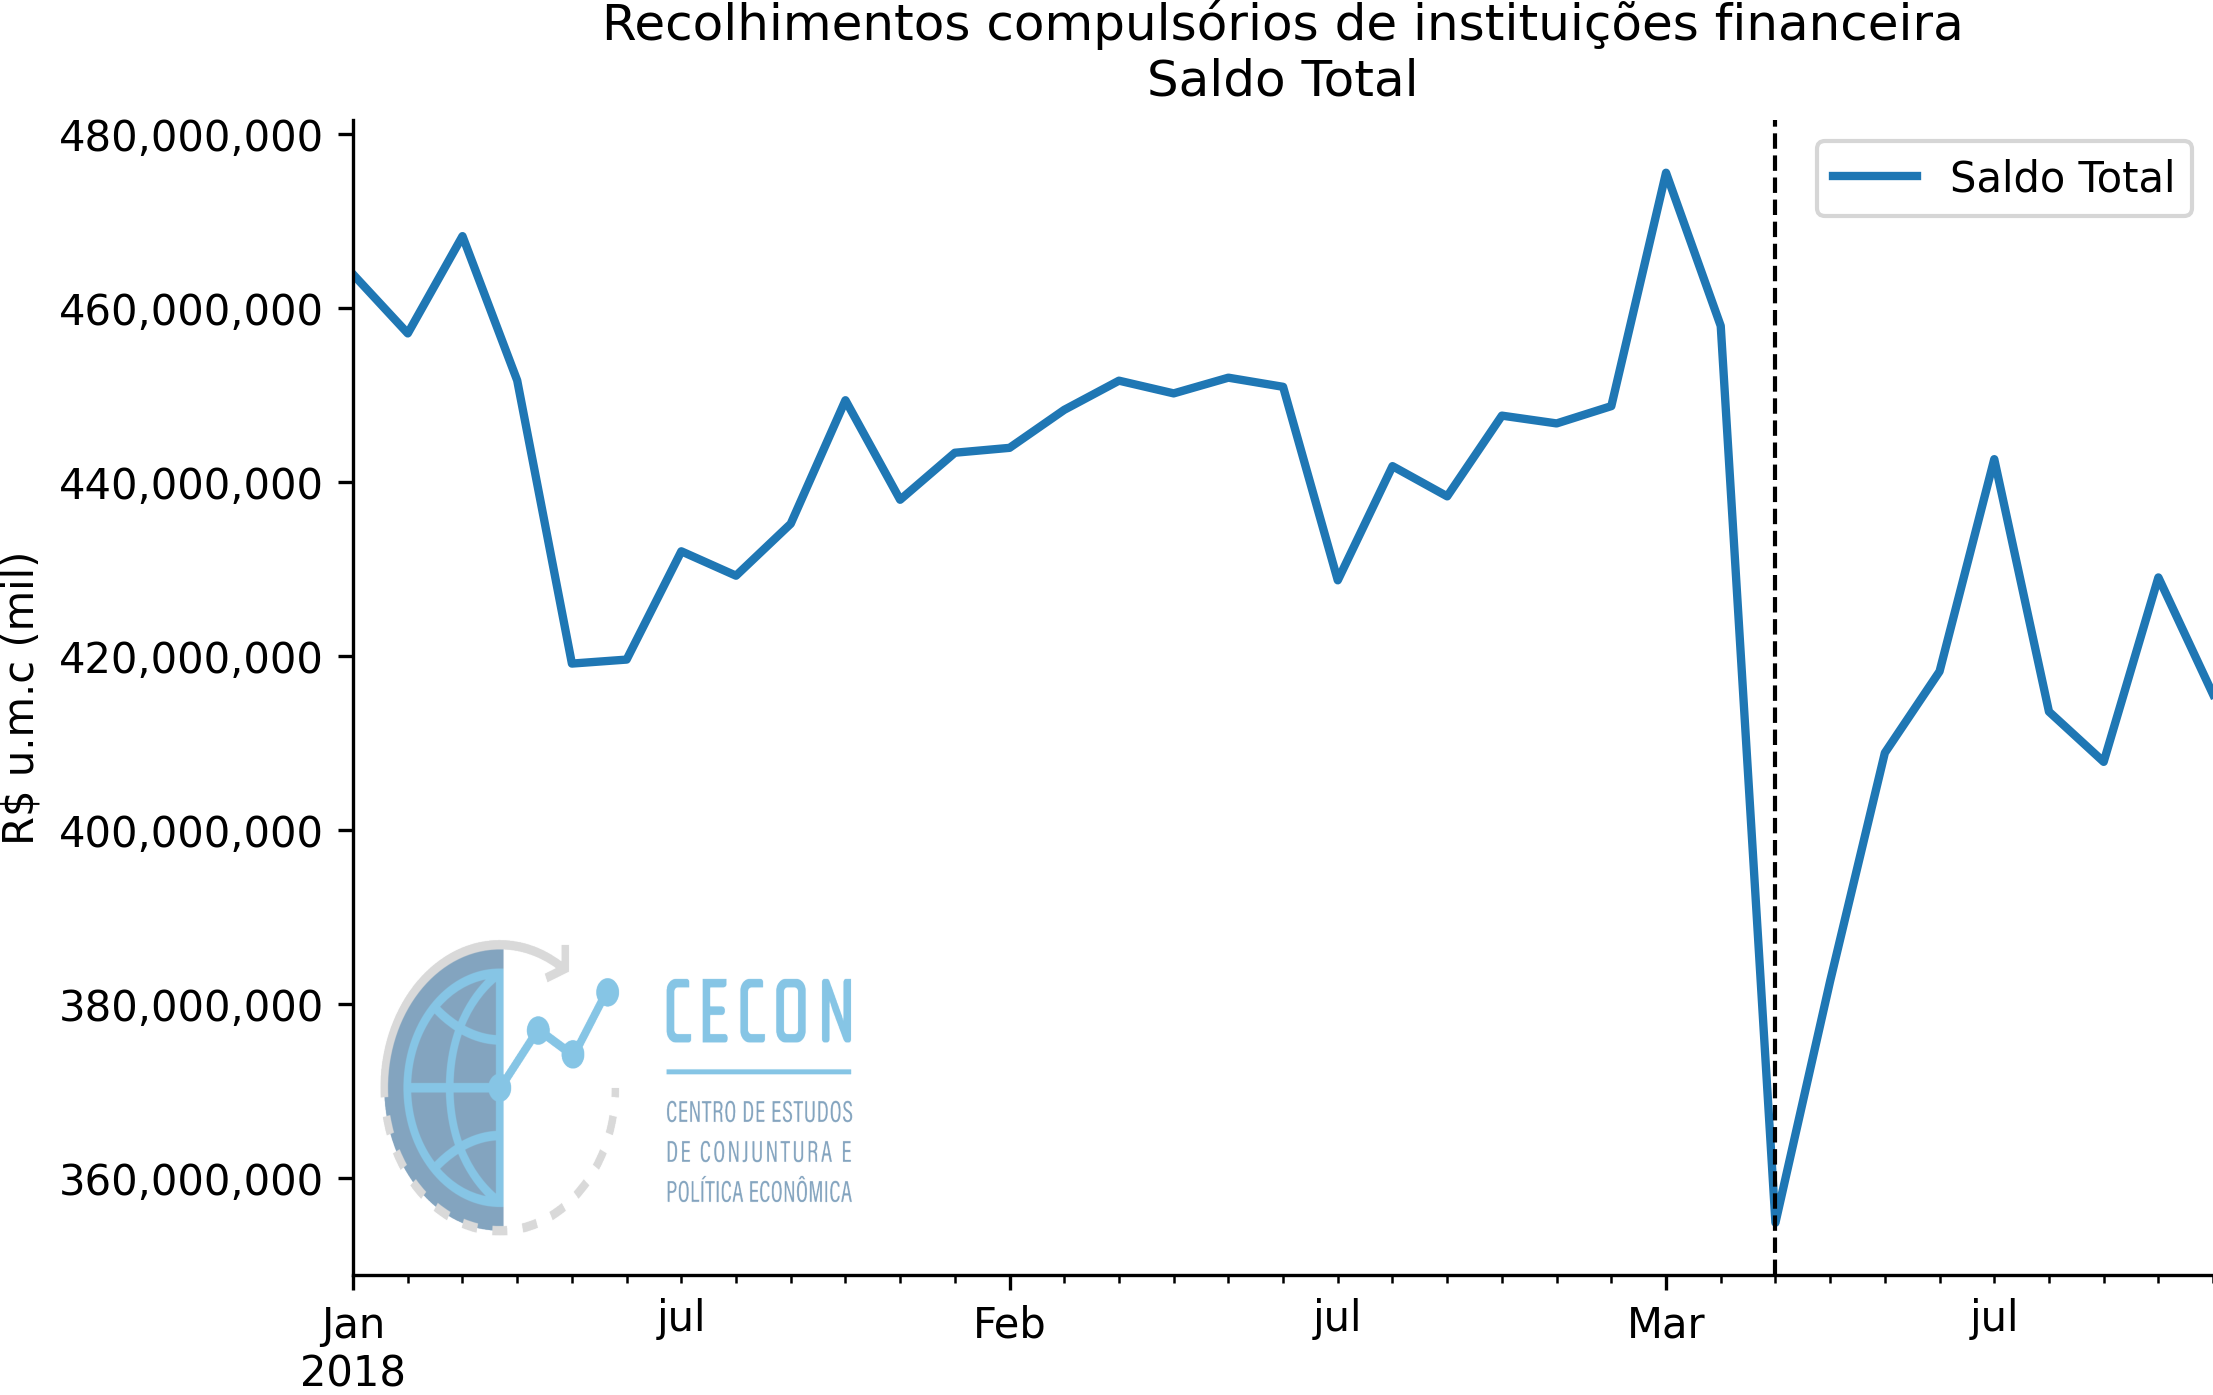
\includegraphics[width=.9\linewidth]{./figs/Credito/Recolhimentos_Total.png}
\end{center}

\section*{Índices de atividade setoriais}
\label{sec:orge1da2de}


\subsection*{Pesquisa Mensal do Comércio (PMC)}
\label{sec:orgede9753}

\begin{center}
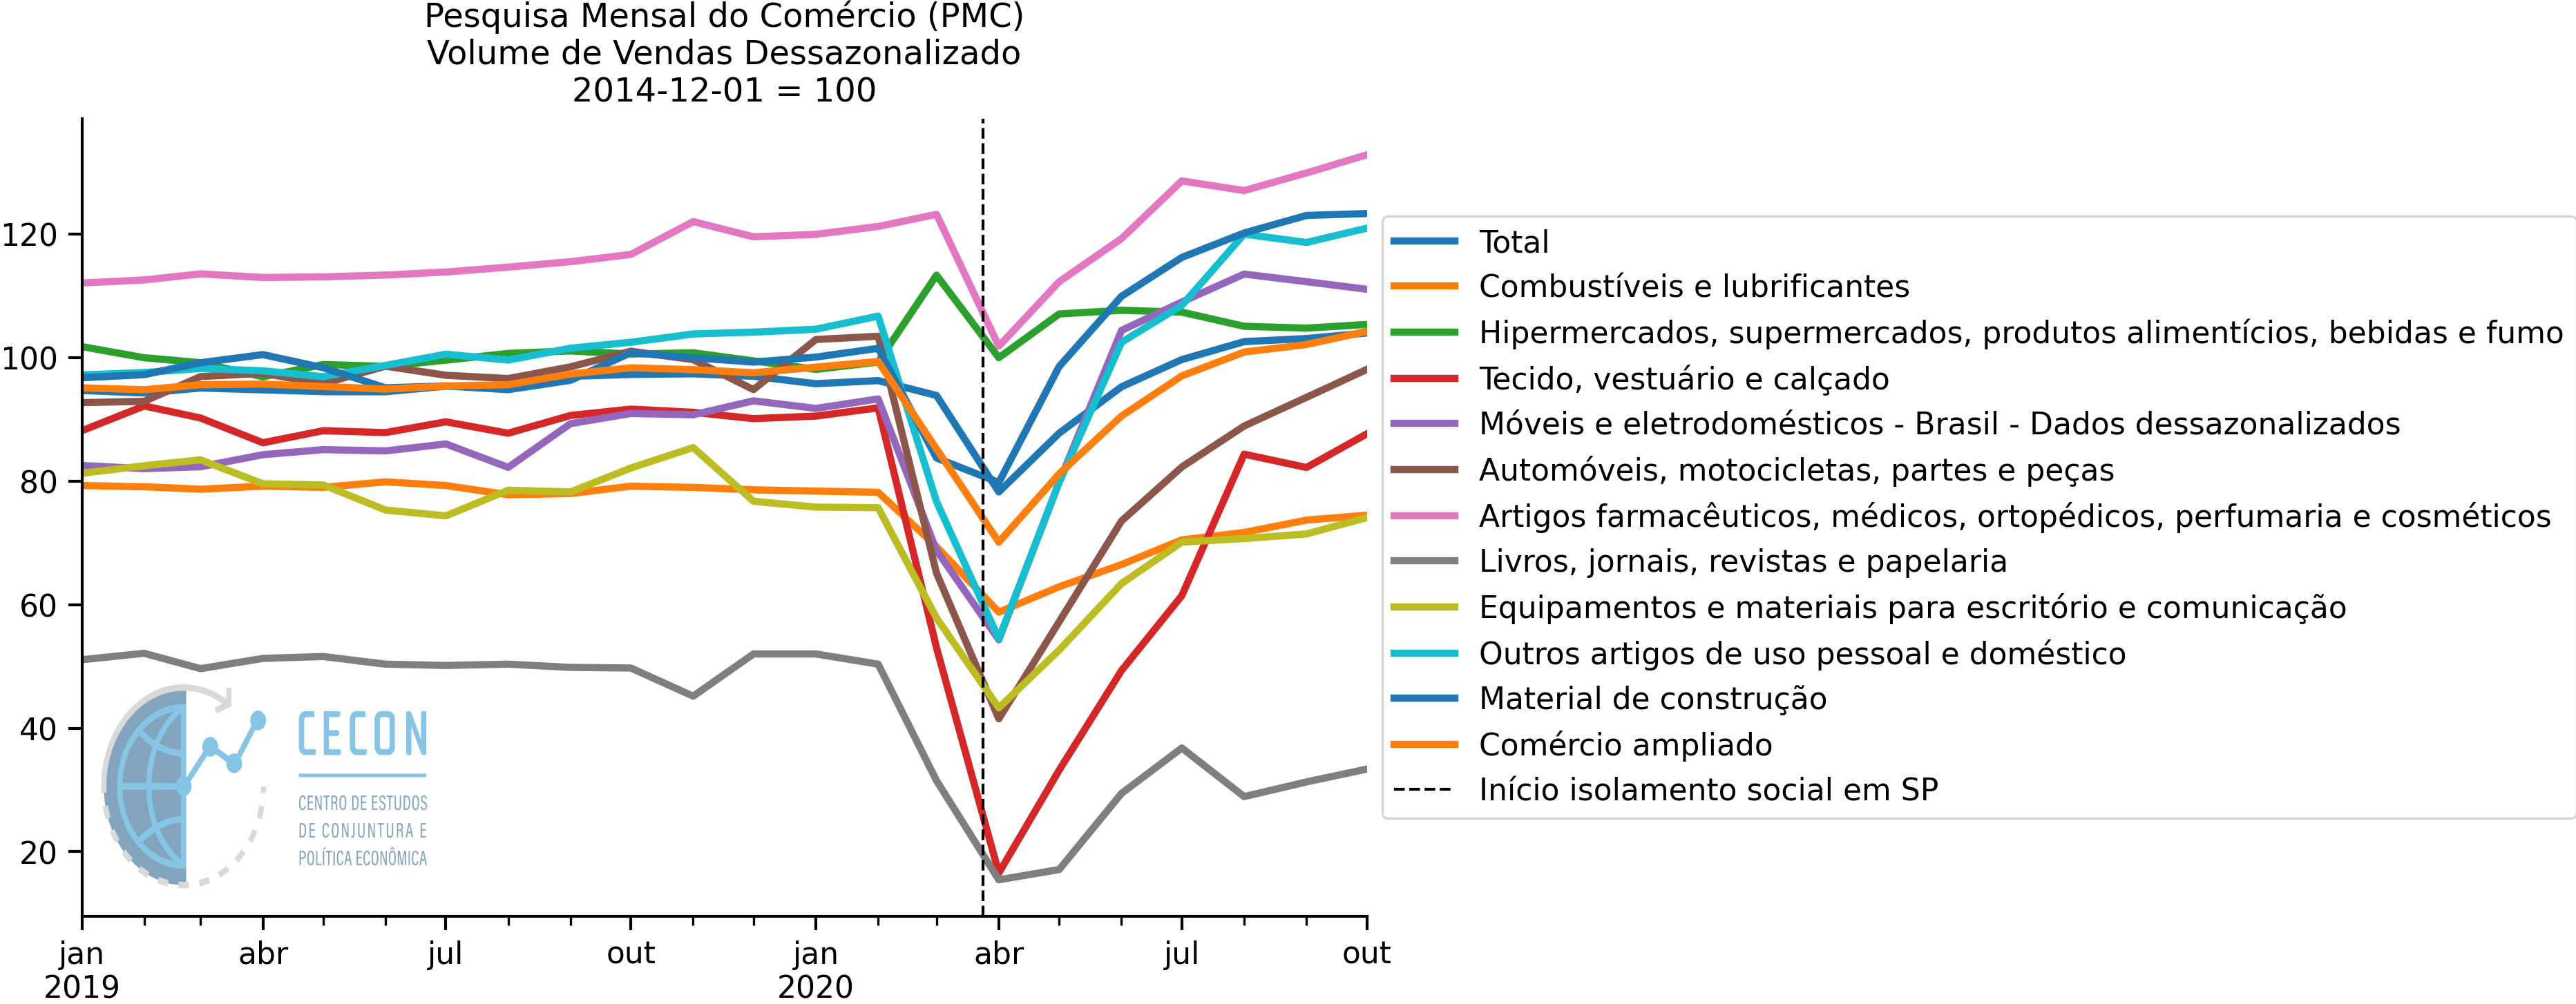
\includegraphics[width=.9\linewidth]{./figs/Setoriais/PMC_IBGE.png}
\end{center}


\subsection*{Pesquisa Industrial Mensal (PIM)}
\label{sec:orgd418176}

\begin{center}
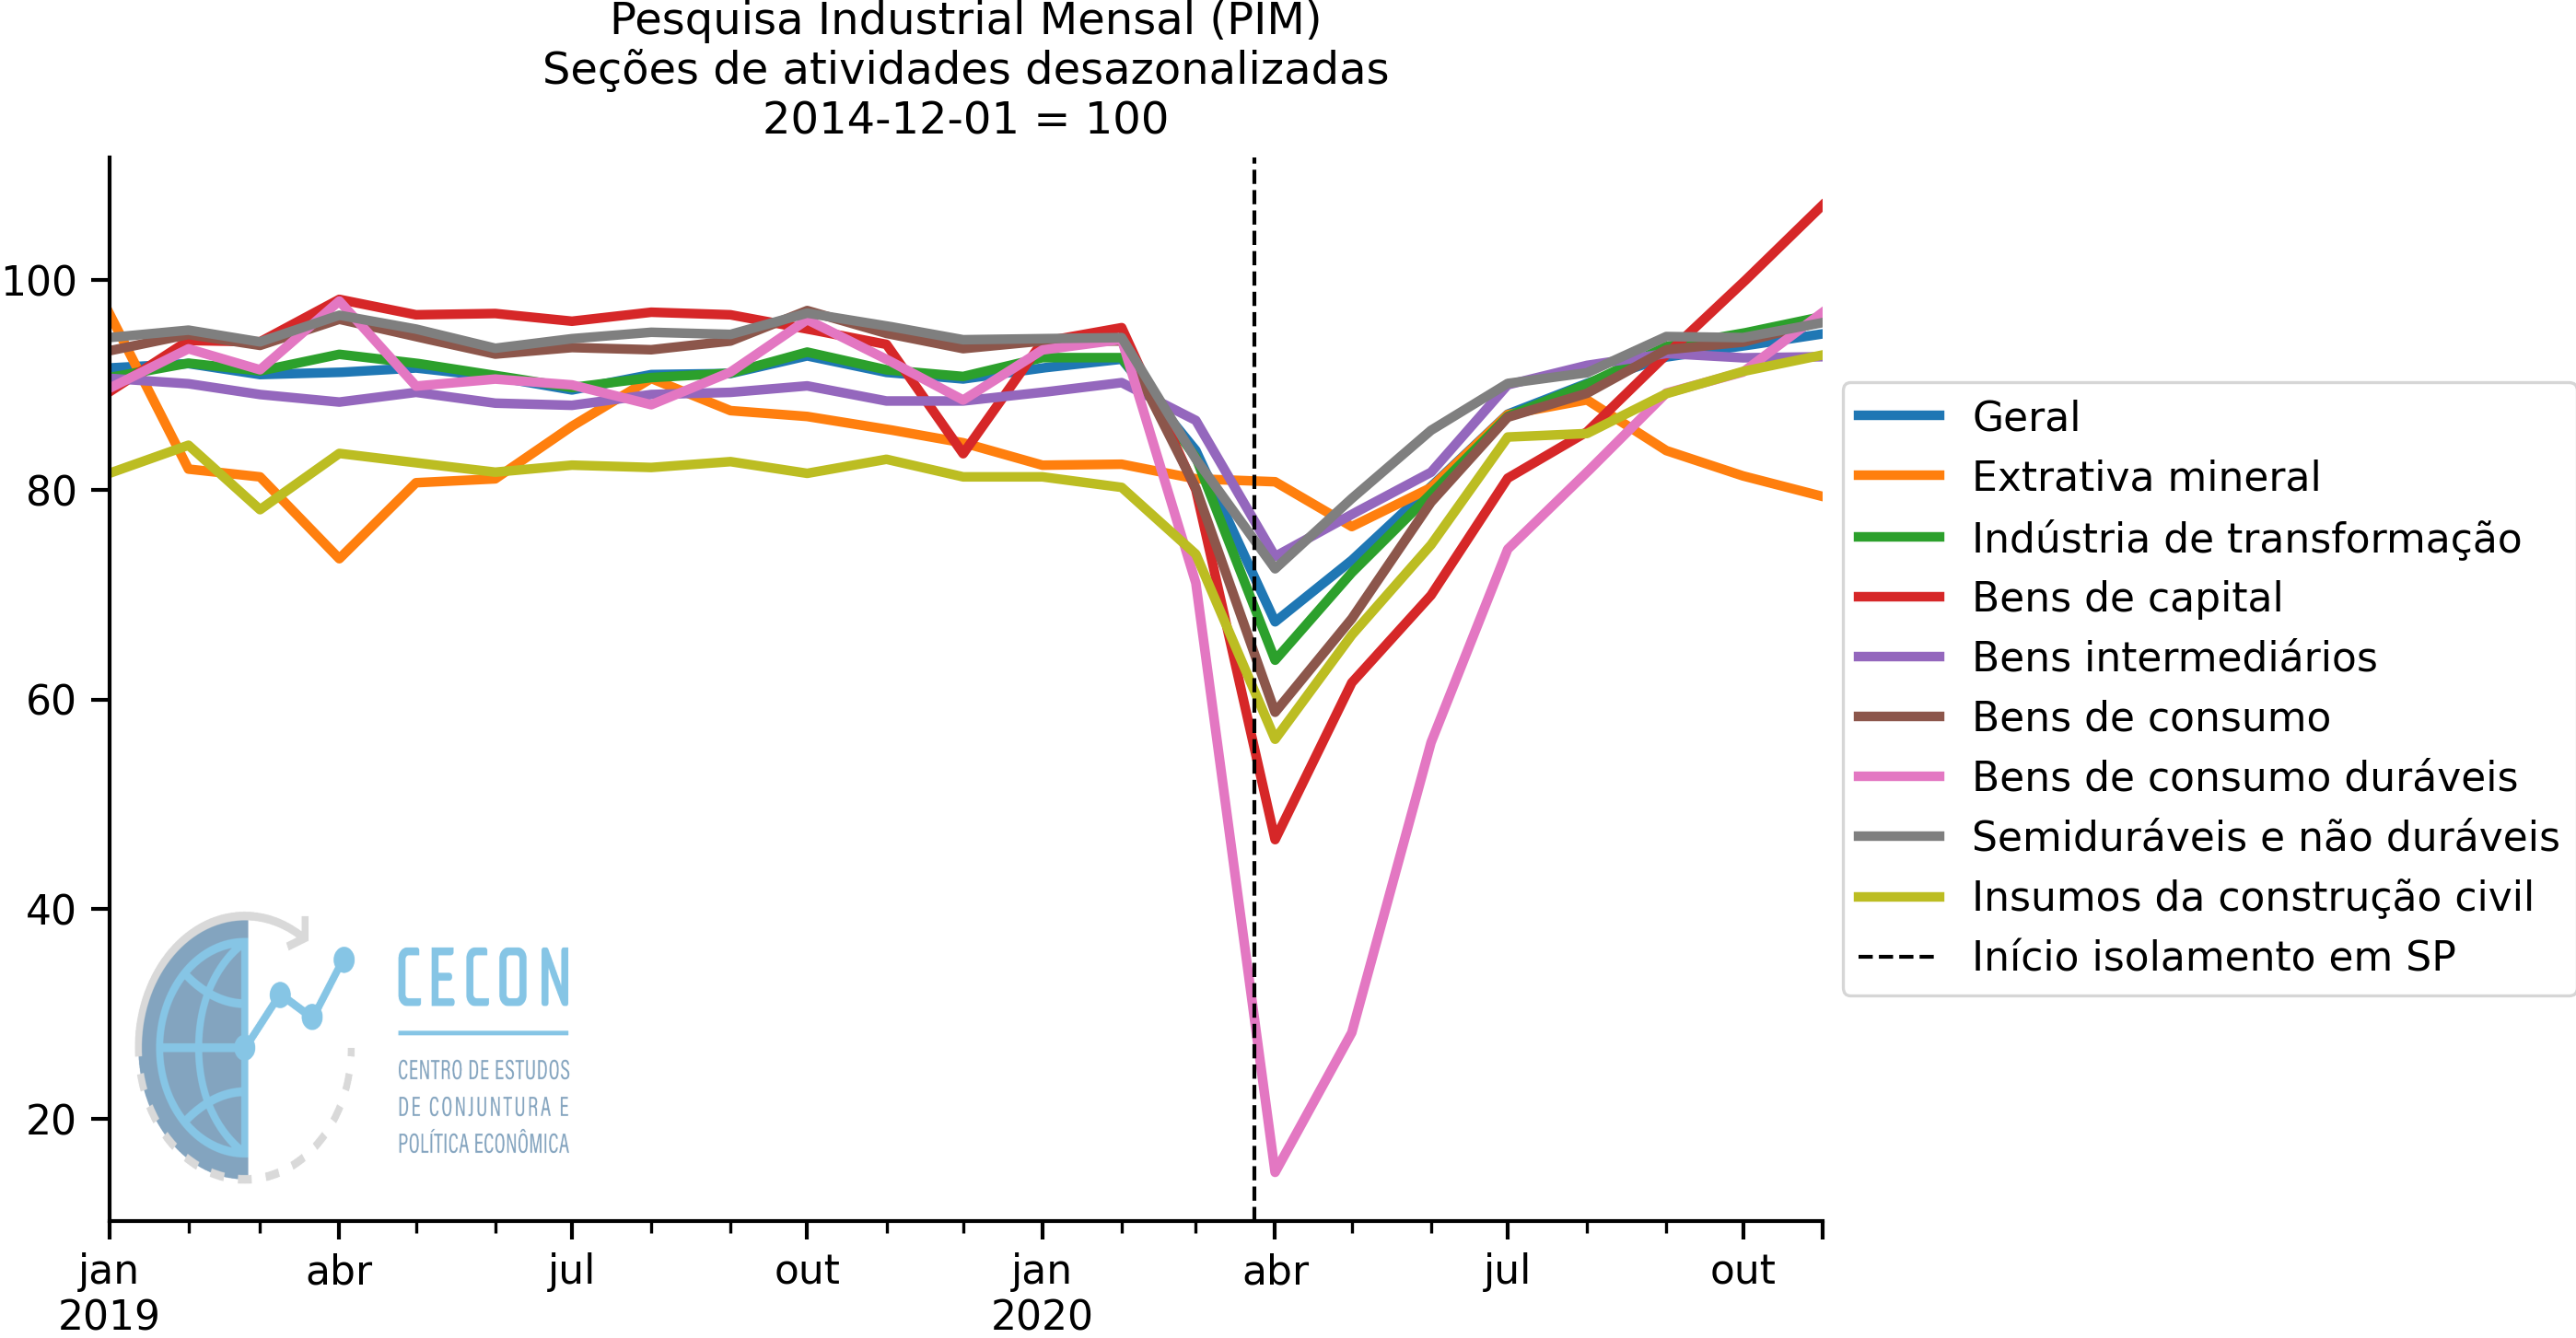
\includegraphics[width=.9\linewidth]{./figs/Setoriais/PIM_IBGE.png}
\end{center}


\subsection*{Pesquisa Mensal de Serviços (PMS)}
\label{sec:org92c7ff2}

\begin{center}
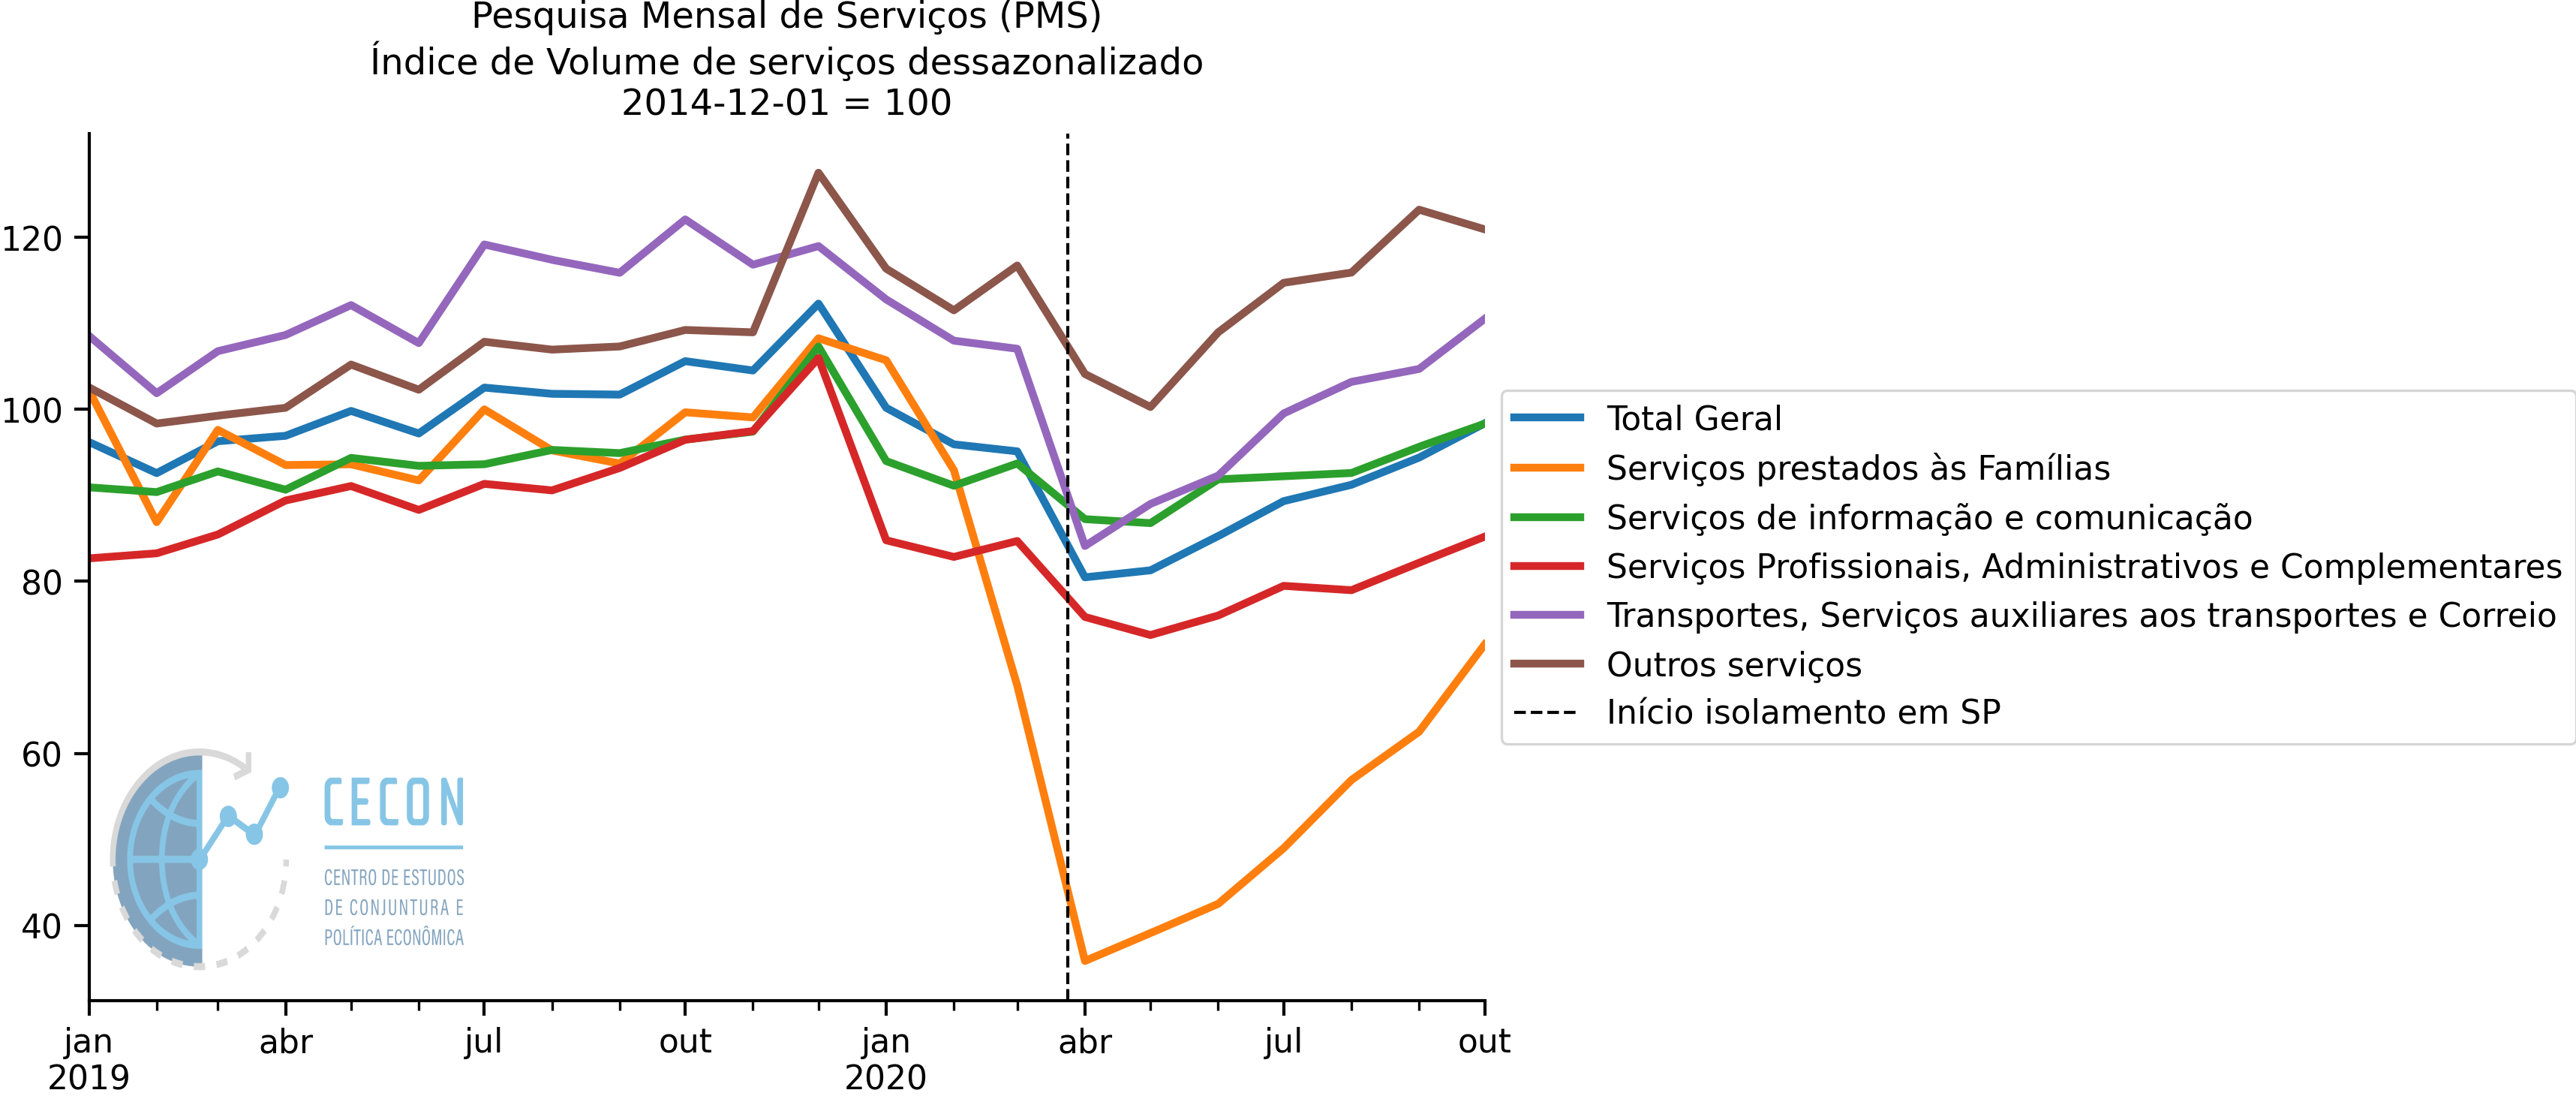
\includegraphics[width=.9\linewidth]{./figs/Setoriais/PMS_IBGE.png}
\end{center}

\section*{Emprego}
\label{sec:org319ed7c}

\subsection*{Rendimento médio real habitual das pessoas ocupadas}
\label{sec:org70640b1}


\begin{center}
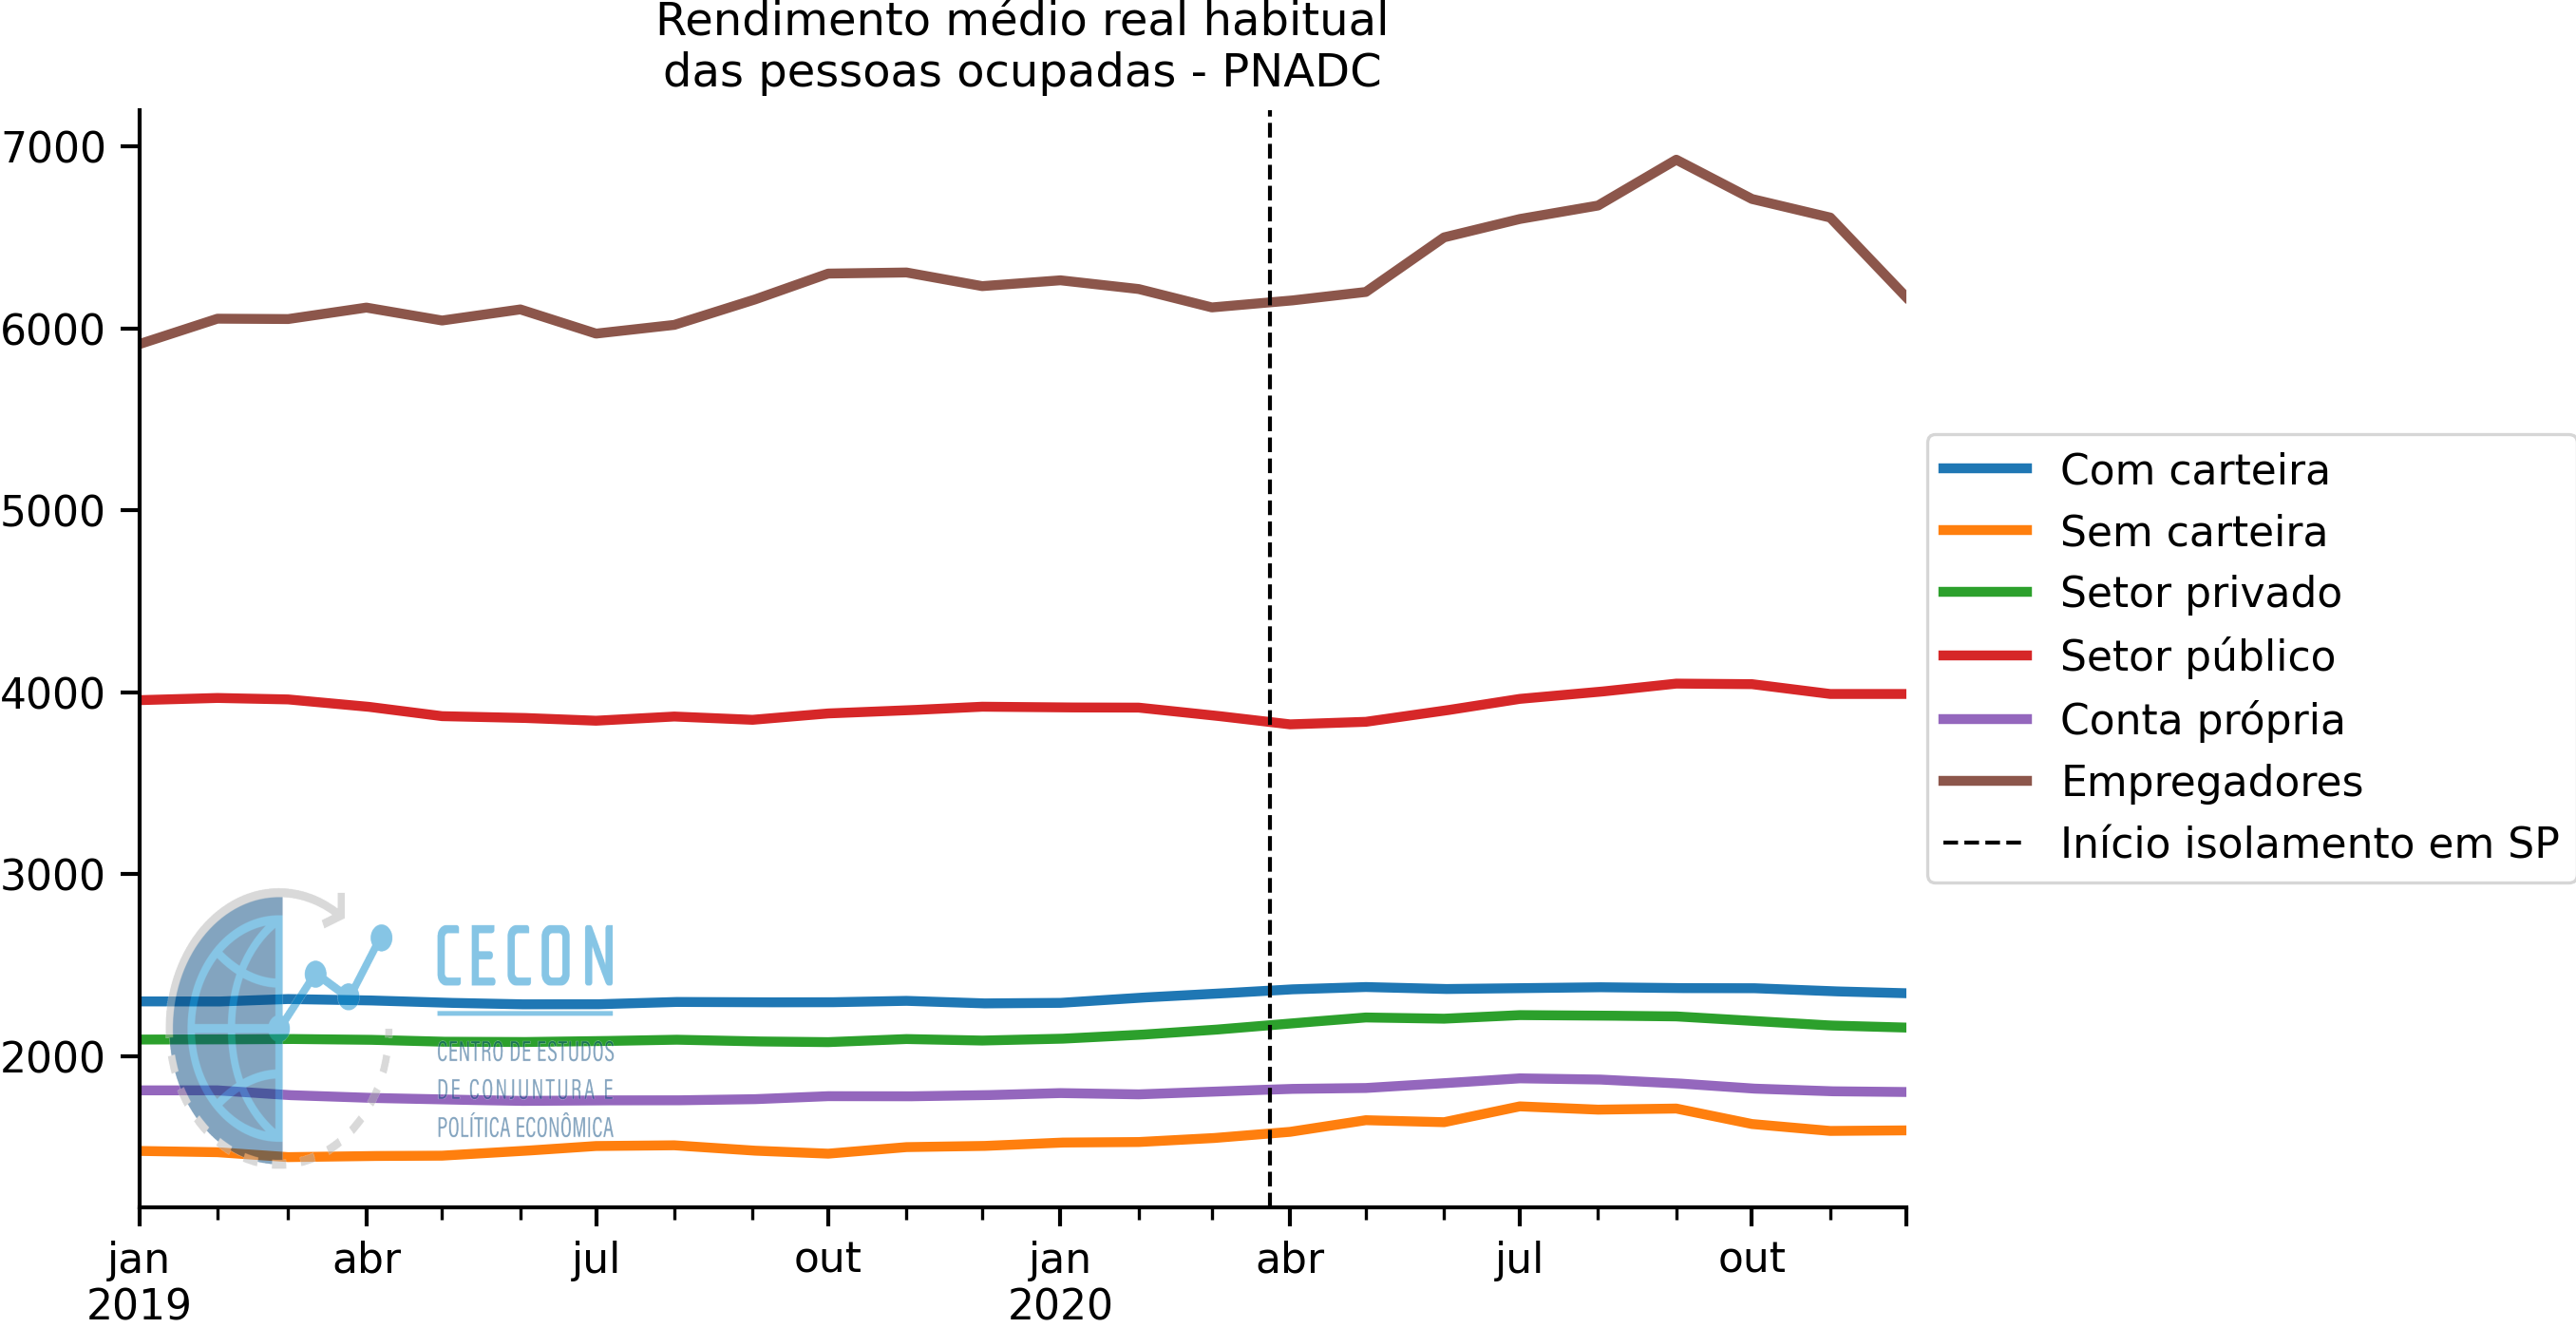
\includegraphics[width=.9\linewidth]{./figs/Emprego/RMHPO.png}
\end{center}

\subsection*{Massa de rendimento real efetiva e habitual de todos os trabalhos}
\label{sec:org801741c}

\begin{center}
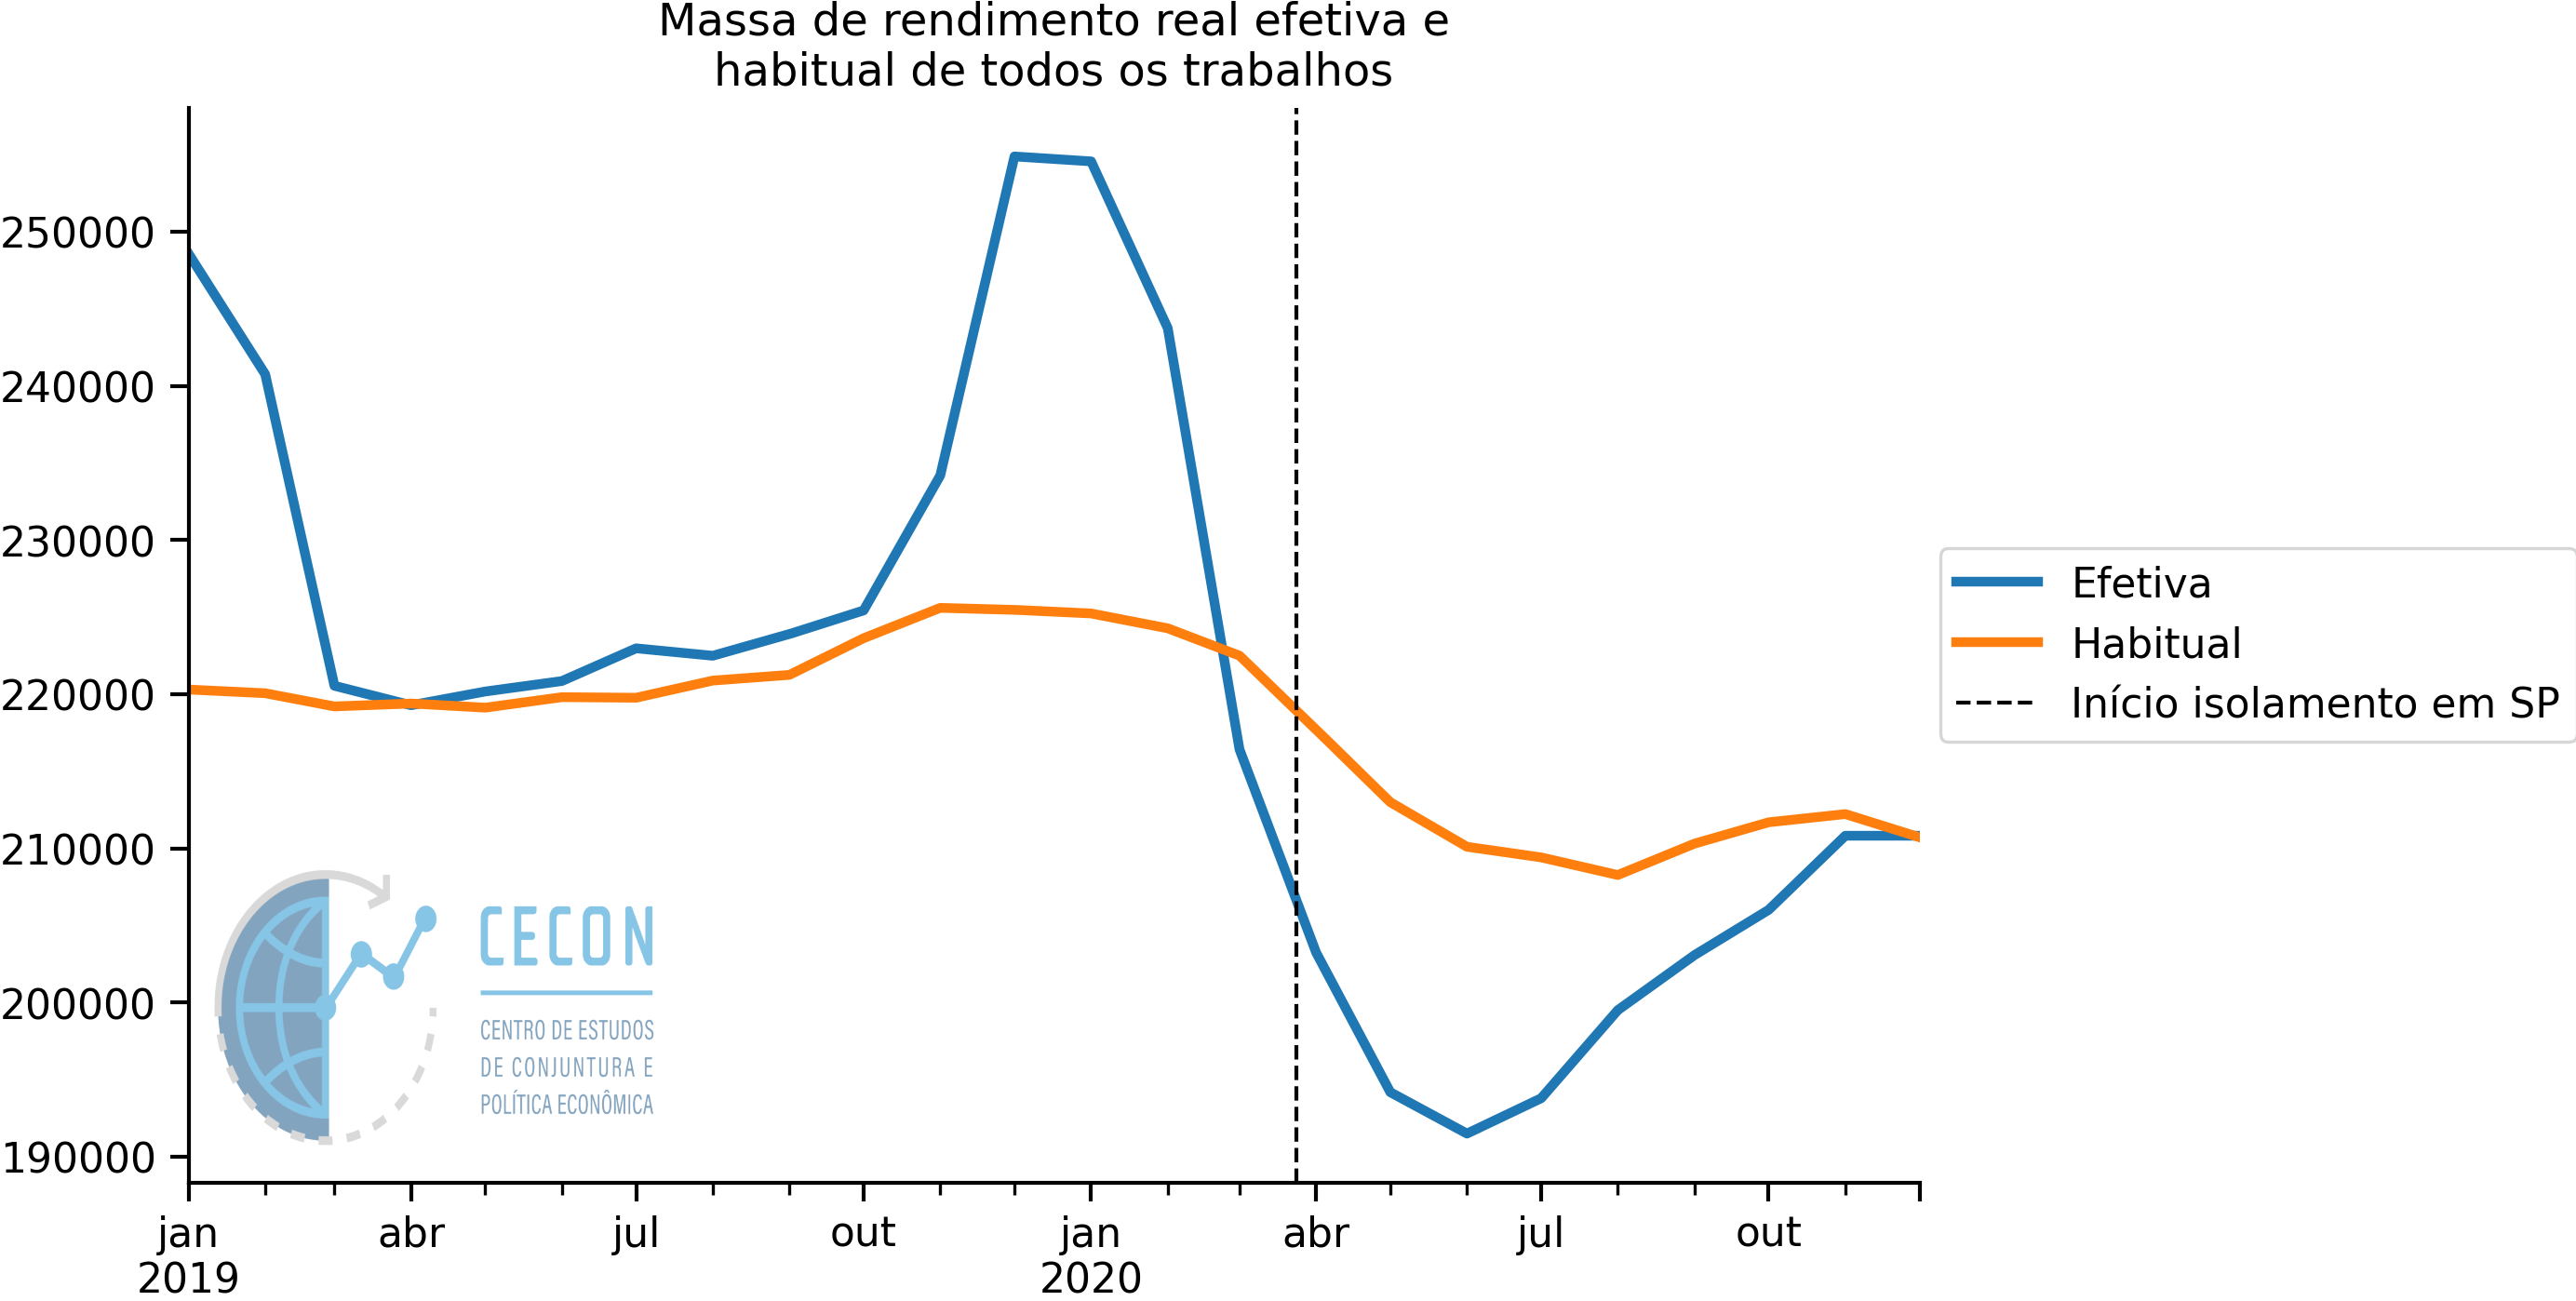
\includegraphics[width=.9\linewidth]{./figs/Emprego/MRR_Efetiva_Habitual.png}
\end{center}

\subsection*{Massa Salarial Ampliada Disponível - PNADC}
\label{sec:org38c527c}

\begin{center}
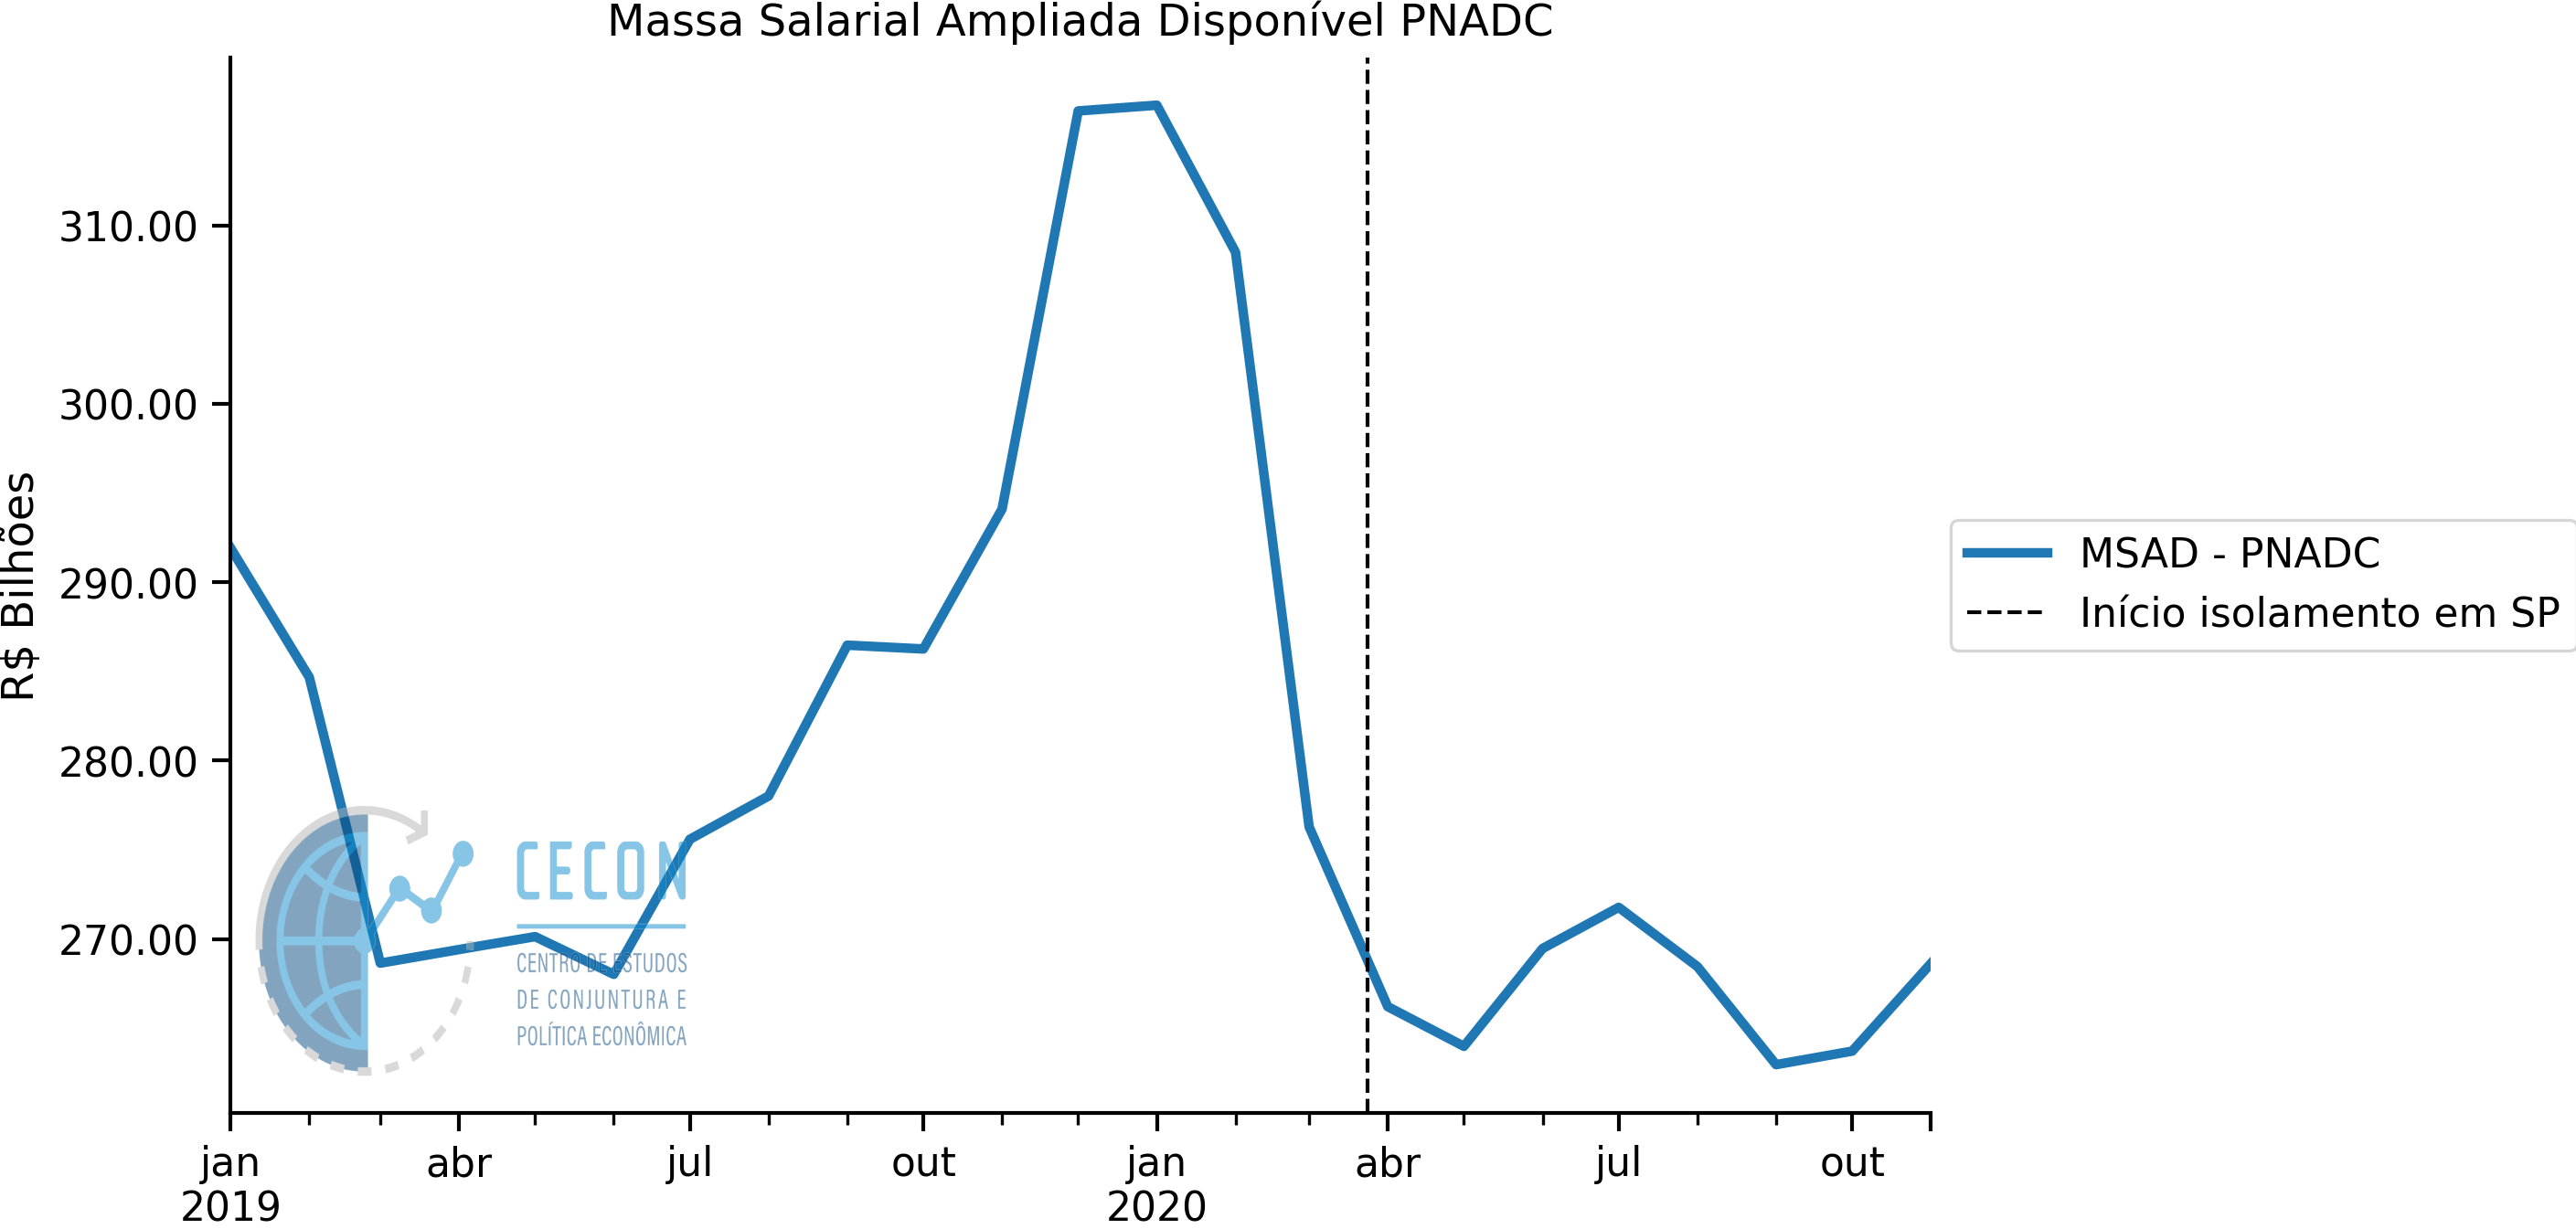
\includegraphics[width=.9\linewidth]{./figs/Emprego/MSAD.png}
\end{center}

\subsection*{Rendimento habitual médio por atividade}
\label{sec:orgc31d960}

\subsection*{Número de horas trabalhadas - indústria de transformação}
\label{sec:org1fa353f}

\begin{center}
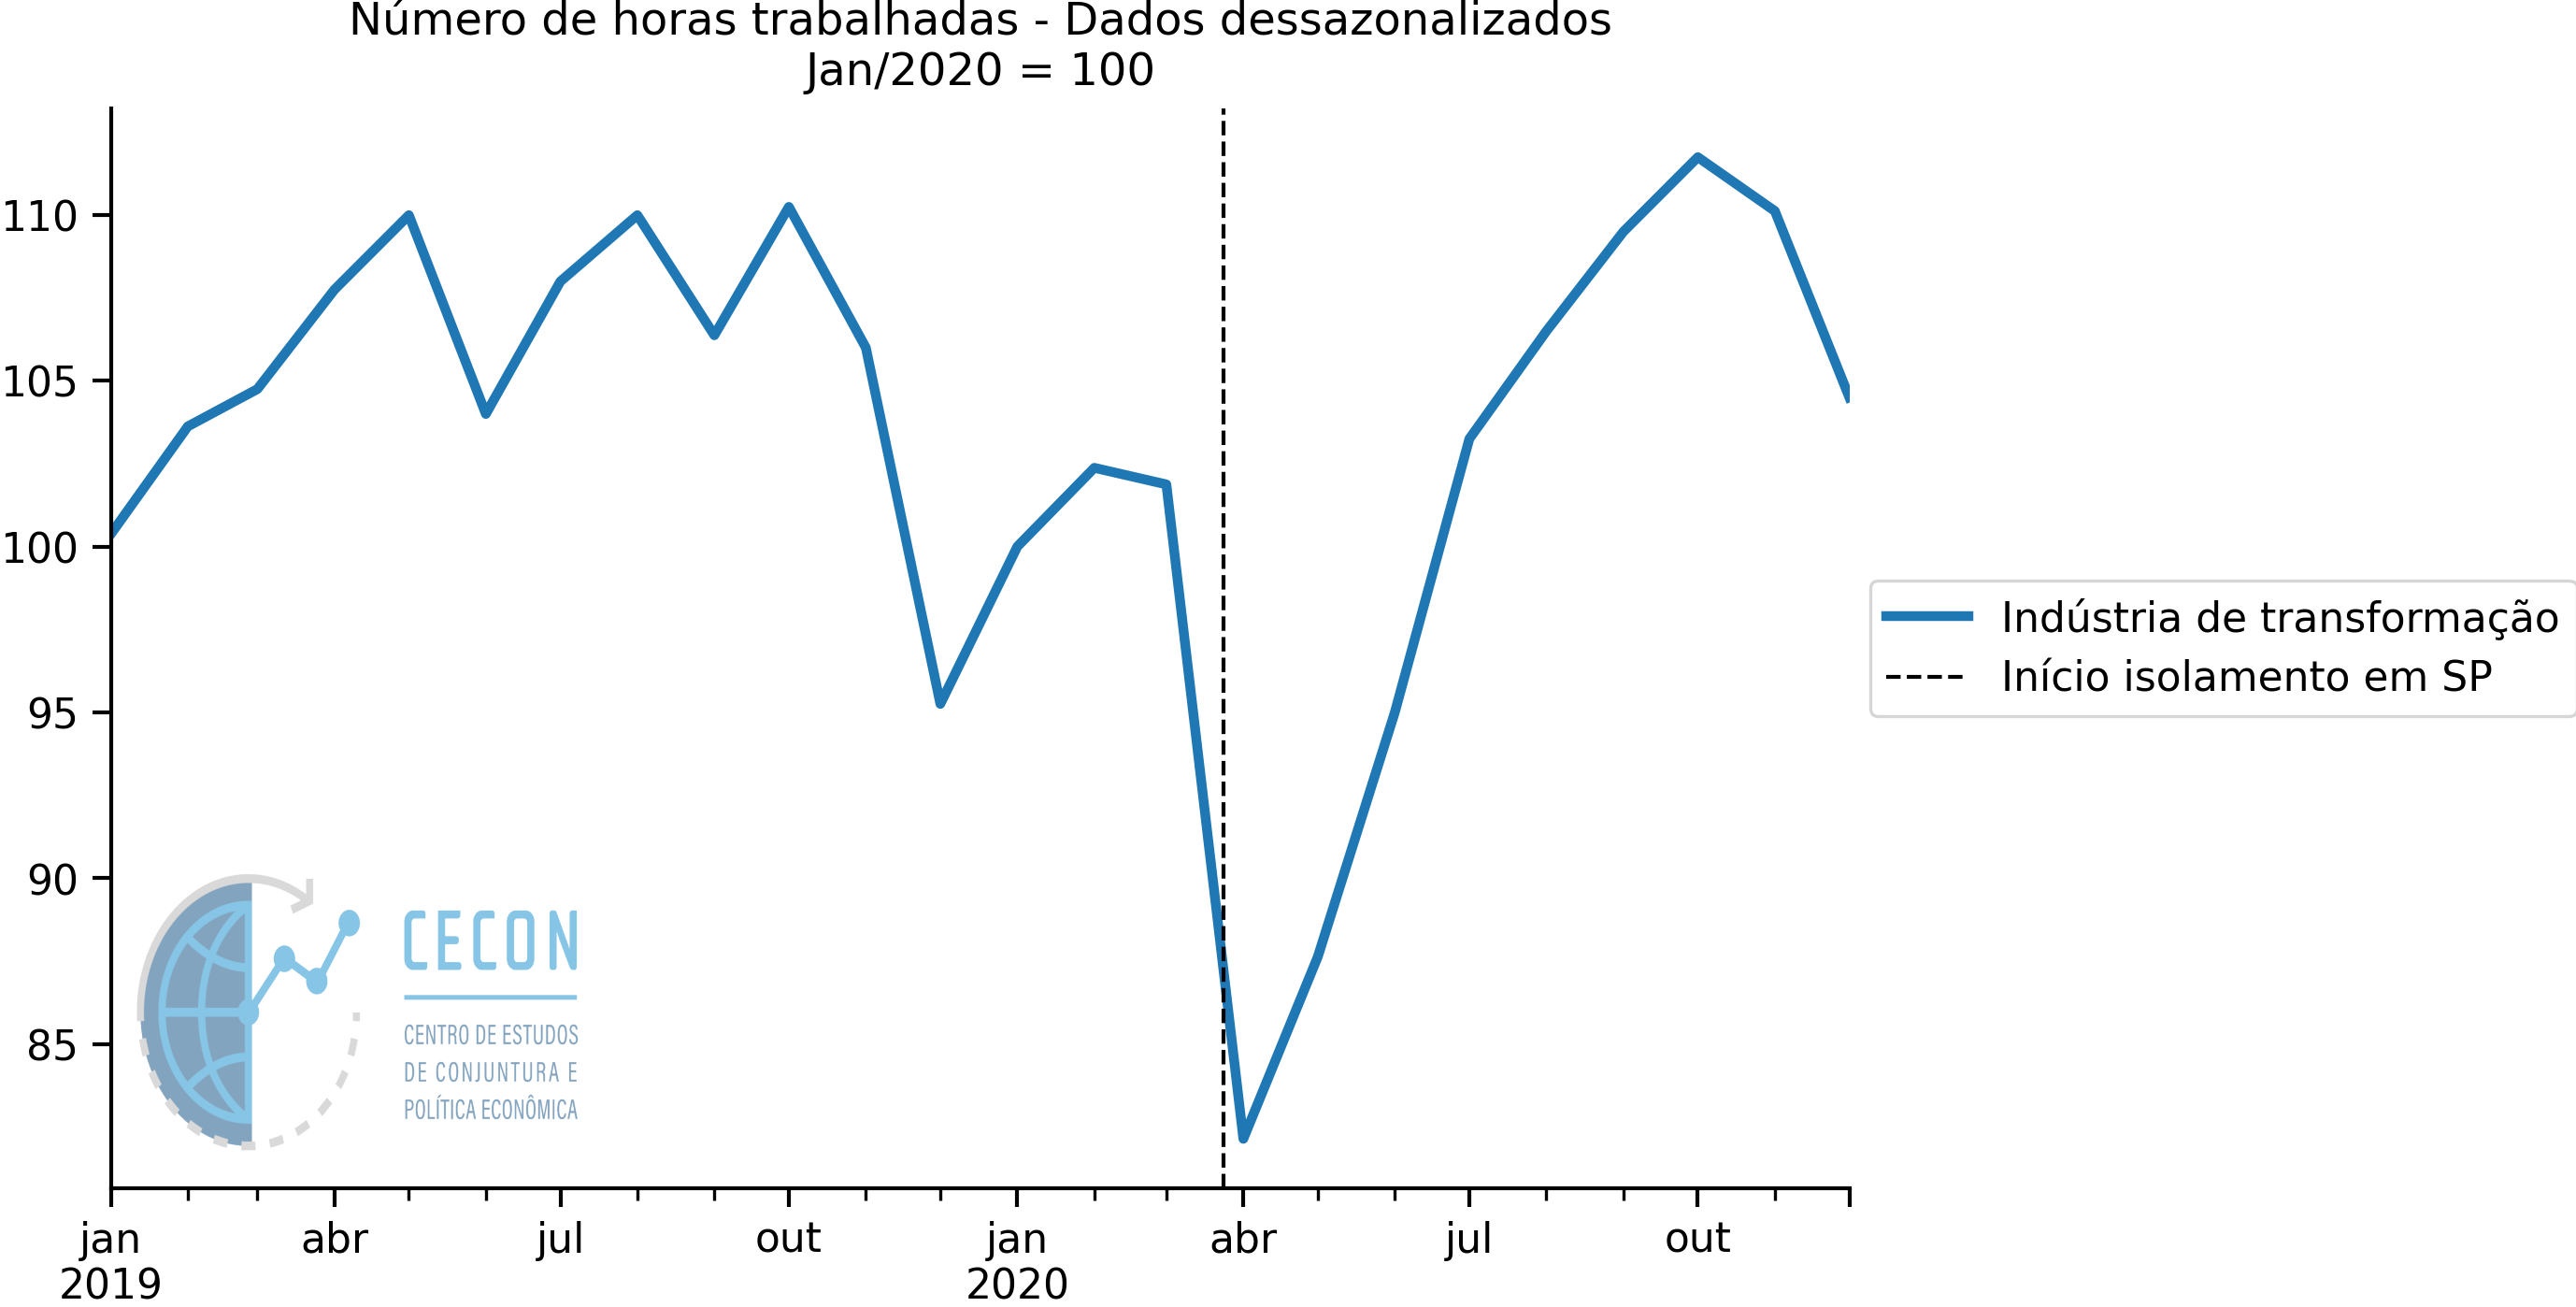
\includegraphics[width=.9\linewidth]{./figs/Emprego/Horas_Transformacao.png}
\end{center}

\subsection*{Novo CAGED  - Por atividade (dados dessazonalizados)}
\label{sec:org2b38c4d}

\begin{center}
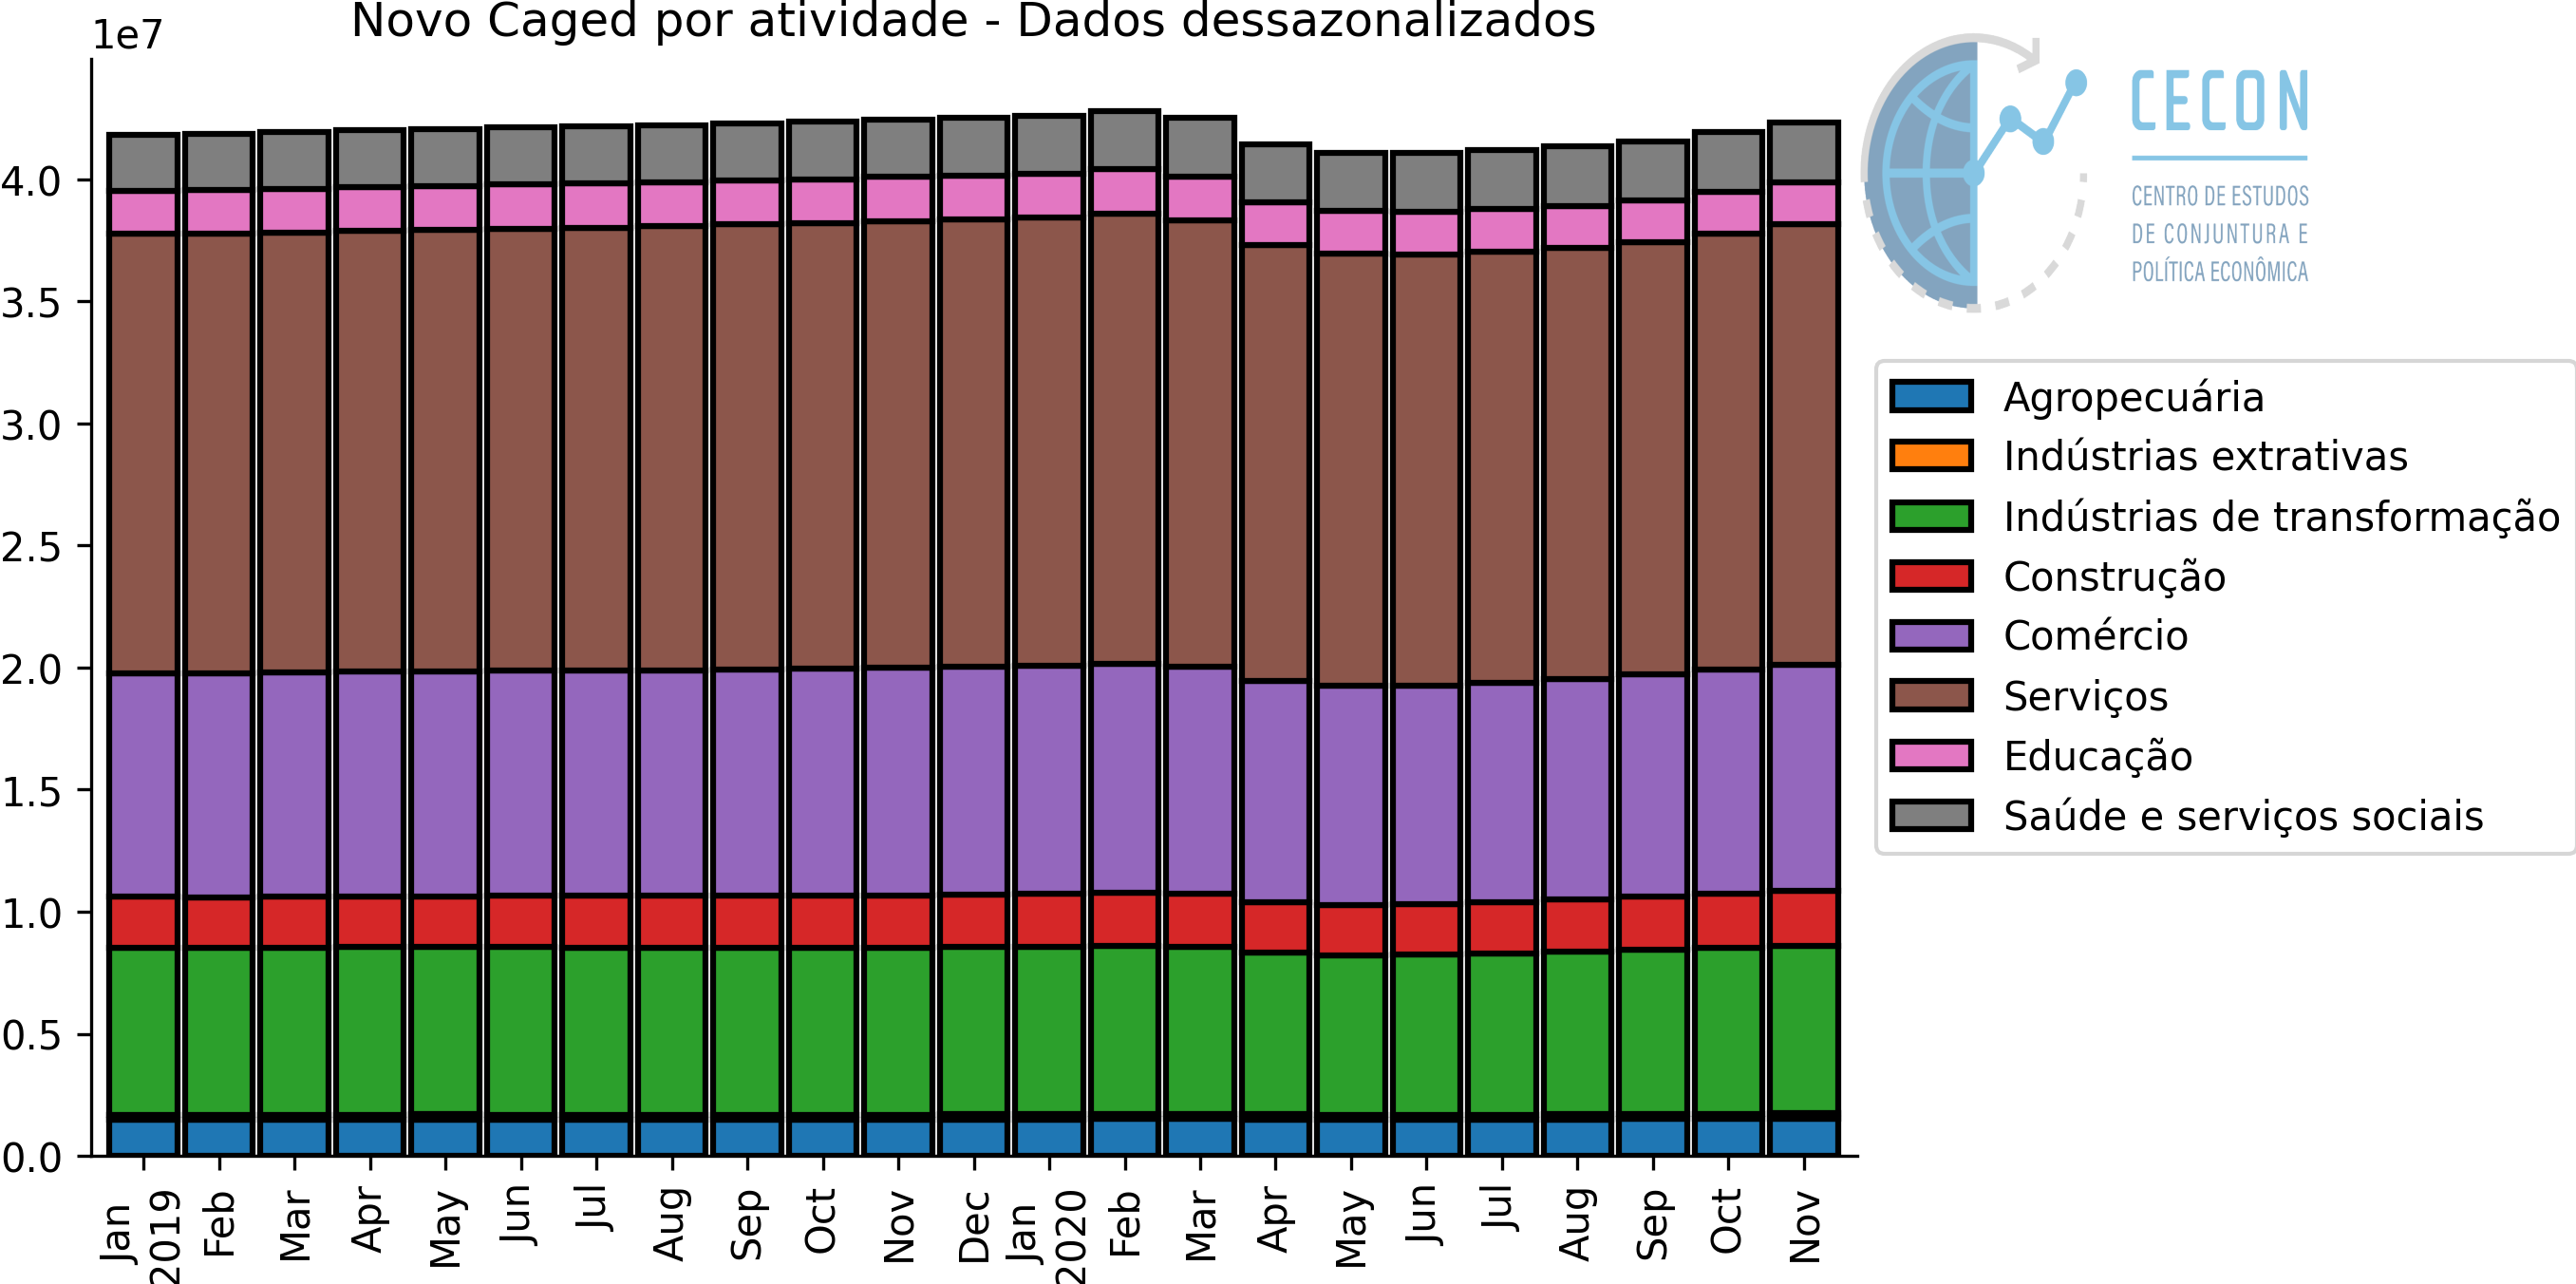
\includegraphics[width=.9\linewidth]{./figs/Emprego/NovoCaged_Atividade.png}
\end{center}



\subsection*{Taxa de desocupação}
\label{sec:orgcfafb82}

\begin{center}
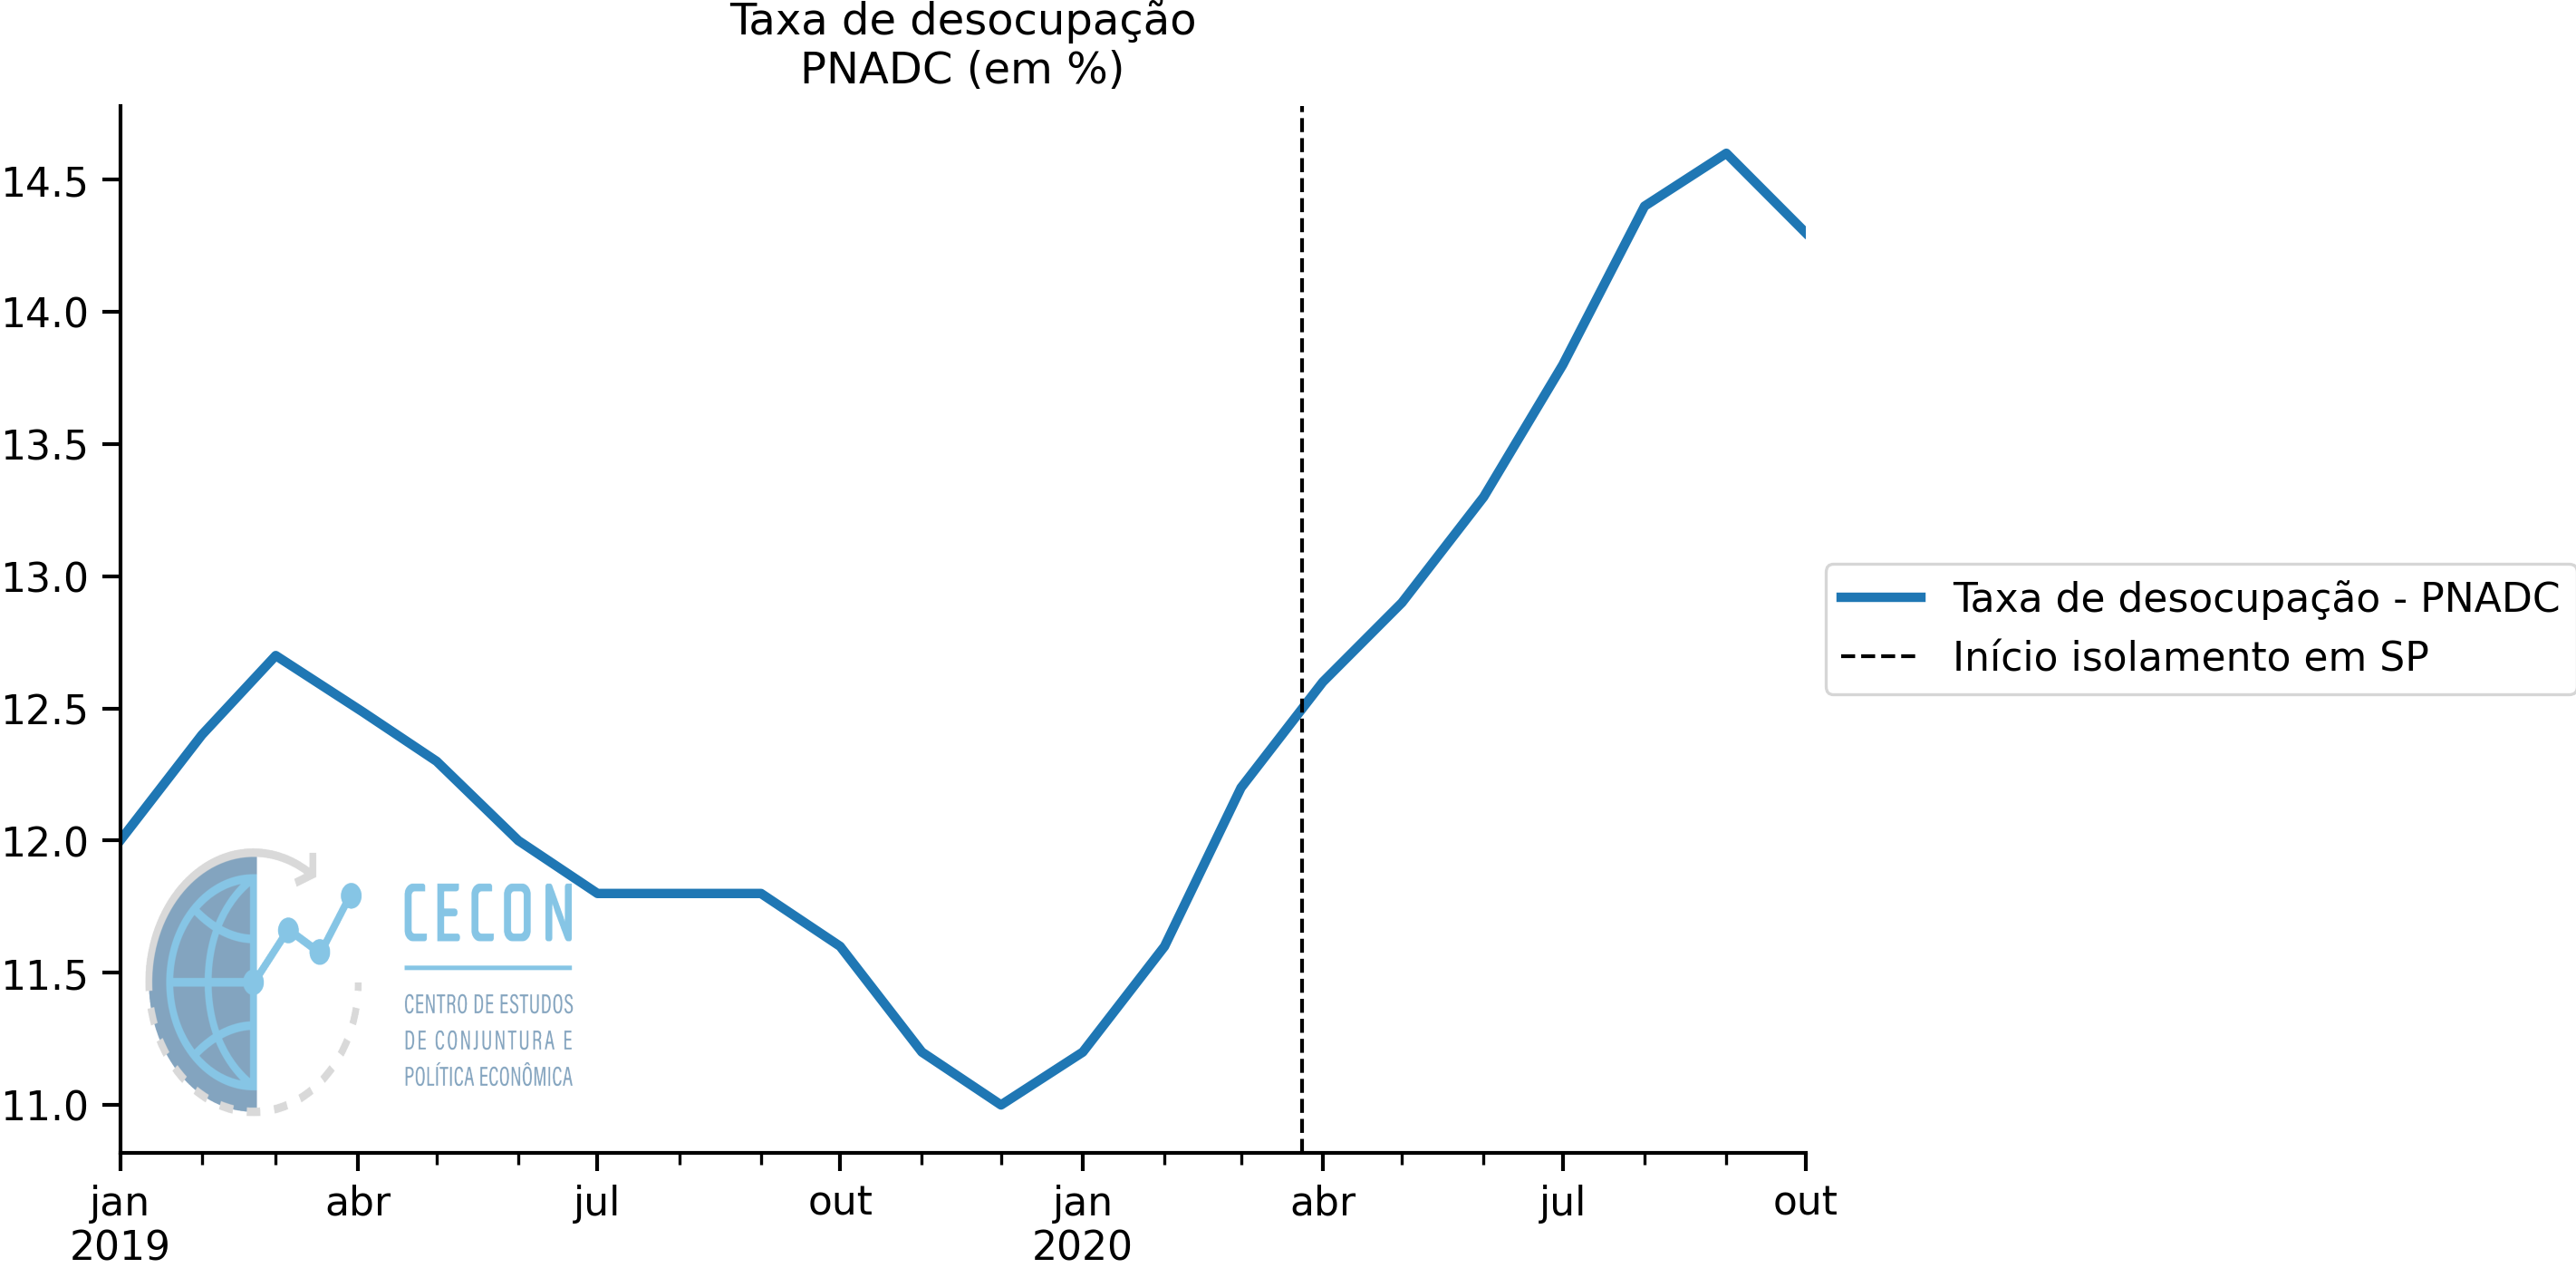
\includegraphics[width=.9\linewidth]{./figs/Emprego/TaxaDesocupacao.png}
\end{center}

\section*{PNAD-COVID}
\label{sec:orgb871e0a}
\subsection*{R trial}
\label{sec:org48fb016}
\subsection*{Home office - Por sexo e cor}
\label{sec:org95b8afa}




\begin{center}
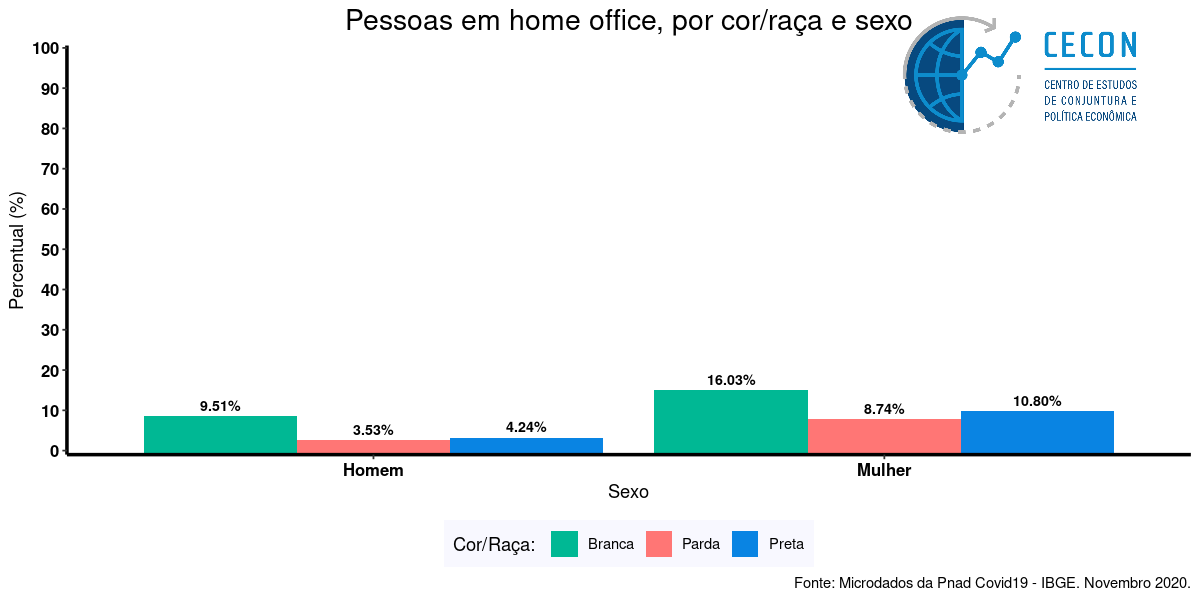
\includegraphics[width=.9\linewidth]{./figs/PNAD_COVID/home_sexo_cor.png}
\end{center}

\subsection*{Home office - Por Cor e Escolaridade}
\label{sec:org36076fd}
\begin{center}
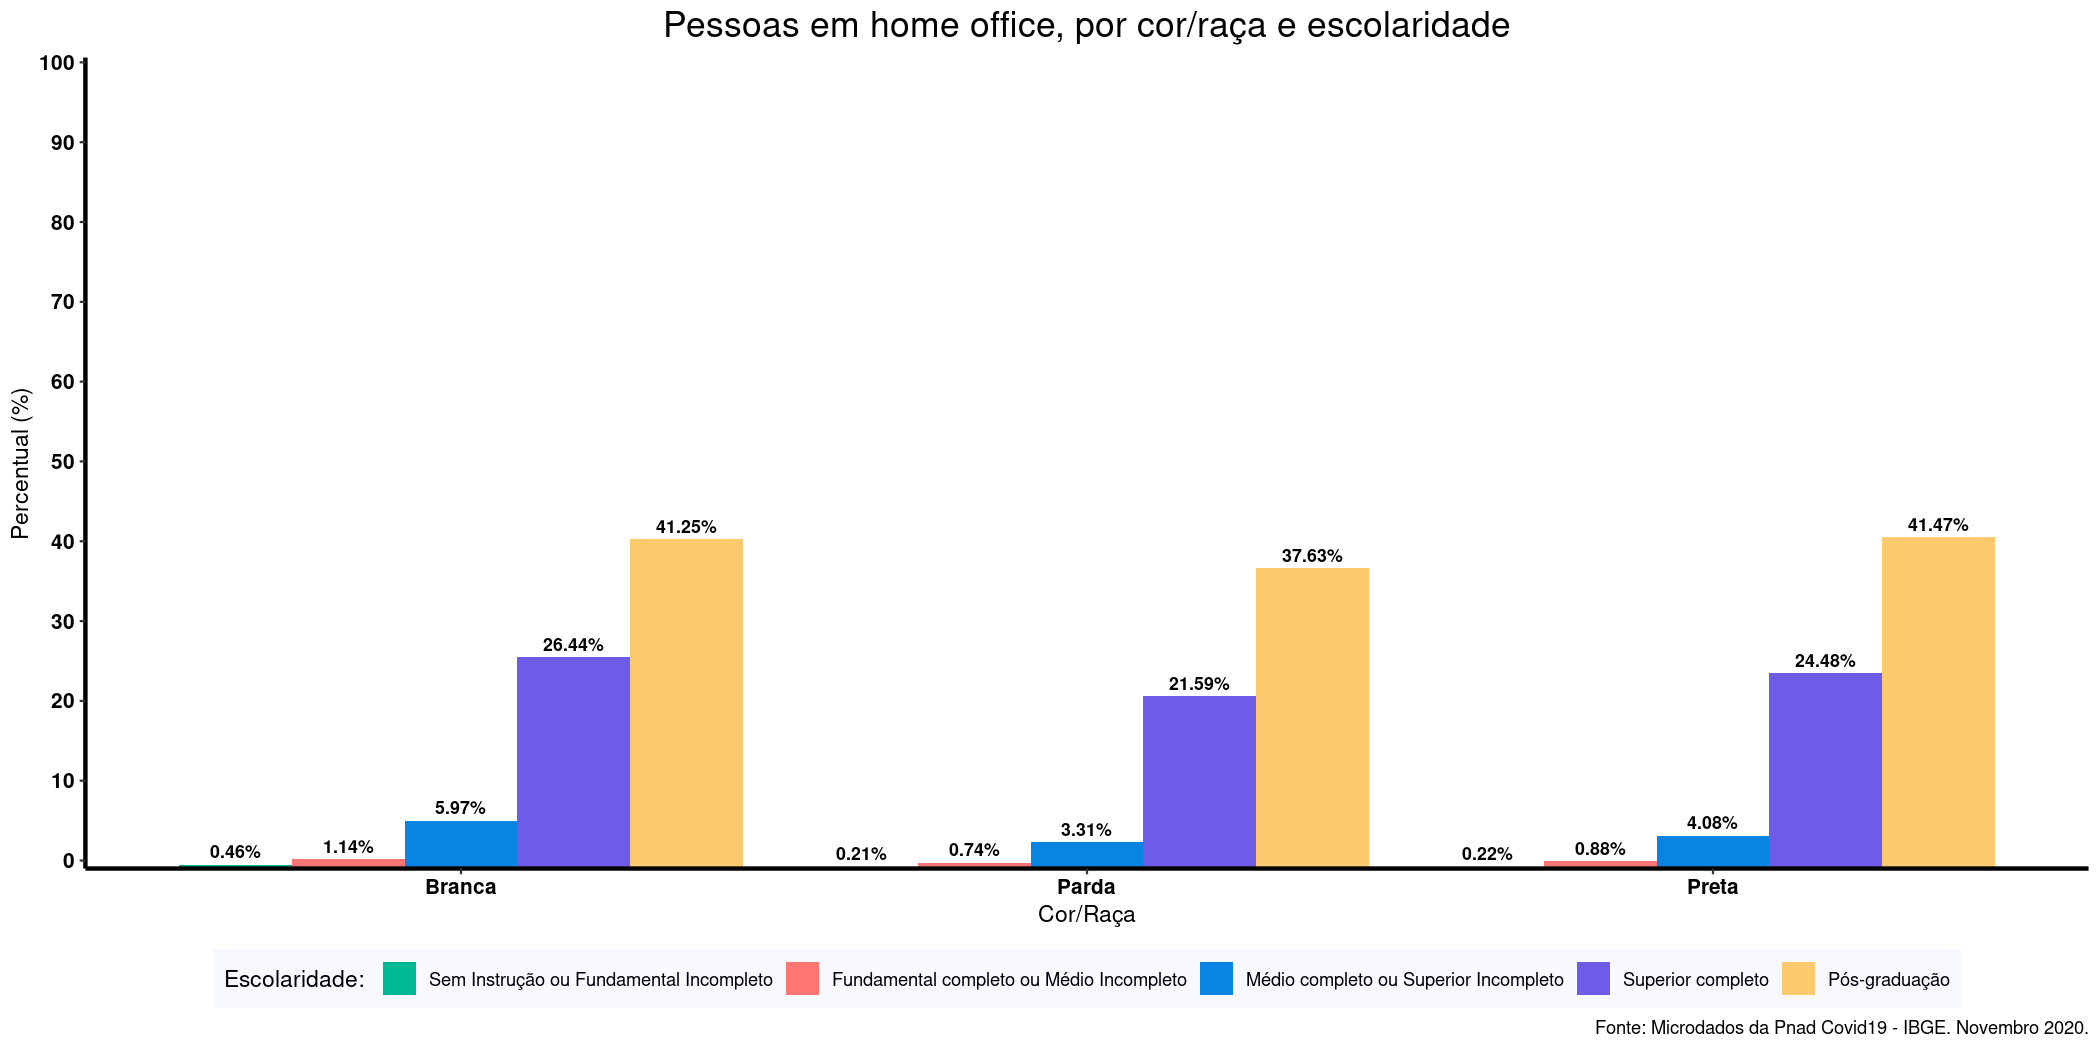
\includegraphics[width=.9\linewidth]{./figs/PNAD_COVID/home_edu_cor.png}
\end{center}
\subsection*{Home office - Por Cor e Idade}
\label{sec:org29da3a2}
\begin{center}
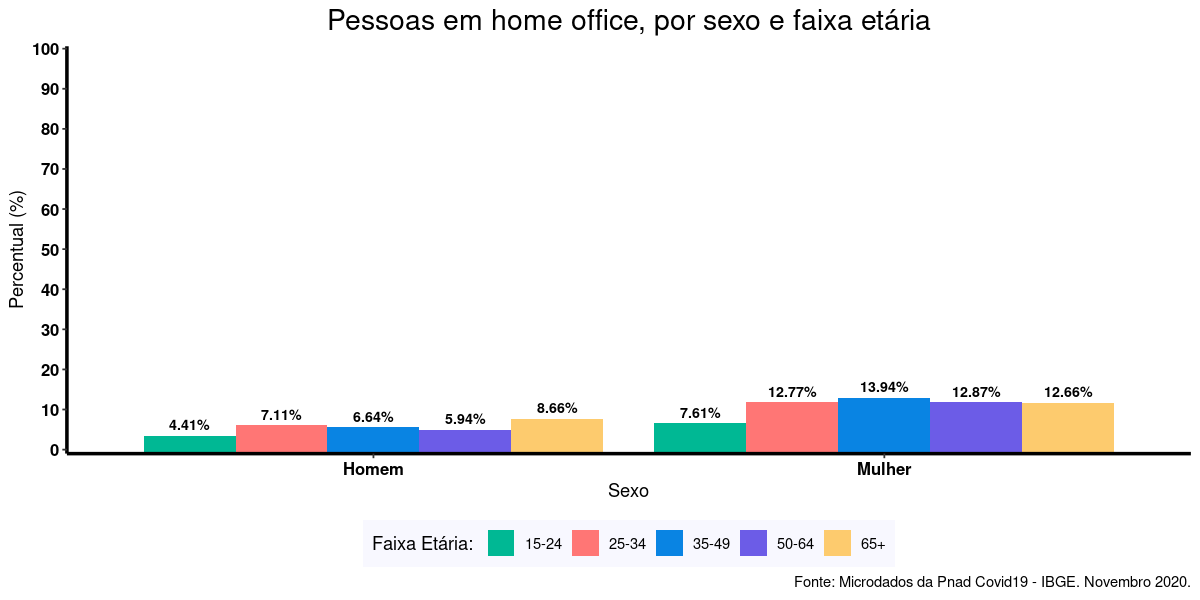
\includegraphics[width=.9\linewidth]{./figs/PNAD_COVID/home_sexo_idade.png}
\end{center}

\subsection*{Home office - Por Trabalho}
\label{sec:org8102984}
\begin{center}
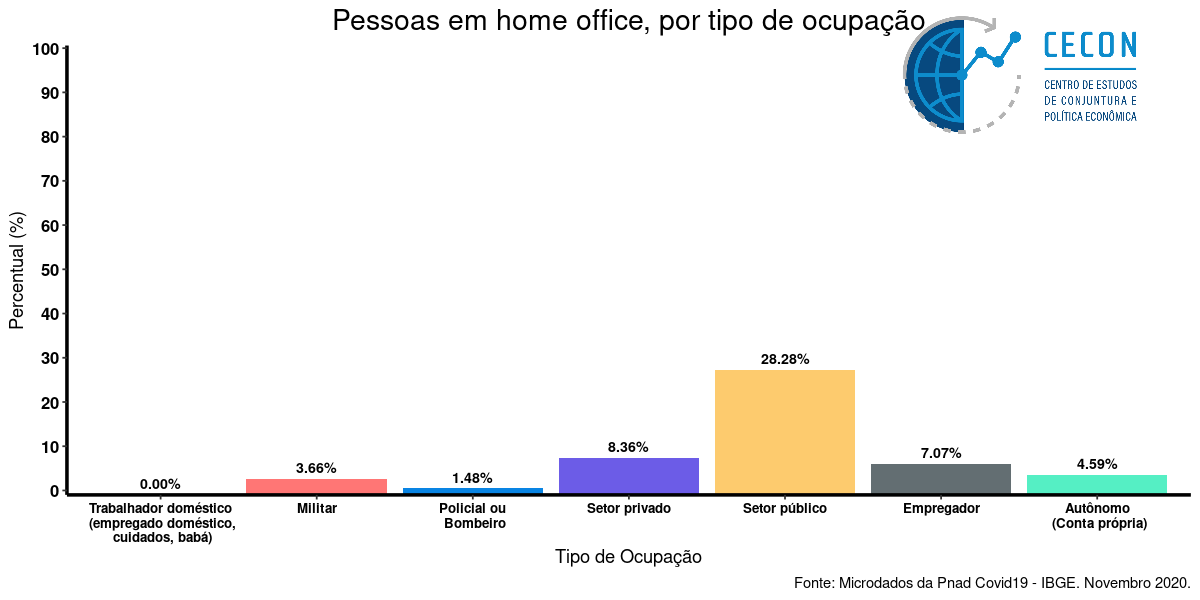
\includegraphics[width=.9\linewidth]{./figs/PNAD_COVID/home_emprego.png}
\end{center}

\subsection*{Home office - Por faixa salarial e cor}
\label{sec:org978debc}
\begin{center}
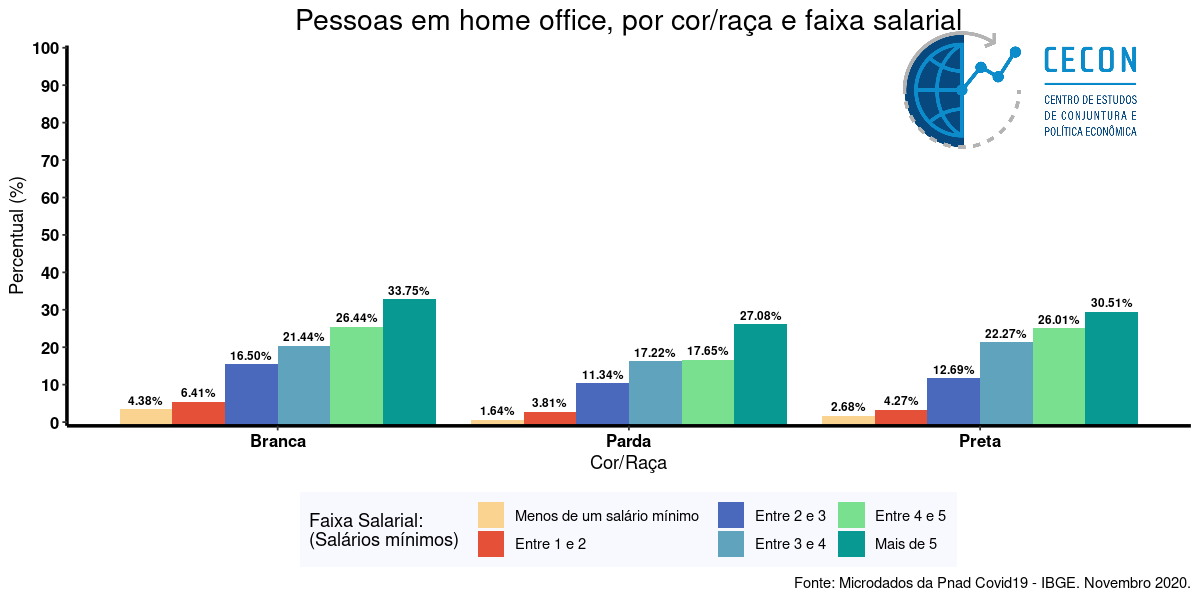
\includegraphics[width=.9\linewidth]{./figs/PNAD_COVID/home_renda.png}
\end{center}
\subsection*{Auxilio - Faixa Salarial}
\label{sec:org6fdc94c}
\begin{center}
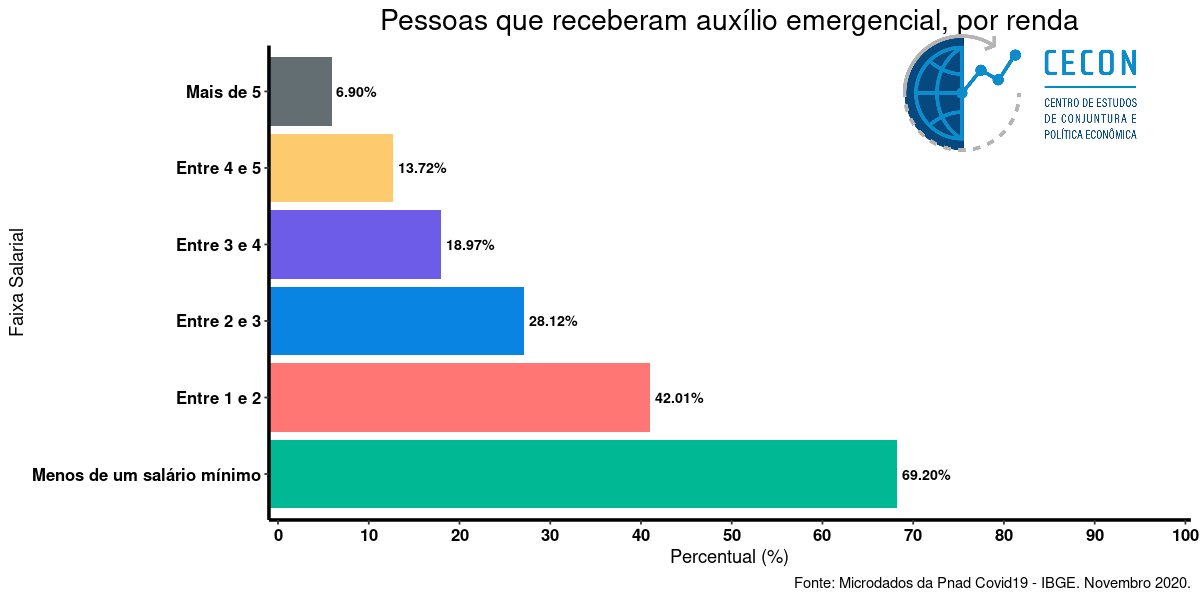
\includegraphics[width=.9\linewidth]{./figs/PNAD_COVID/auxilio_renda.png}
\end{center}
\subsection*{Auxilio - Por tipo do domicilio}
\label{sec:org7492cdd}
\begin{center}
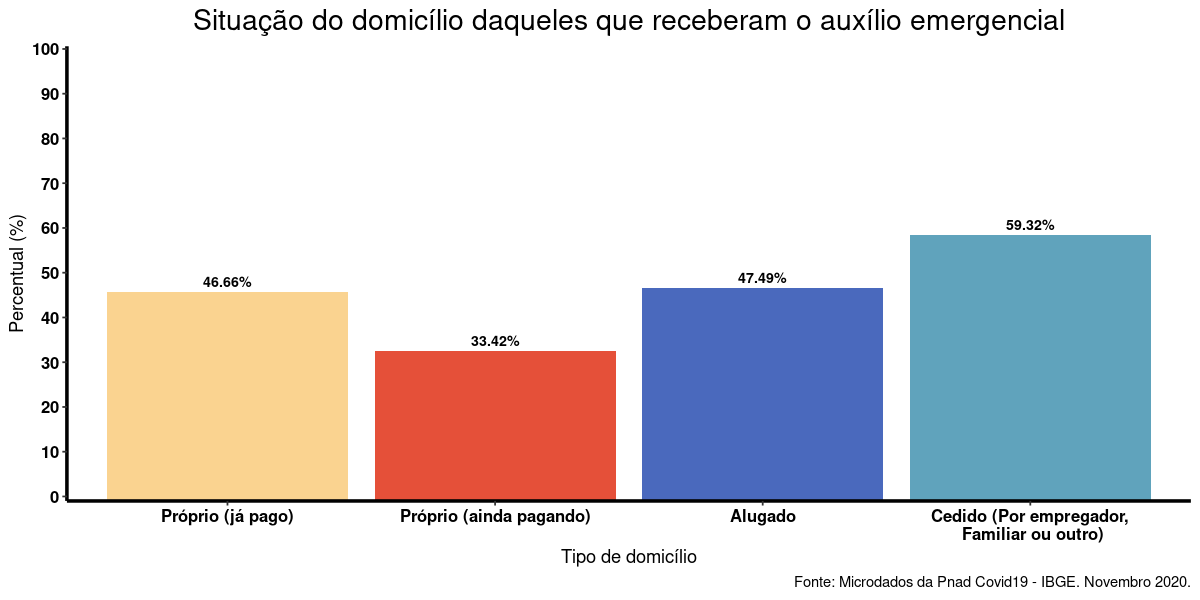
\includegraphics[width=.9\linewidth]{./figs/PNAD_COVID/auxilio_domicilio.png}
\end{center}
\subsection*{Auxilio - Sexo e Cor}
\label{sec:org5a78470}
\begin{center}
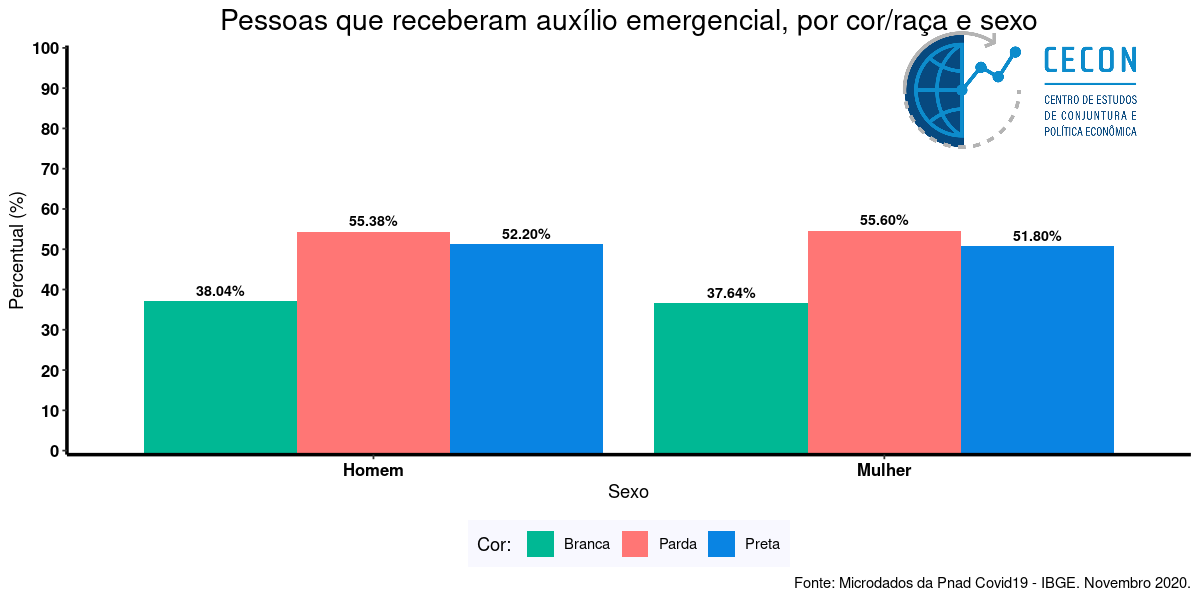
\includegraphics[width=.9\linewidth]{./figs/PNAD_COVID/auxilio_cor_sexo.png}
\end{center}


\section*{IMF Fiscal Monitor}
\label{sec:orgd729278}
\subsection*{Medidas fiscais em \% do PIB}
\label{sec:org1857c7c}

\begin{center}
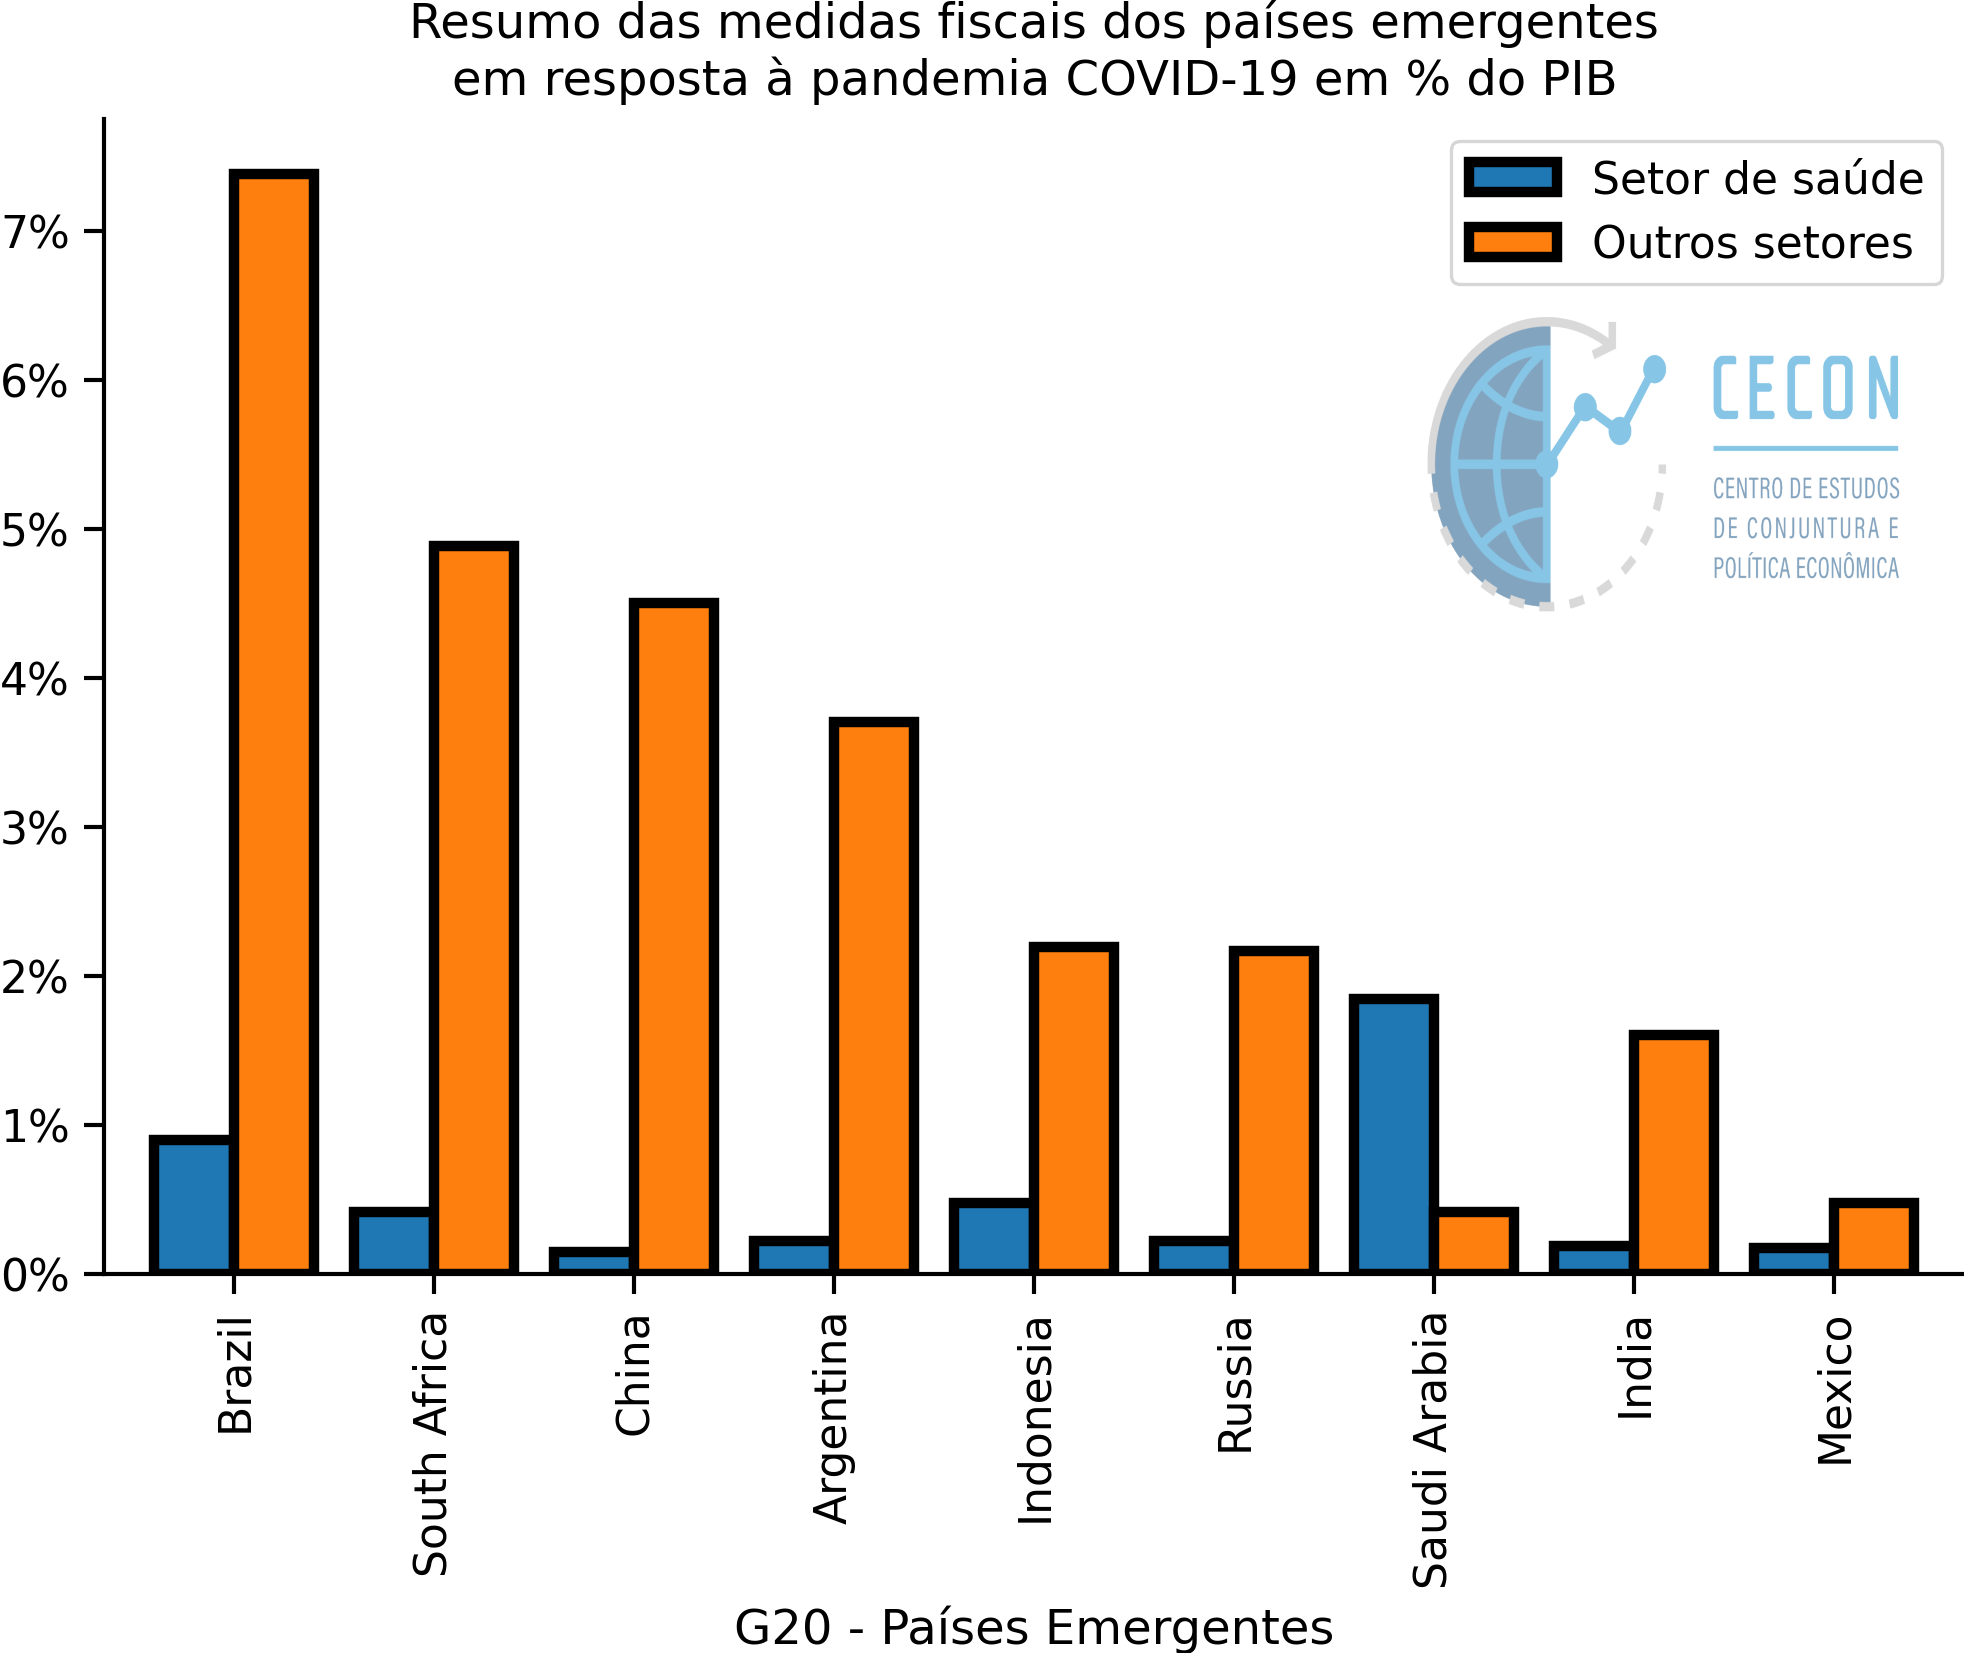
\includegraphics[width=.9\linewidth]{./figs/IMF/FiscalMonitor_Covid.png}
\end{center}

\subsection*{Medidas fiscais em \% do PIB: Setor de saúde/Outros setores}
\label{sec:org9526822}

\begin{center}
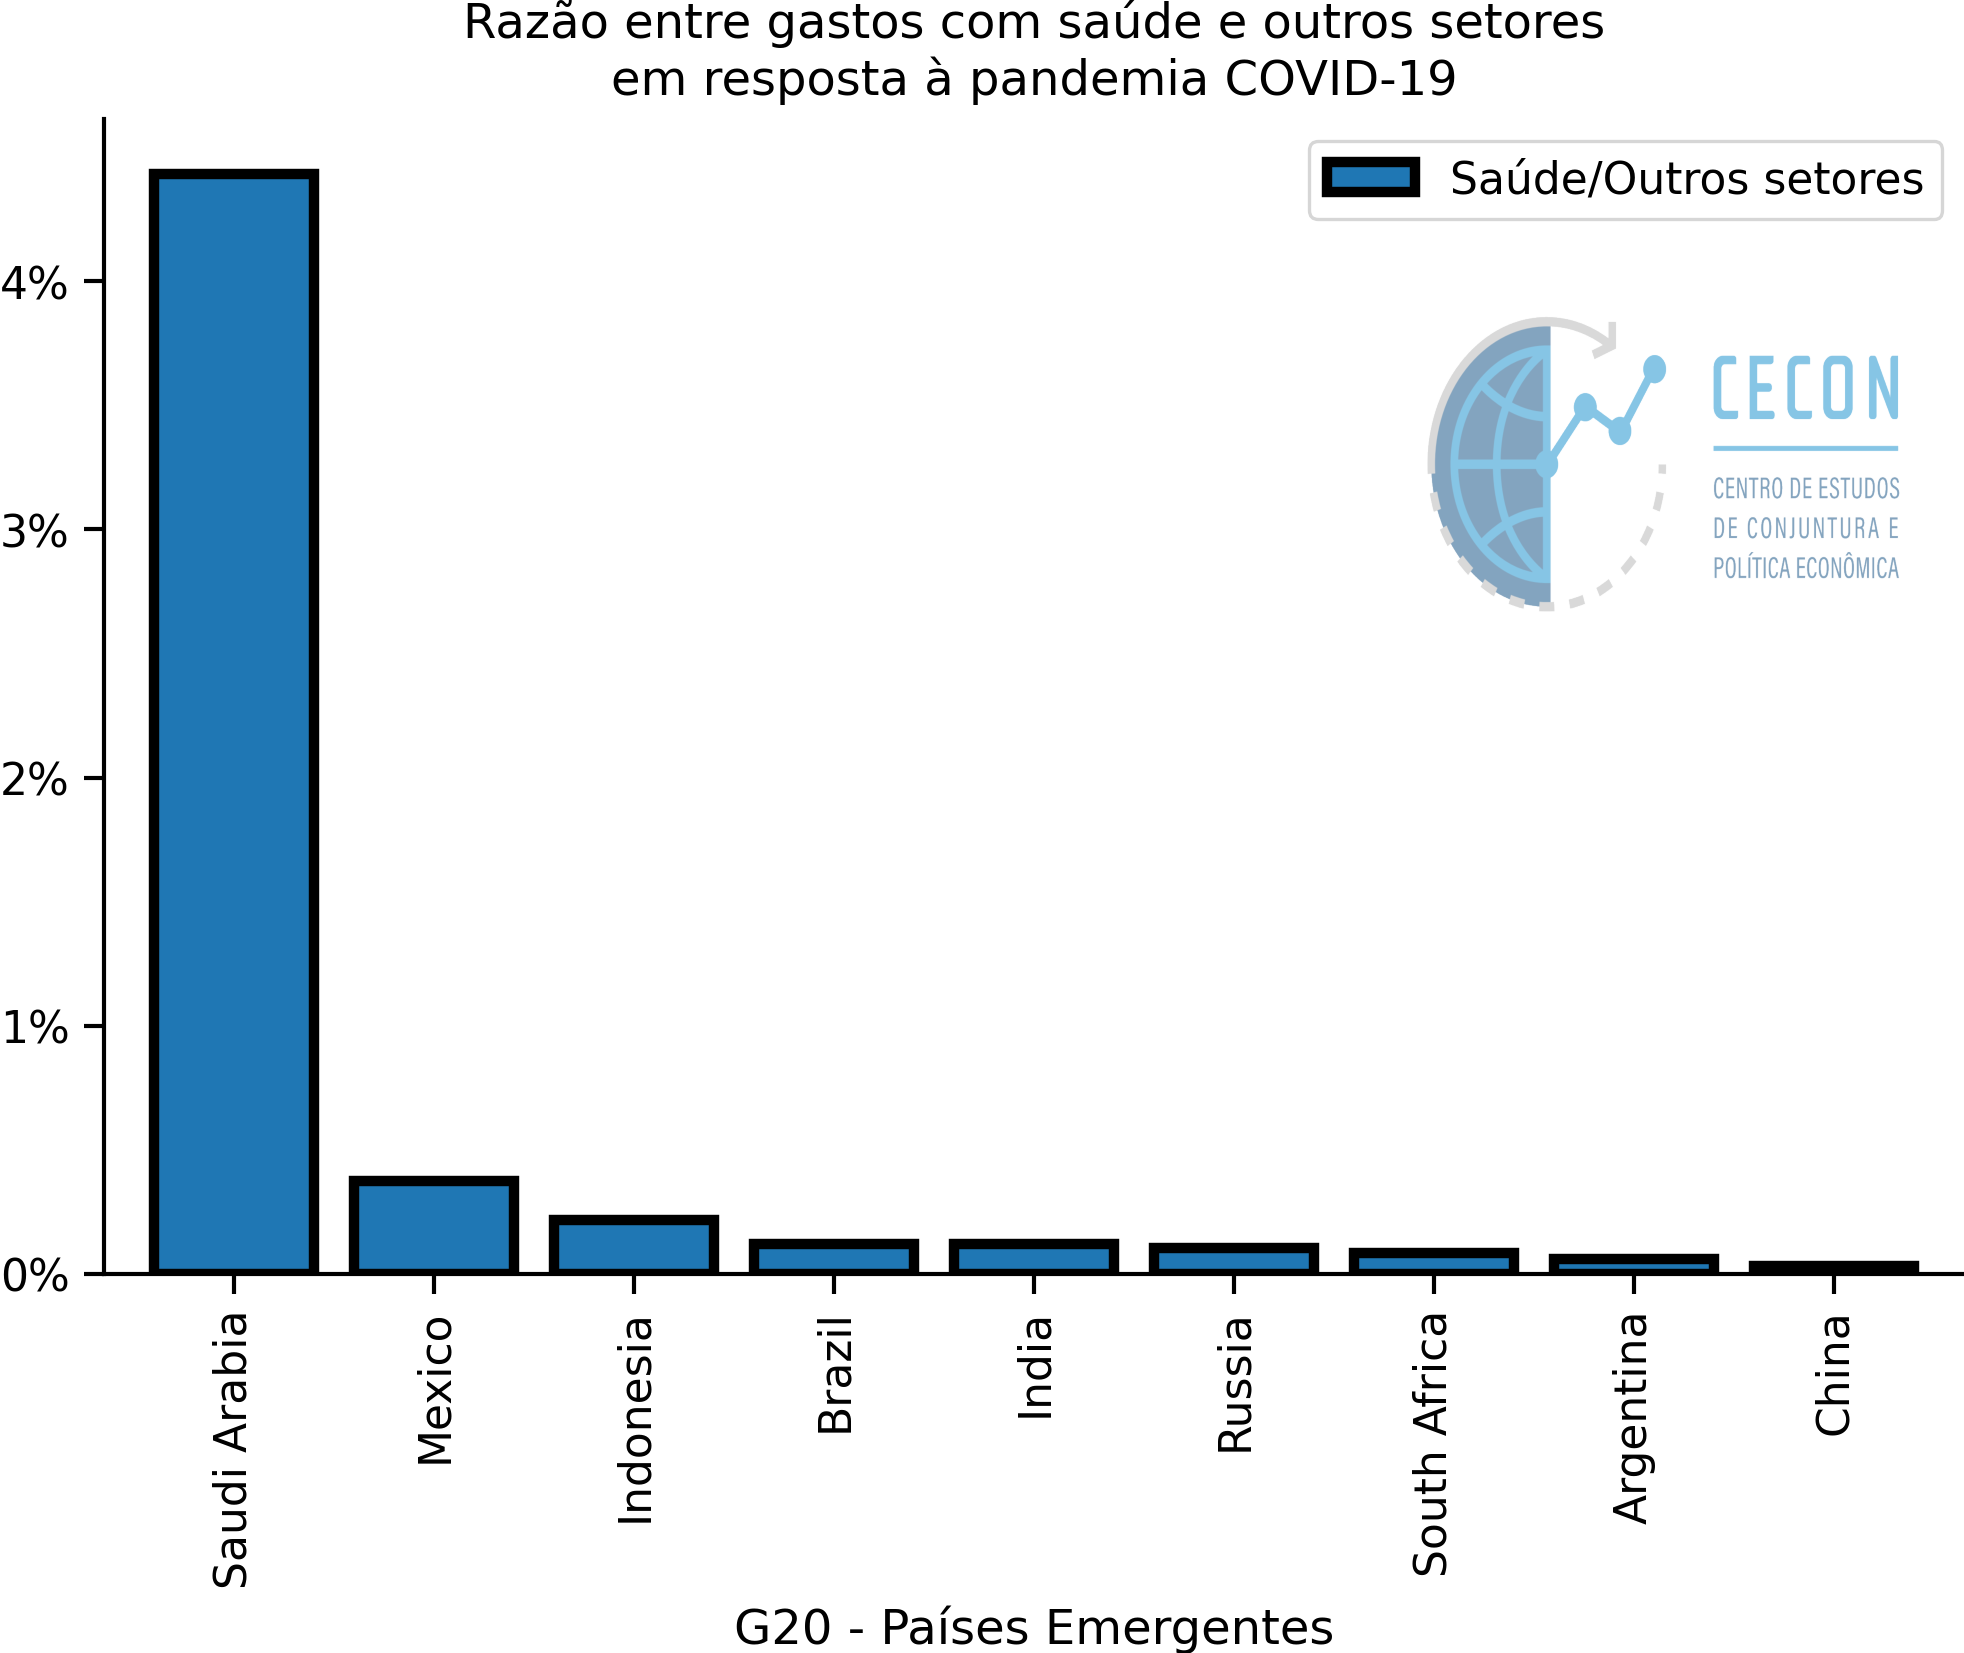
\includegraphics[width=.9\linewidth]{./figs/IMF/FiscalMonitor_Covid_ratio.png}
\end{center}

\subsection*{Medidas fiscais em \% do PIB: Setor de saúde/Total}
\label{sec:org9bc215c}

\begin{center}
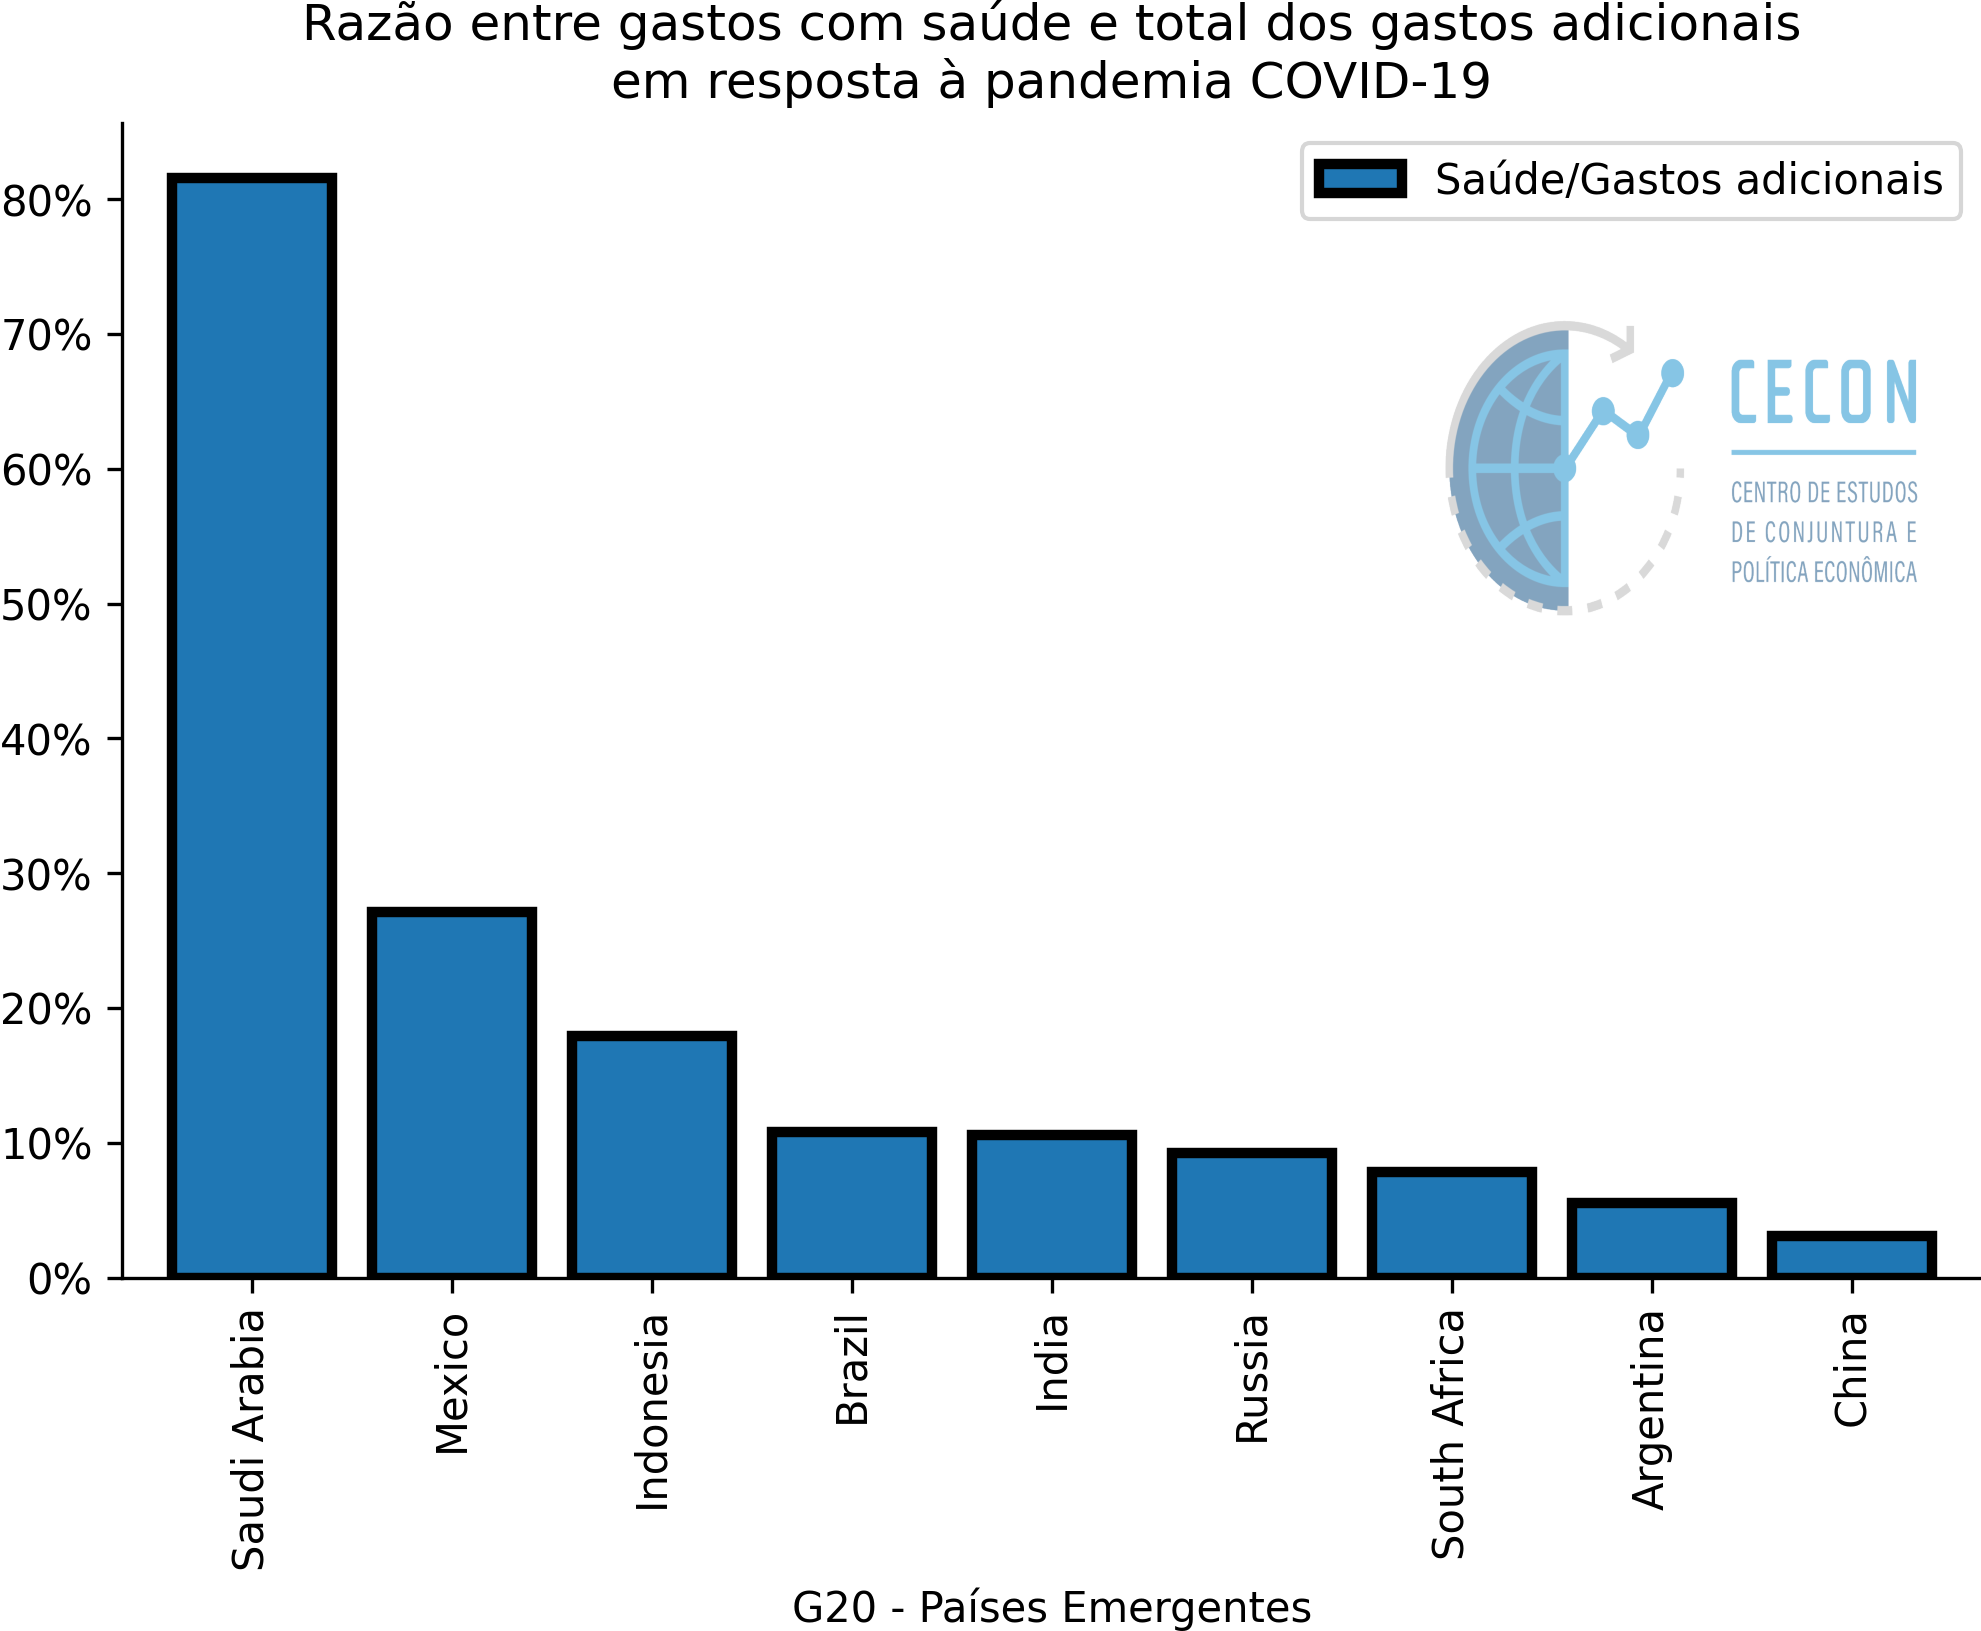
\includegraphics[width=.9\linewidth]{./figs/IMF/FiscalMonitor_Covid_total.png}
\end{center}
\end{document}